\documentclass[12pt]{article}
\usepackage[margin=1in]{geometry}
\usepackage[utf8]{inputenc}
\usepackage{multicol}
%\setlength{\columnsep}{1mm}
\usepackage{amsfonts}
\usepackage{booktabs}
\usepackage{siunitx}
\usepackage{float}
\usepackage[font={small}]{caption}
\usepackage[labelfont=bf]{caption}
\usepackage{lineno}
\usepackage{amsmath,amssymb,setspace,fancyhdr,geometry,url,color}
\usepackage{subfigure,graphicx,caption}
\usepackage{lscape,amsthm}
\usepackage{blindtext}
\usepackage{hhline}
\usepackage{arydshln}
\usepackage{verbatim}
\usepackage{dblfloatfix}
\usepackage{multirow}
\usepackage{graphicx}
\usepackage{xr}
\usepackage[document]{ragged2e}
%\usepackage[style=authoryear]{biblatex}
%\addbibresource{bib.bib}
%\usepackage{natbib}
%\bibliographystyle{authoryear}
\usepackage[backend=bibtex8,style=authoryear,natbib]{biblatex}
\addbibresource{bib.bib}

%\externaldocument{../PhaseIIPaper/main}
%\biboptions{authoryear, comma}
%%%%%%%%%%%%%%%%%%%%%%%%%%%%%%%%%%%%%%%%%%%%%%%%%%%%%%%%%%%%%%%%%%%%%%%%%
%%%%%%%%%%%%%%%%%%%%%%%%%%%%%%%%%%%%%%%%%%%%%%%%%%%%%%%%%%%%%%%%%%%%%%%%%%
\begin{document}

\centering{
\bf {\large Supplemental Material} \\
{\Large The GGCMI phase II emulators: global gridded crop model responses to changes in CO$_2$, temperature, water, and nitrogen (version 1.0)}
}\\

\vspace{3mm}

\centering{{\footnotesize James Franke$^{1, 2}$, 
Christoph M\"{u}ller$^3$, 
Joshua Elliott$^{2, 4}$, 
Alex C.\ Ruane$^5$, 
Jonas J\"{a}germeyr$^{3, 2, 4, 5}$,\\ 
Abigail Snyder$^6$, 
Marie Dury$^{7}$, 
Pete Falloon$^{8}$,
Christian Folberth$^9$, 
Louis Fran{\c{c}}ois$^{7}$, 
Tobias Hank$^{10}$, \\ 
R.\ Cesar Izaurralde$^{11, 12}$,
Ingrid Jacquemin$^7$, 
Curtis Jones$^{11}$, 
Michelle Li$^{2, 13}$, 
Wenfeng Liu$^{14, 15}$,\\
Stefan Olin$^{16}$, 
Meridel Phillips$^{5, 17}$, 
Thomas A.\ M.\ Pugh$^{18, 19}$, 
Ashwan Reddy$^{11}$, 
Karina Williams$^{8,20}$, \\
Ziwei Wang$^{1, 2}$, 
Florian Zabel$^{10}$, 
and Elisabeth Moyer$^{1, 2}$
~\\}}
\medskip

\centering{
{\scriptsize 
1. Department of the Geophysical Sciences, University of Chicago, Chicago, IL, USA. \\
2. Center for Robust Decision-making on Climate and Energy Policy (RDCEP), University of Chicago, Chicago, IL, USA. \\
3. Potsdam Institute for Climate Impact Research, Member of the Leibniz Association, Potsdam, Germany. \\
4. Department of Computer Science, University of Chicago. \\
5. NASA Goddard Institute for Space Studies, New York, NY, United States. \\
6. Joint Global Change Research Institute, Pacific Northwest National Laboratory, College Park, MD, USA. \\
7. Unit{\'{e}} de Mod{\'{e}}lisation du Climat et des Cycles Biog\'eochimiques, UR SPHERES, Institut d'Astrophysique et de G\'eophysique, University of Li\`ege, Belgium. \\
8. Met Office Hadley Centre, Exeter, United Kingdom. \\
9. Ecosystem Services and Management Program, IIASA, Laxenburg, Austria. \\
10. Department of Geography, Ludwig-Maximilians-Universit\"{a}t, Munich, Germany. \\
11. Department of Geographical Sciences, University of Maryland, College Park, MD, USA. \\
12. Texas Agrilife Research and Extension, Texas A\&M University, Temple, TX, USA.  \\
13. Department of Statistics, University of Chicago, Chicago, IL, USA. \\
14. EAWAG, Swiss Federal Institute of Aquatic Science and Technology, D\"{u}bendorf, Switzerland. \\
15. Laboratoire des Sciences du Climat et de l'Environnement, LSCE/IPSL, CEA-CNRS-UVSQ, Universit\'{e} Paris-Saclay, F-91191 Gif-sur-Yvette, France. \\
16. Department of Physical Geography and Ecosystem Science, Lund University, Lund, Sweden. \\
17. Earth Institute Center for Climate Systems Research, Columbia University, New York, NY, USA.  \\
18. School of Geography, Earth and Environmental Sciences, University of Birmingham, Birmingham, UK.  \\
19. Birmingham Institute of Forest Research, University of Birmingham, Birmingham, UK. \\
20. Global Systems Institute, University of Exeter, Laver Building, North Park Road, Exeter, EX4 4QE, UK. \\
}}

{\scriptsize \tableofcontents}

%%%%%%%%%%%%%%%%%%%%%%%%%%%%%%%%%%%
\clearpage
%%%%%%%%%%%%%%%%%%%%%%%%%%%%%%%%%%%

\renewcommand{\thefigure}{S\arabic{figure}}
\renewcommand{\thetable}{S\arabic{table}}

\section{Sampling in variable space and cultivated area}
\begin{justify}
	Simulation sampling across the defined variable space is not uniform in the GGCMI Phase II experiment, with only some models providing all cases in the protocol. 
  Figure \ref{fig:numbersims} compares the sampling density of the models used in the emulator analysis. 
\end{justify}

\begin{figure}[h!]
  \centering
  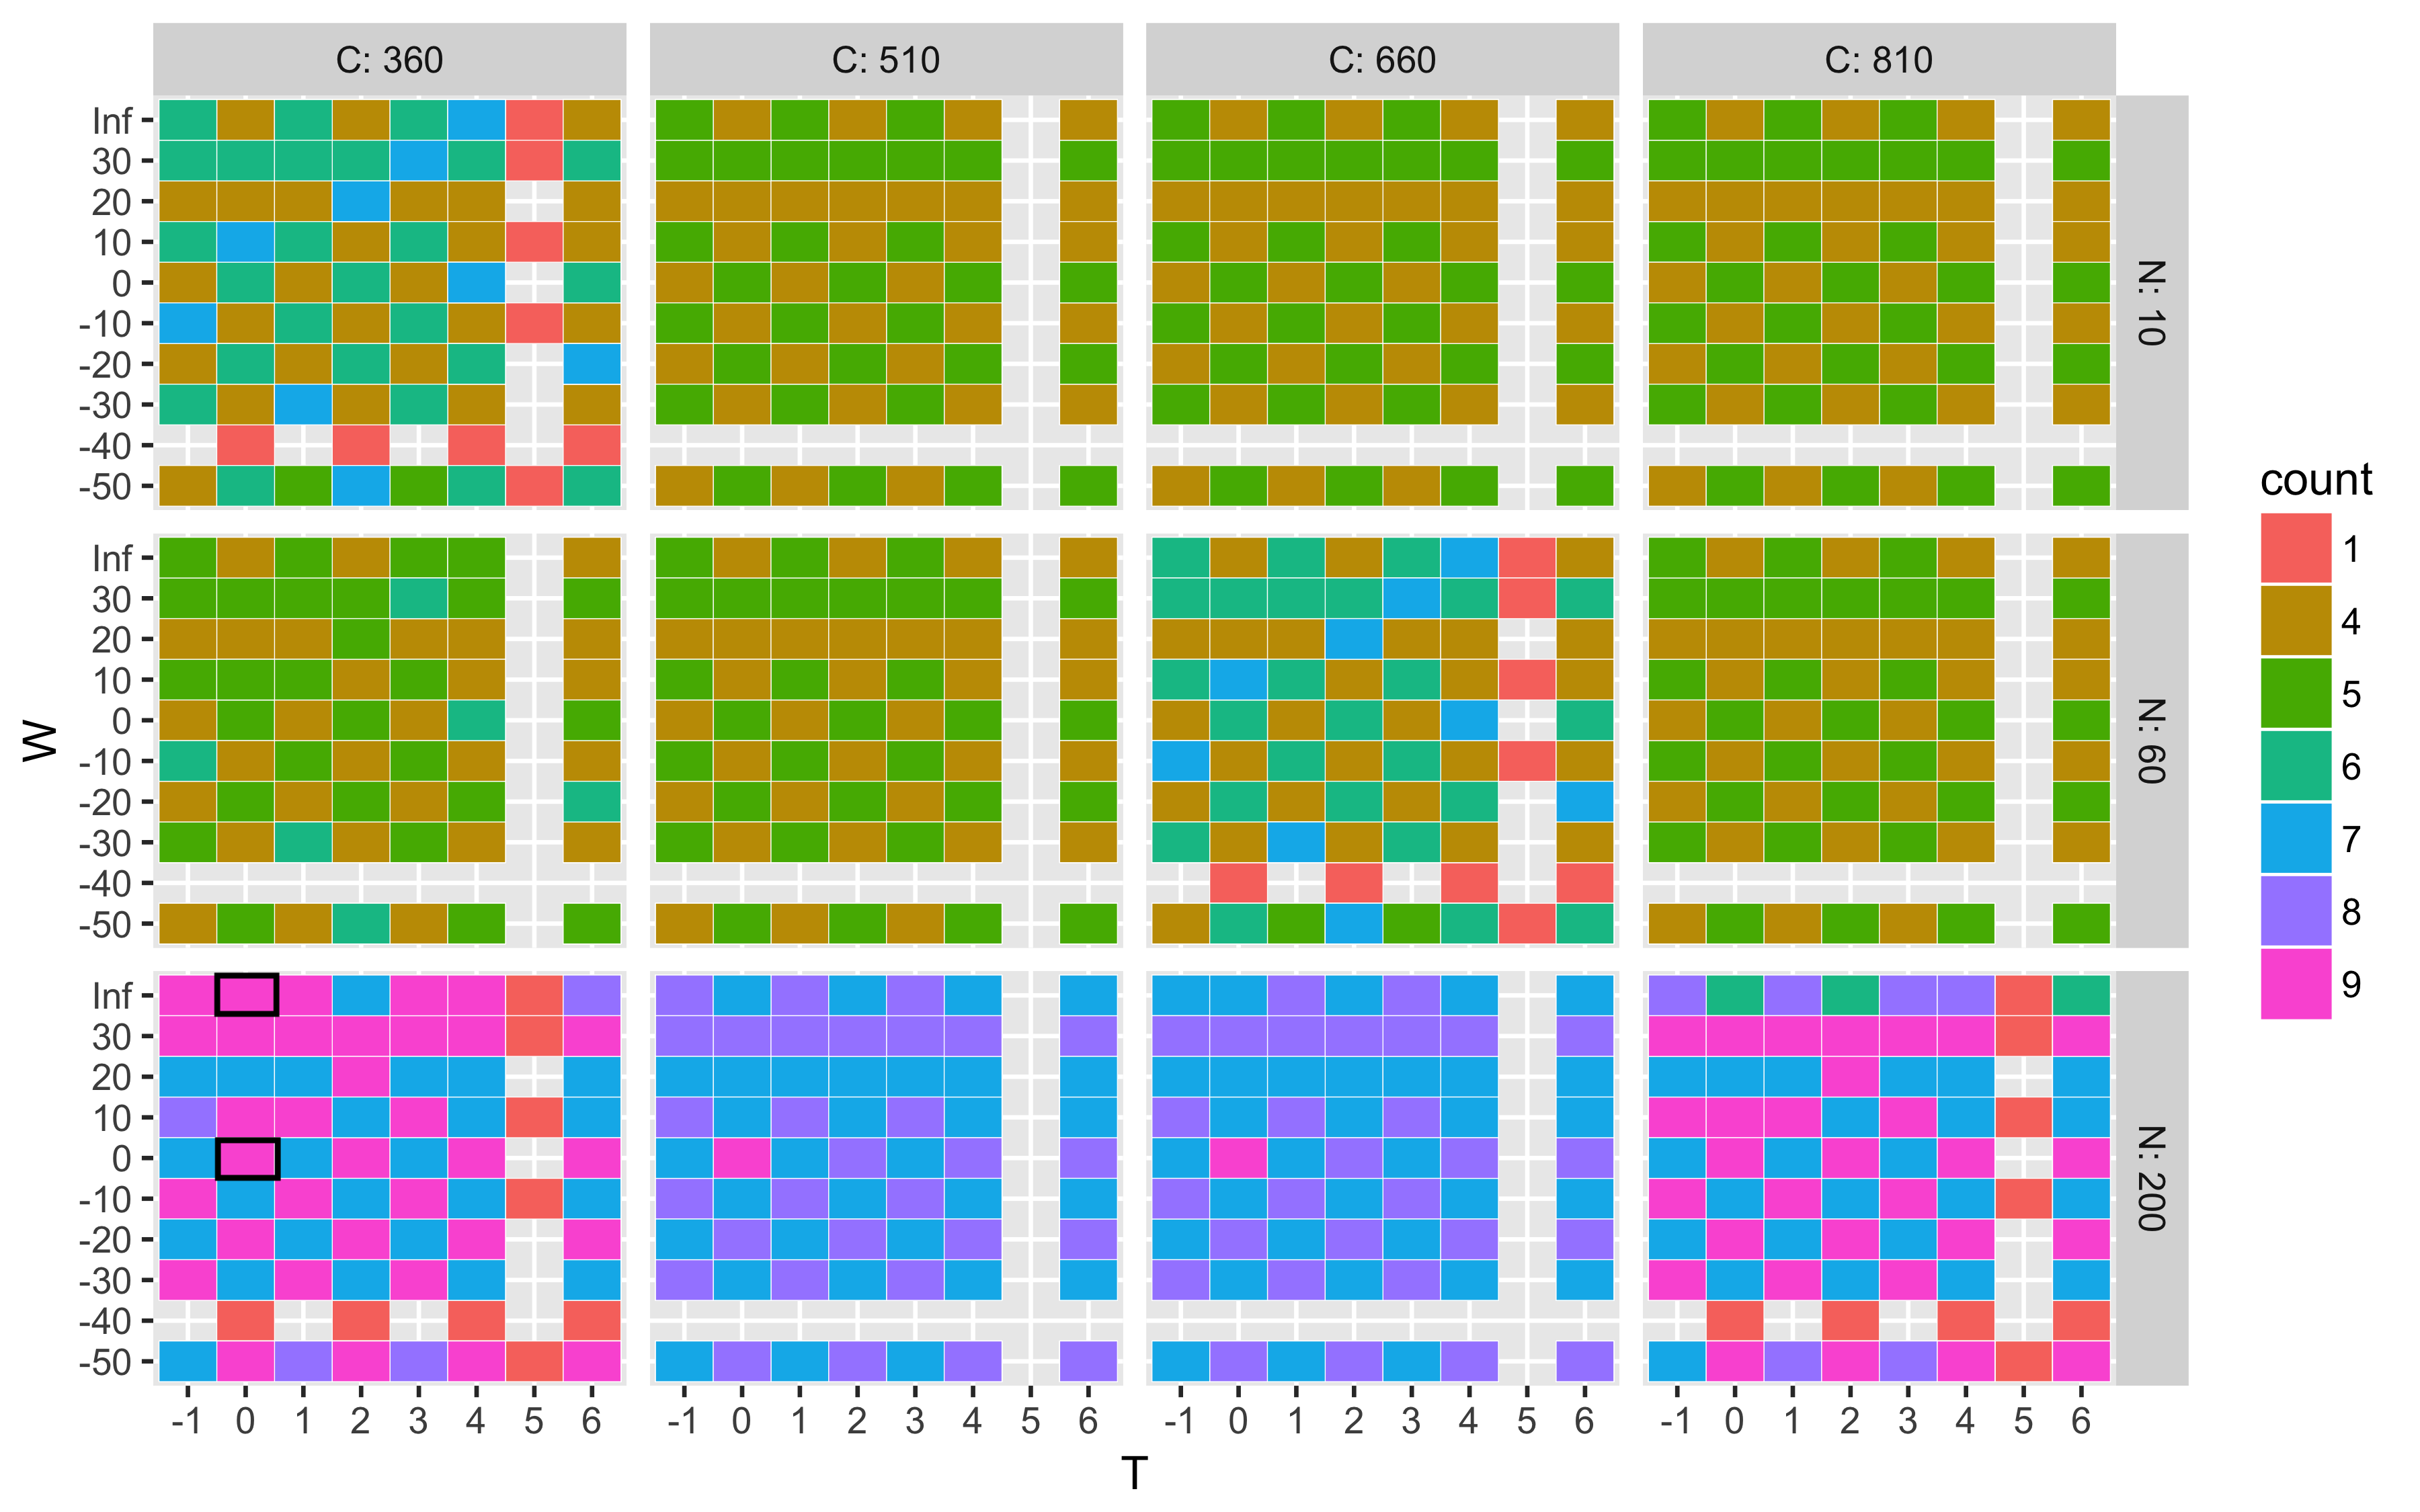
\includegraphics[width=\textwidth]{s_how_many_simulations.png}
  \caption{
  Heatmap illustrating the number of models providing simulations for each of the scenarios in CTWN variable space. Black boxes mark the ``baseline'' cases for rainfed and irrigated simulations.
	The maximum number is 9, the number of models included in the emulator analysis. (That is, we exclude here the three GGCMI Phase II models not included in the emulator analysis.)  For cases with N levels lower than 200 kg/ha, the maximum number of models is 6 since three models (CARAIB, JULES, and PROMET) do not represent varying N levels. One model (GEPIC) provided additional simulations at T+5 not specified by the protocol; these are not used in emulation.
  	Normalized error calculations are run only over scenarios in which 9 models contribute simulations (pink boxes).  }
  \label{fig:numbersims}
\end{figure}

\clearpage
\begin{figure}[h!]
    \centering
    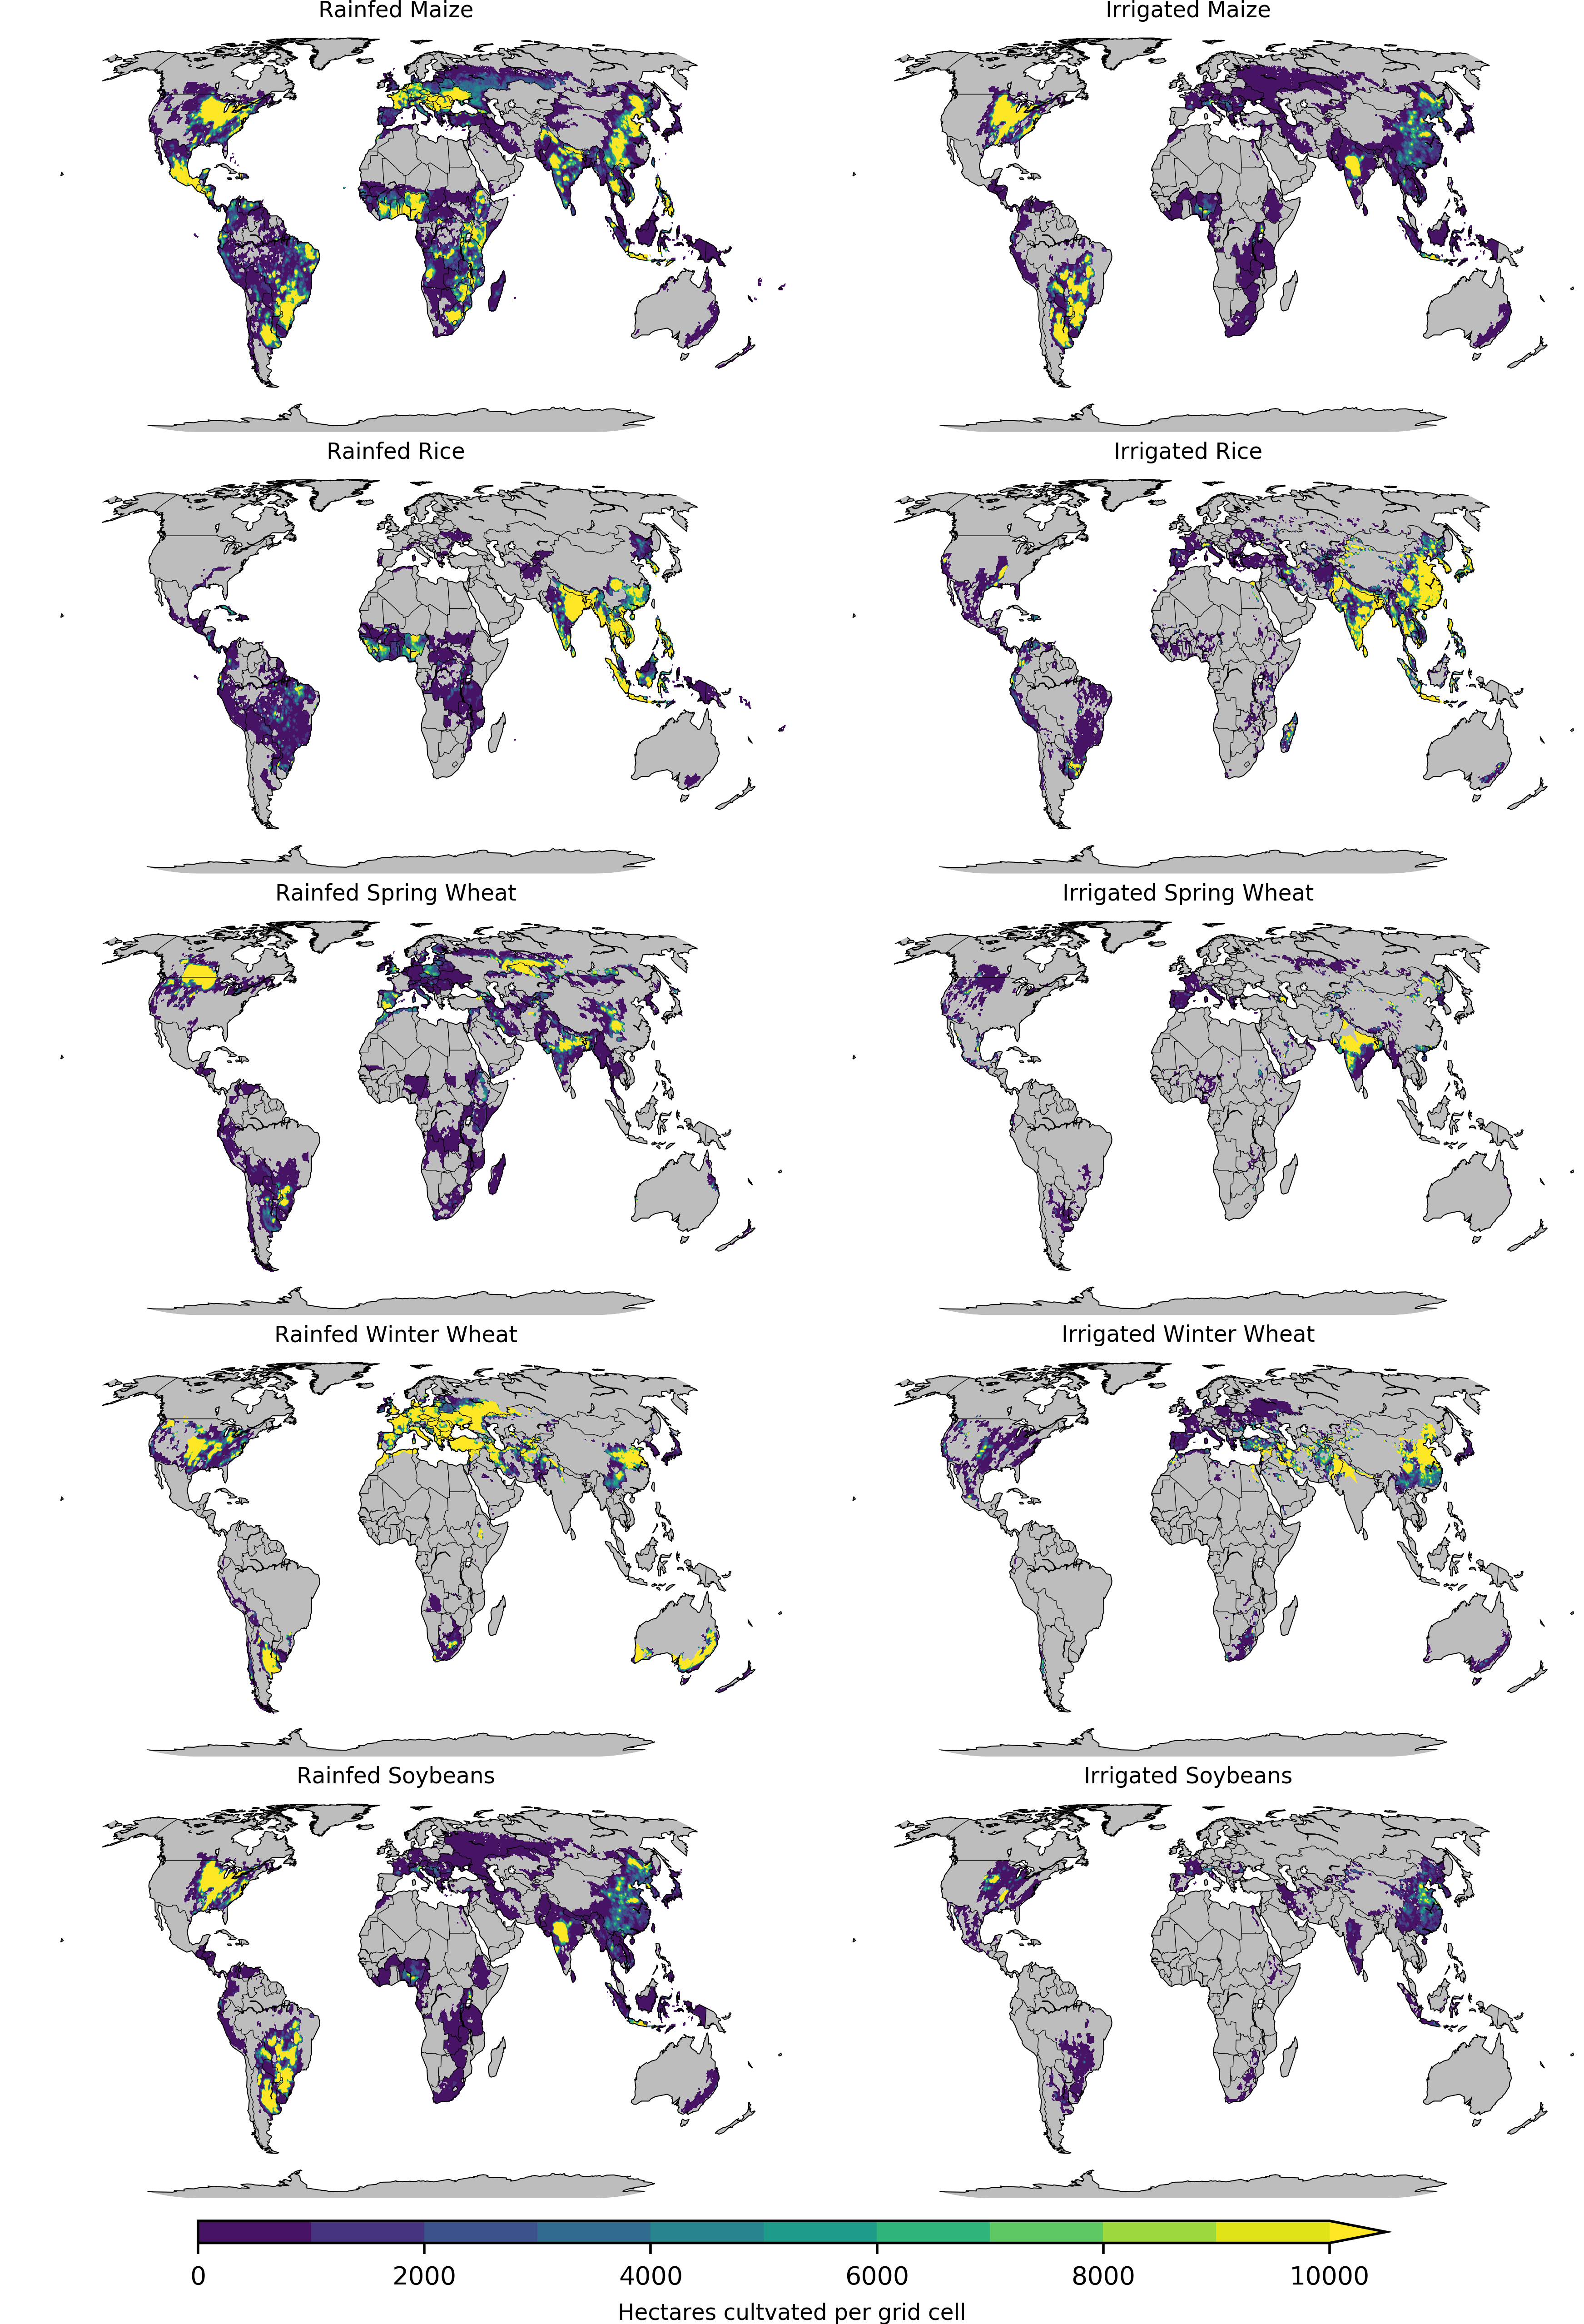
\includegraphics[width=14cm]{cult_area.png}\\
    \caption{
    Presently cultivated area in the real world for rainfed (left) and irrigated (right) crops, from the MIRCA2000 dataset \parencite{Portmann2010}. 
    %Blue areas show grid-cells with more that 20,00 hectares of crop cultivated, and gray areas those with more that 10 hectares cultivated. 
    Data are taken directly from the MIRCA2000 dataset  for maize, rice, and soy. 
    Winter and spring wheat areas are adapted from MIRCA2000 and sorted by growing season.
    }
    \label{fig:irrarea}
\end{figure}

\clearpage
\section{Variability changes in future climate projections}
\begin{justify}
Because the GGCMI Phase II simulation dataset does not sample across changes in climate variability, large impacts to yields driven by future changing variability would decrease the practical utility of the emulator for impacts assessments.
	We therefore assess the scale of potential future changes in temperature variability, in RCP8.5 simulations from the five climate models used in ISIMP \parencite[the Inter-Sectoral Impact Model Intercomparison Project;][]{Warszawski3228, Frieler2017}.
 In manuscript section 4.3 we use one of these climate simulations, that from HadGEM2-ES, to assess the ability of GGCMI emulators to reproduce yield changes simulated under more realistic climate projections. We choose the HadGEM2-ES model because it shows the largest variability changes, and therefore provides a stricter test of the utility of a GGCMI emulator.
 Table S1 summarizes daily T$_{max}$ variability changes for each crop and model weighted by production. 
	Figures S3 and S4 below show changes in variability in minimum and maximum temperatures in the HadGEM2 simulation for each crop growing season and area, and Figure S5 shows changes in daily T$_{max}$ variability for maize across the 4 additional ISIMIP climate simulations. (Compare to Figure S3 upper left panel.)
	Most crop models included in GGCMI phase II take daily minimum and maximum temperature as inputs, though PROMET and JULES take sub-daily temperature inputs.
	  
%Changes in variability are typically larger for maximum temperature than for minimum temperature in the climate models included here (some models show decreases in variability in minimum daily temperatures).

\end{justify}

\begin{table}[ht]
{\small
    \caption{
	    Global production-weighted fractional change in growing season daily maximum temperature variability under RCP8.5 for the five climate models included in the ISIMIP project (a subset of the CMIP-5 archive). 
    Value for each crop and model is mean within-growing season temperature standard deviation across 30 growing seasons of 2070-2099 relative to that for 1981-2010, with grid-cell values weighted by 
	   LPJmL model simulated yields and current cultivation area (MIRCA).
    Values in parenthesis are the change in variability by the same metric for daily minimum temperature within the growing season.
    The HadGEM2-ES model is highlighted in bold because this model is used for our emulator evaluation in manuscript Section 4.3. The HadGEM2-ES model is chosen because it shows the highest changes in variability.
    }
    \begin{tabular}{l | c | c | c | c | c} 
        \hline
        \textbf{Model}        & \textbf{Maize \%} & \textbf{Soybean \%} & \textbf{Rice \%} & \textbf{S. Wheat \%} & \textbf{W. Wheat \%} \\ \hline
        \textbf{HadGEM2-ES}   & \textbf{9.7 (2.1)}  & \textbf{10.4 (-0.6)}  & \textbf{10.1 (-3.3)}  & \textbf{6.4 (4.7)}  & \textbf{3.6 (1.7)}  \\ \hline
        \textbf{GFDL-ESM2M}   & 3.6 (0.9)  & 3.4 (0.6)  & 2.7 (-0.3)  & 1.2 (-0.3) & 2.0 (1.0)  \\ \hline
        \textbf{NorESM1-M}    & 6.7 (-1.1)  & 6.5 (-4.0)  & 5.9 (-3.5)  & 4.5 (3.3)  & 2.4 (0.8)    \\ \hline
        \textbf{IPSL-CM5A-LR} & 3.3 (3.3)  & 3.4 (0.6)  & 3.4 (1.4)  & 1.4 (2.3)  & 1.2 (1.3)  \\ \hline
        \textbf{MIROC-ESM}    & 4.0 (1.2)  & 3.1 (0.1)  & 0.4 (-5.1)  & 2.2 (-0.3)  & 2.6 (2.3)  \\ \hline
    \end{tabular}
}
\end{table}

%\begin{figure}[h!]
  %\centering
  %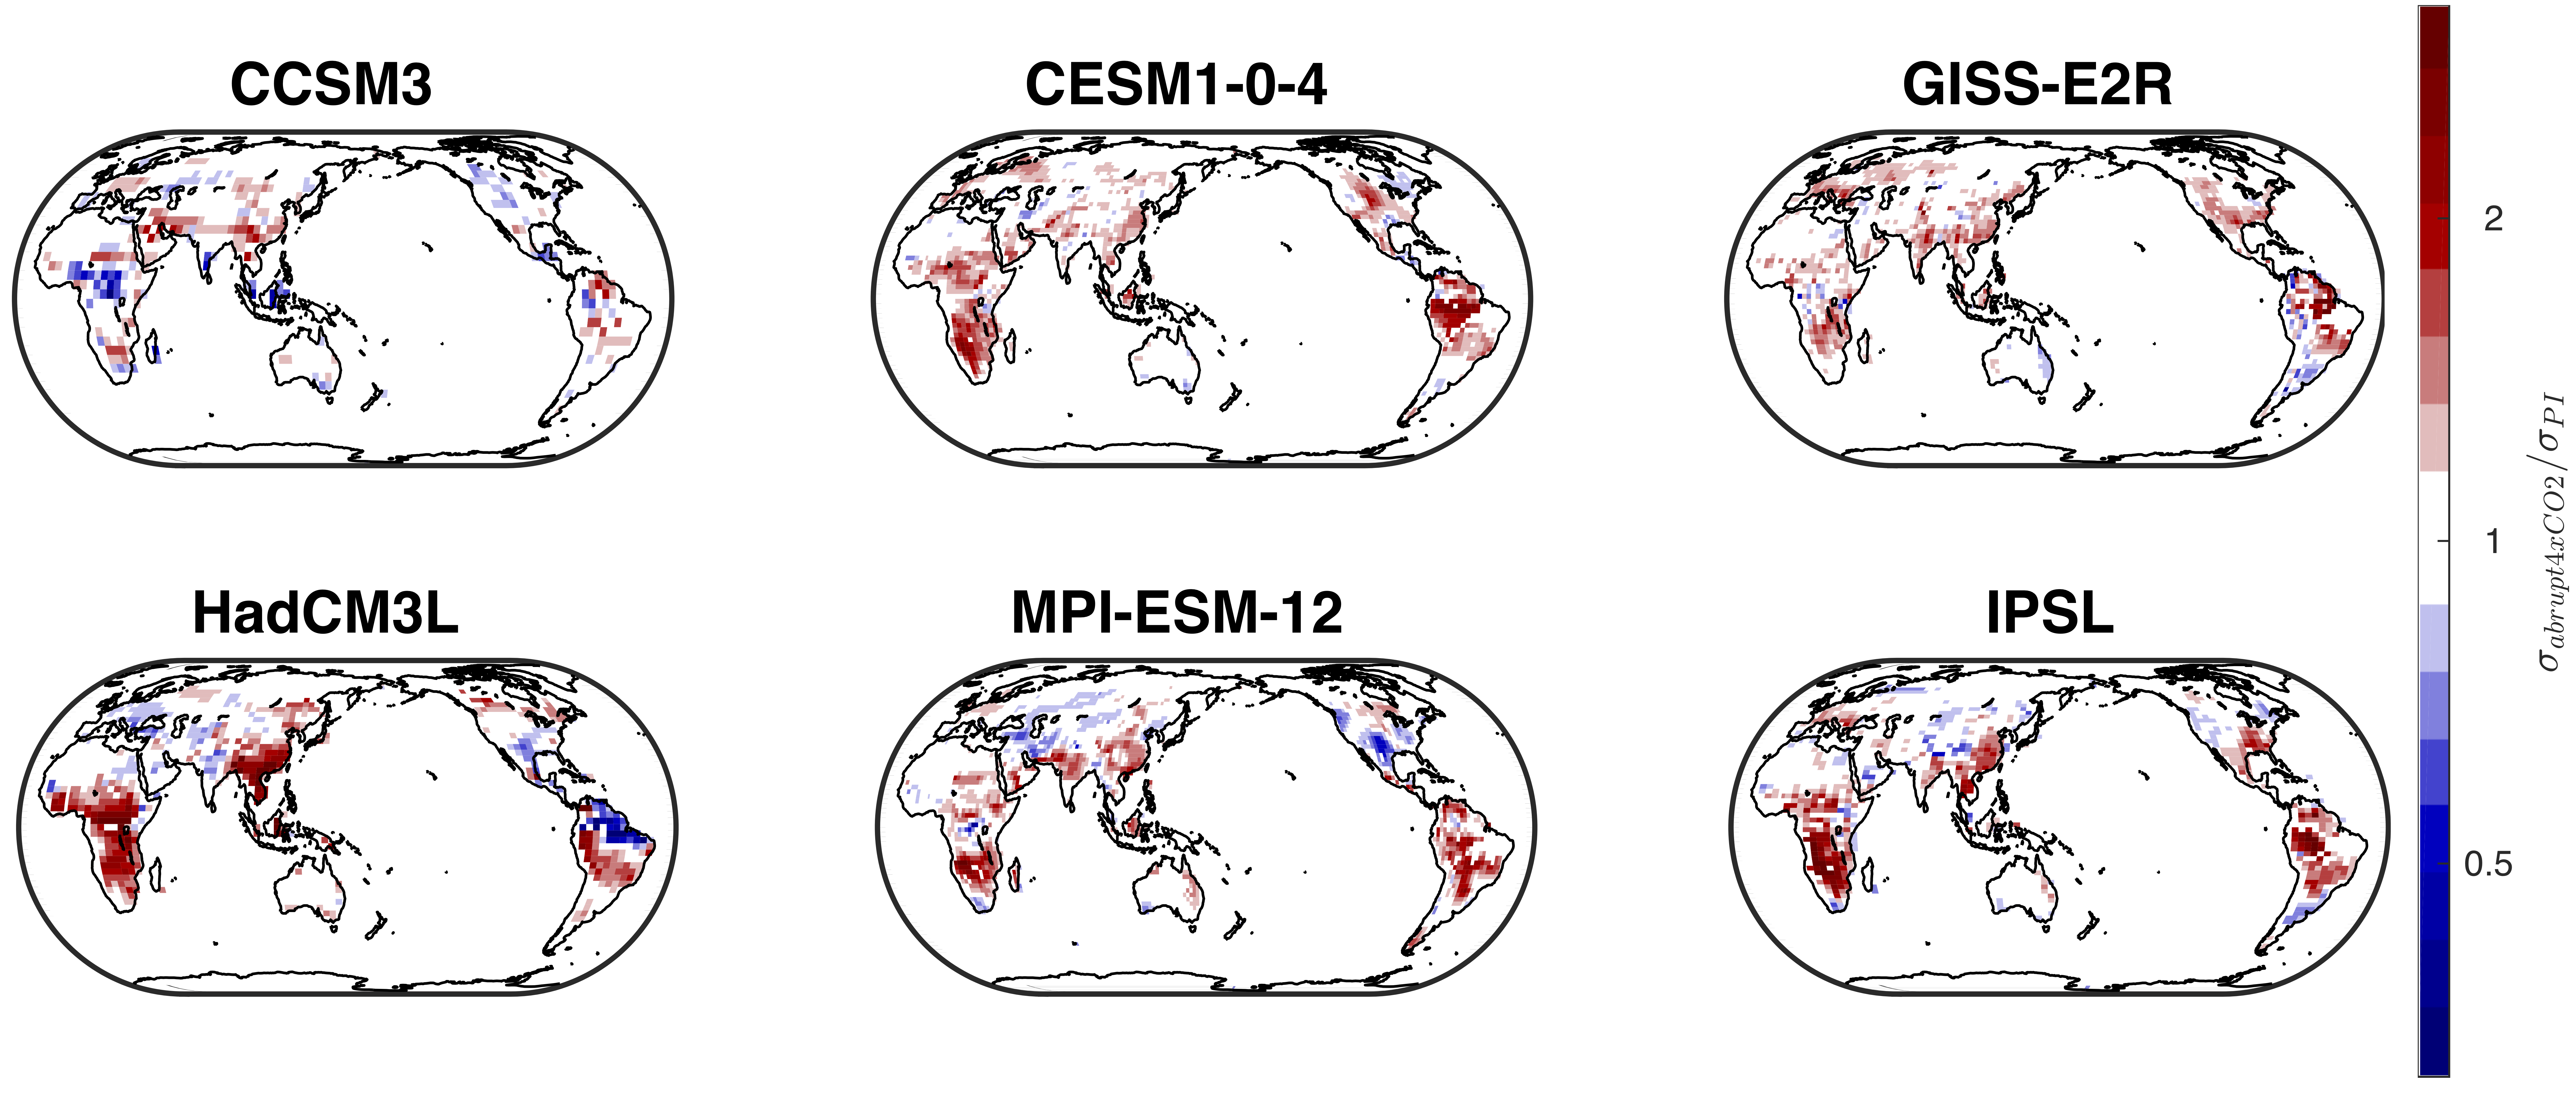
\includegraphics[width = 16.3cm]{tas_Amon_LRM6_abrupt4x_control_LF_maps_JJA_final.png}
  %\caption{
	  %Change in hemispheric-summer temperature variability for selected models in the CMIP-5 archive for an abrupt 4xCO$_2$ forcing. The heatmap shows the ratio in standard deviation in temperature  relative to preindustrial, using 30-year detrended timeseries \textcolor{red}{for future, XX-XX years after the forcing change}, for JJA (northern hemisphere) and DJF (southern hemisphere).  %\textcolor{red}{1981-2010 and 2071-2100} for JJA and DJF.
    %Blue indicates a decrease in variability and red an increase.
   %Climate models disagree about changes in variability, though most project slight increases during summer. The HadGEM2 model, used in examples here, exhibits relatively strong variability changes, with strong increases in Central and South America, East Asia, and Africa. 
	%\textcolor{red}{HadGEM2}.
  %}
	% XX EJM - need more numbers here, and should ideally change the plot so that the Pacific is not centered - instead center on land and cut the Pacific in half. If Ziwei cannot do this before submission time, OK to do it later.
	% HadCML has decreases in variability over N. America and Europe; would be  best to try again with another climate model - again can do after submission but be prepared to defend your assertions. It could be that the rice differences are because rice is grown in the places where varaibility increases
  %\label{fig:var}
%\end{figure}

\begin{figure}[h!]
  \centering
  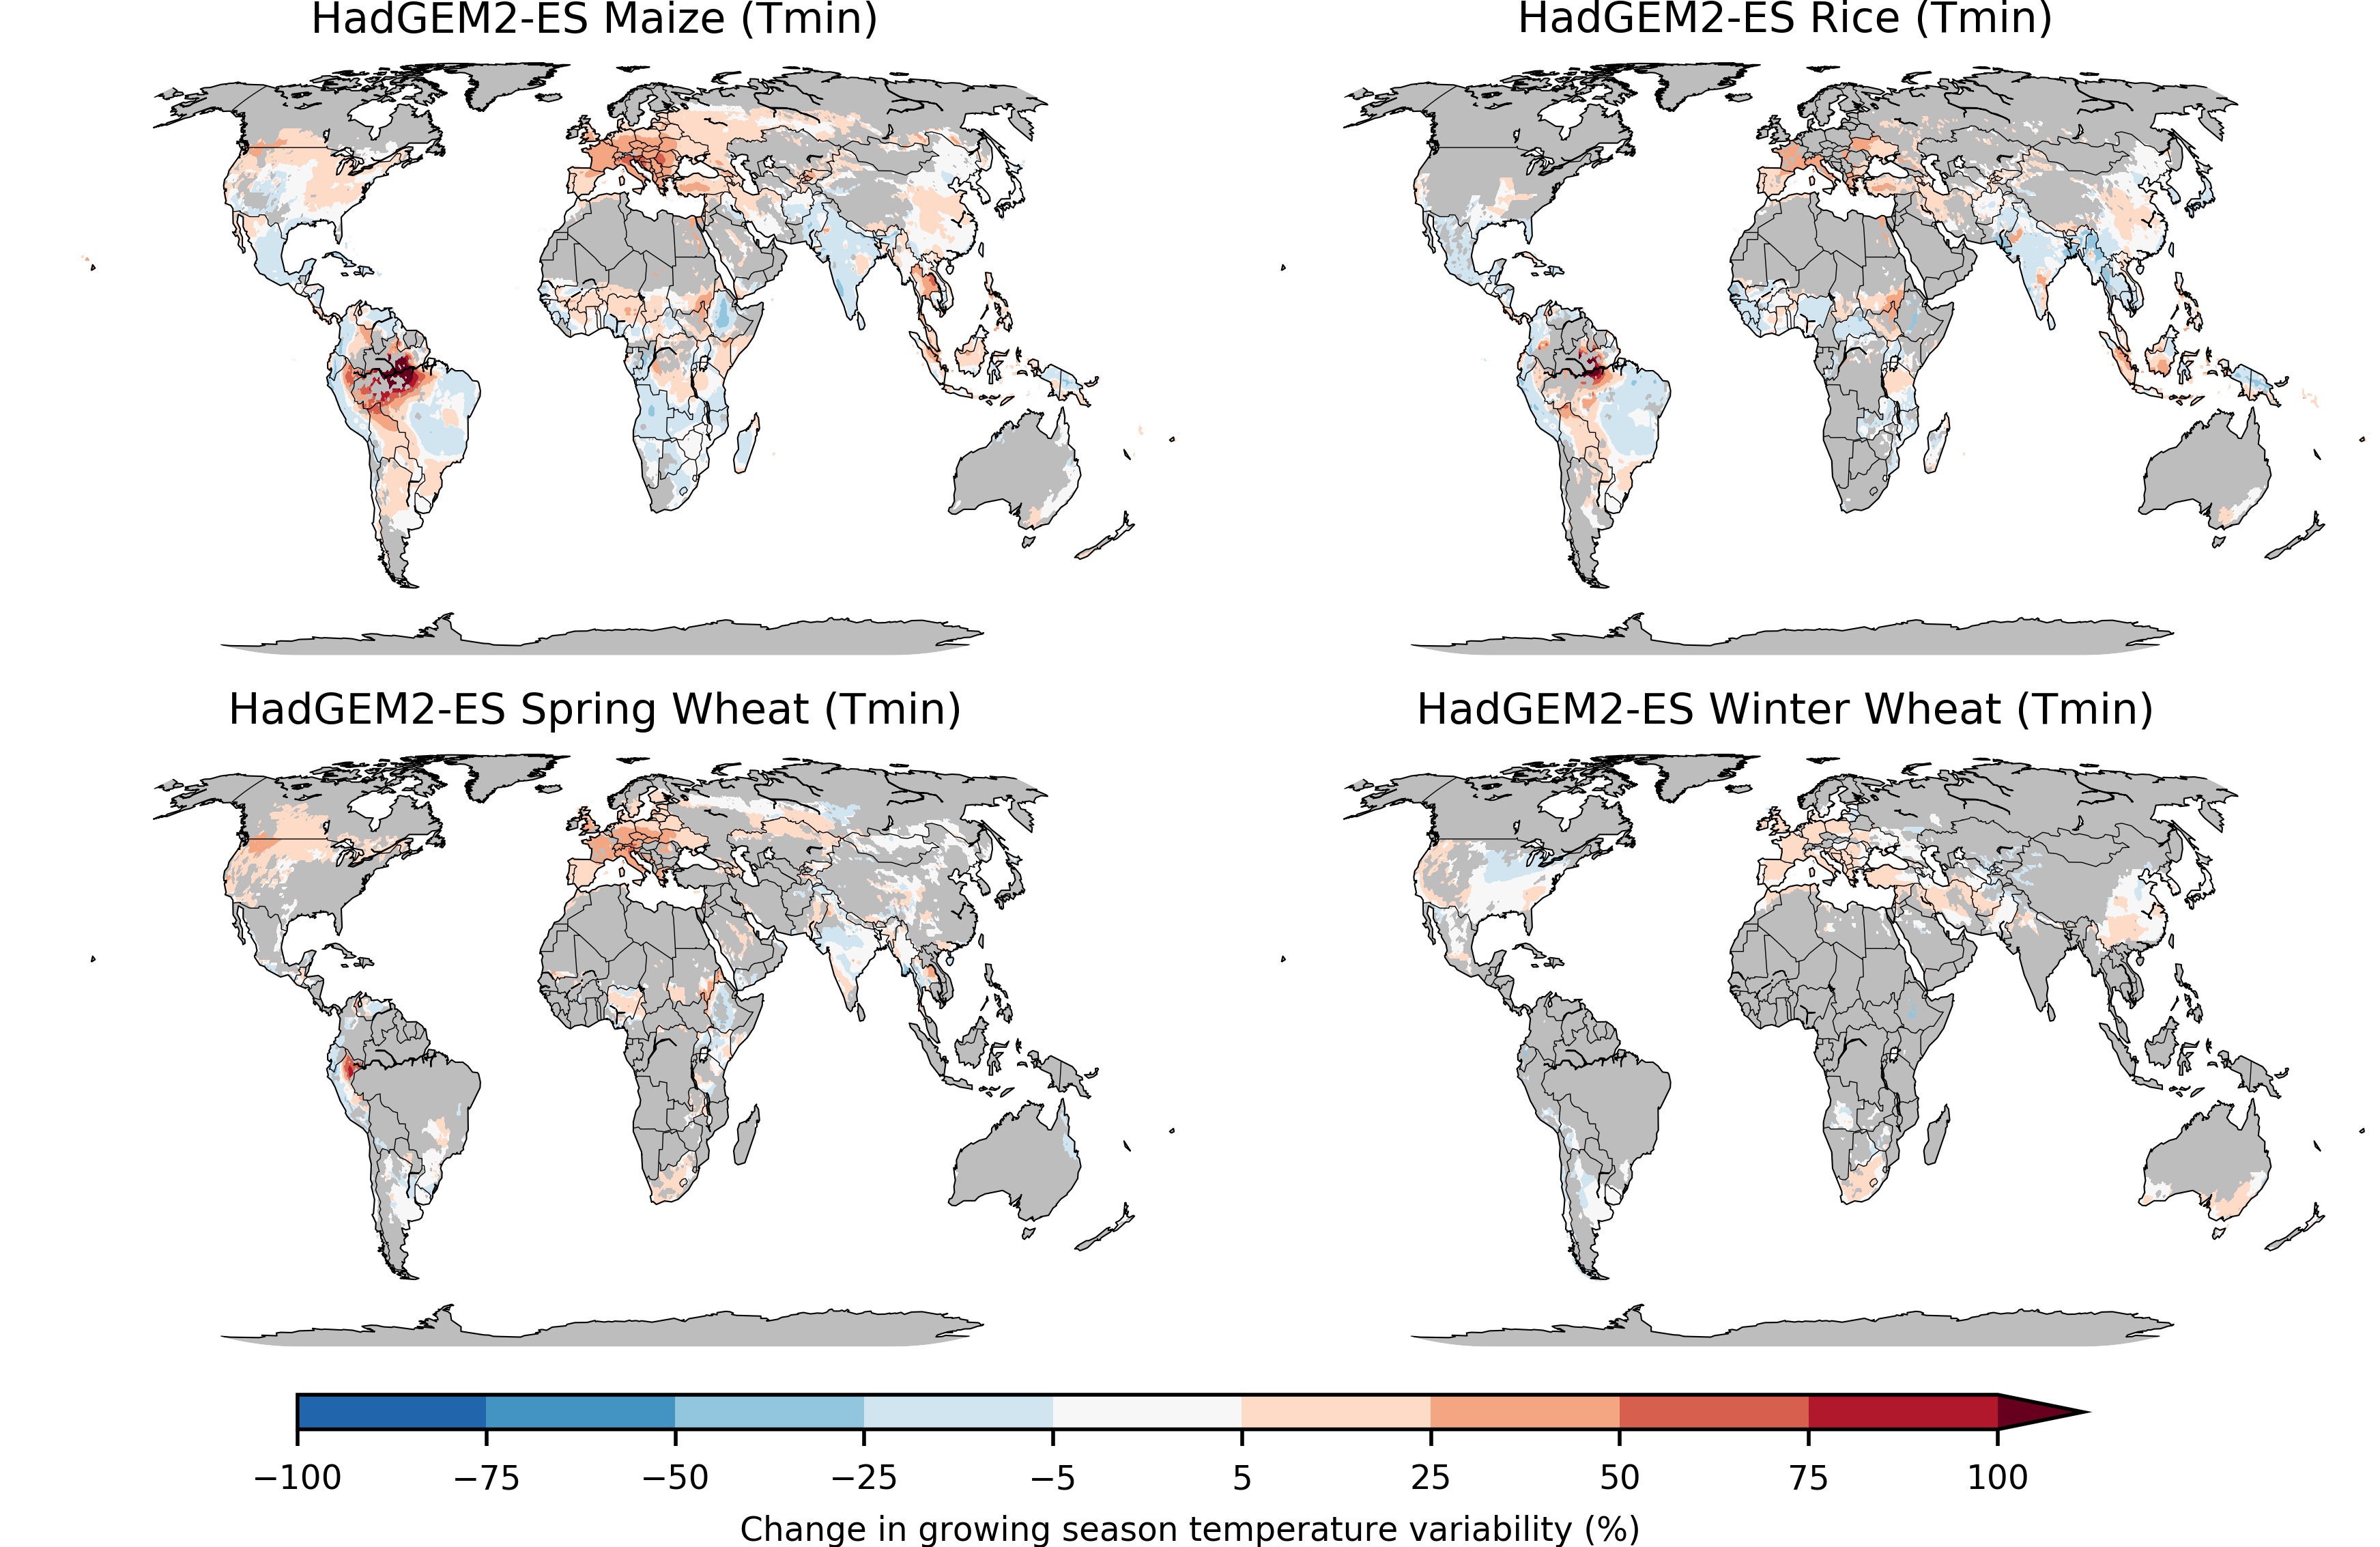
\includegraphics[width = 14cm]{HadGEM2-ES_var_change_min.png}
  \caption{
	  Change in within-growing-season daily minimum temperature variability by the end of century under RCP8.5 for the HadGEM2 model, computed for selected crops. 
	Heatmap shows the percentage change for 2070-2099 relative to 1981-2010 over currently cultivated areas, with red indicating increases and blue decreases. 
	To determine the change we compute the mean standard deviation of daily T$_{min}$ in each historical growing season and take the mean across all 30 years; this metric therefore includes changes both in seasonality and in short-term variations but excludes interannual variability and longer-term trends. For winter wheat, growing-season variability reductions reflect the dampening of the seasonal cycle (stronger warming in winter). 
	Strong percentage increases in the tropics reflect very low variability in the baseline. Production-weighted mean changes across crops range from -3\% for rice to +5\% for spring wheat (Table S1). Note that changes may differ if calculated using an ensemble of simulations rather than a single projection as is done here.
  }
  \label{fig:var}
\end{figure}

\begin{figure}[h!]
  \centering
  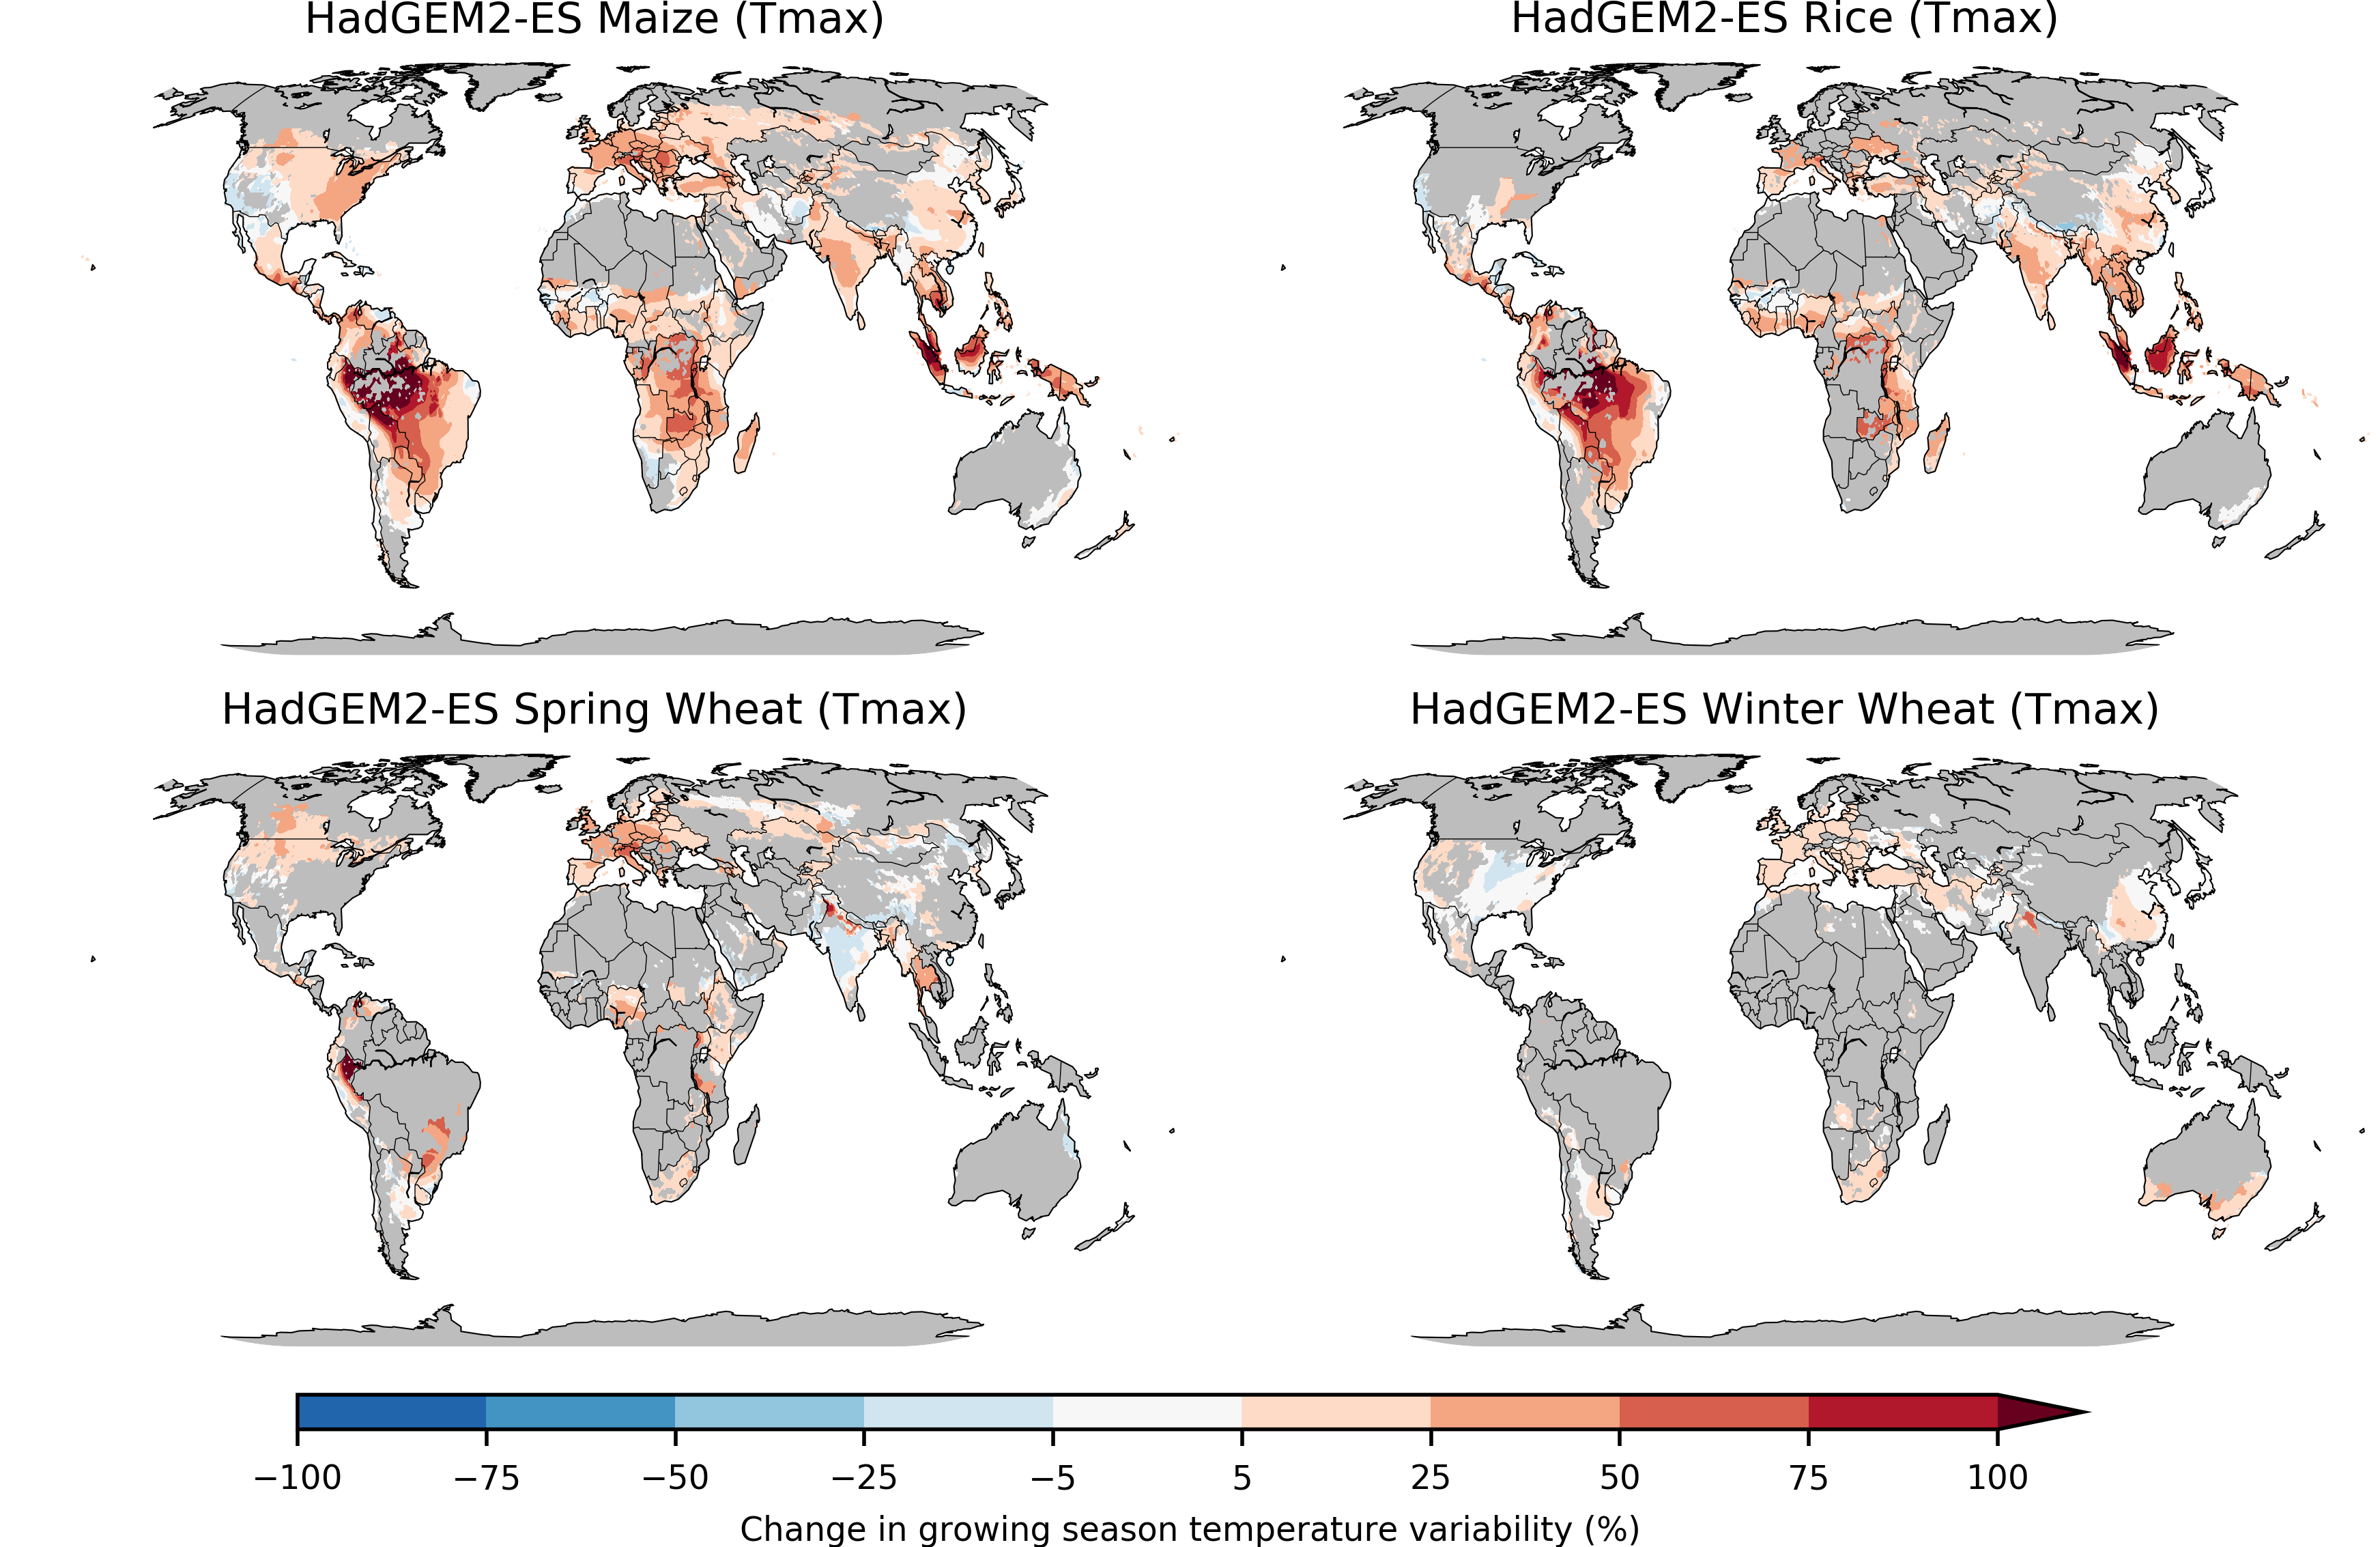
\includegraphics[width = 14cm]{HadGEM2-ES_var_change_max.png}
  \caption{
  As in Figure S3 except now for daily maximum temperature. Changes in daily maximum temperature variability are generally more positive than those for daily minimum temperature.
  }
  \label{fig:var}
\end{figure}

\begin{figure}[h!]
  \centering
  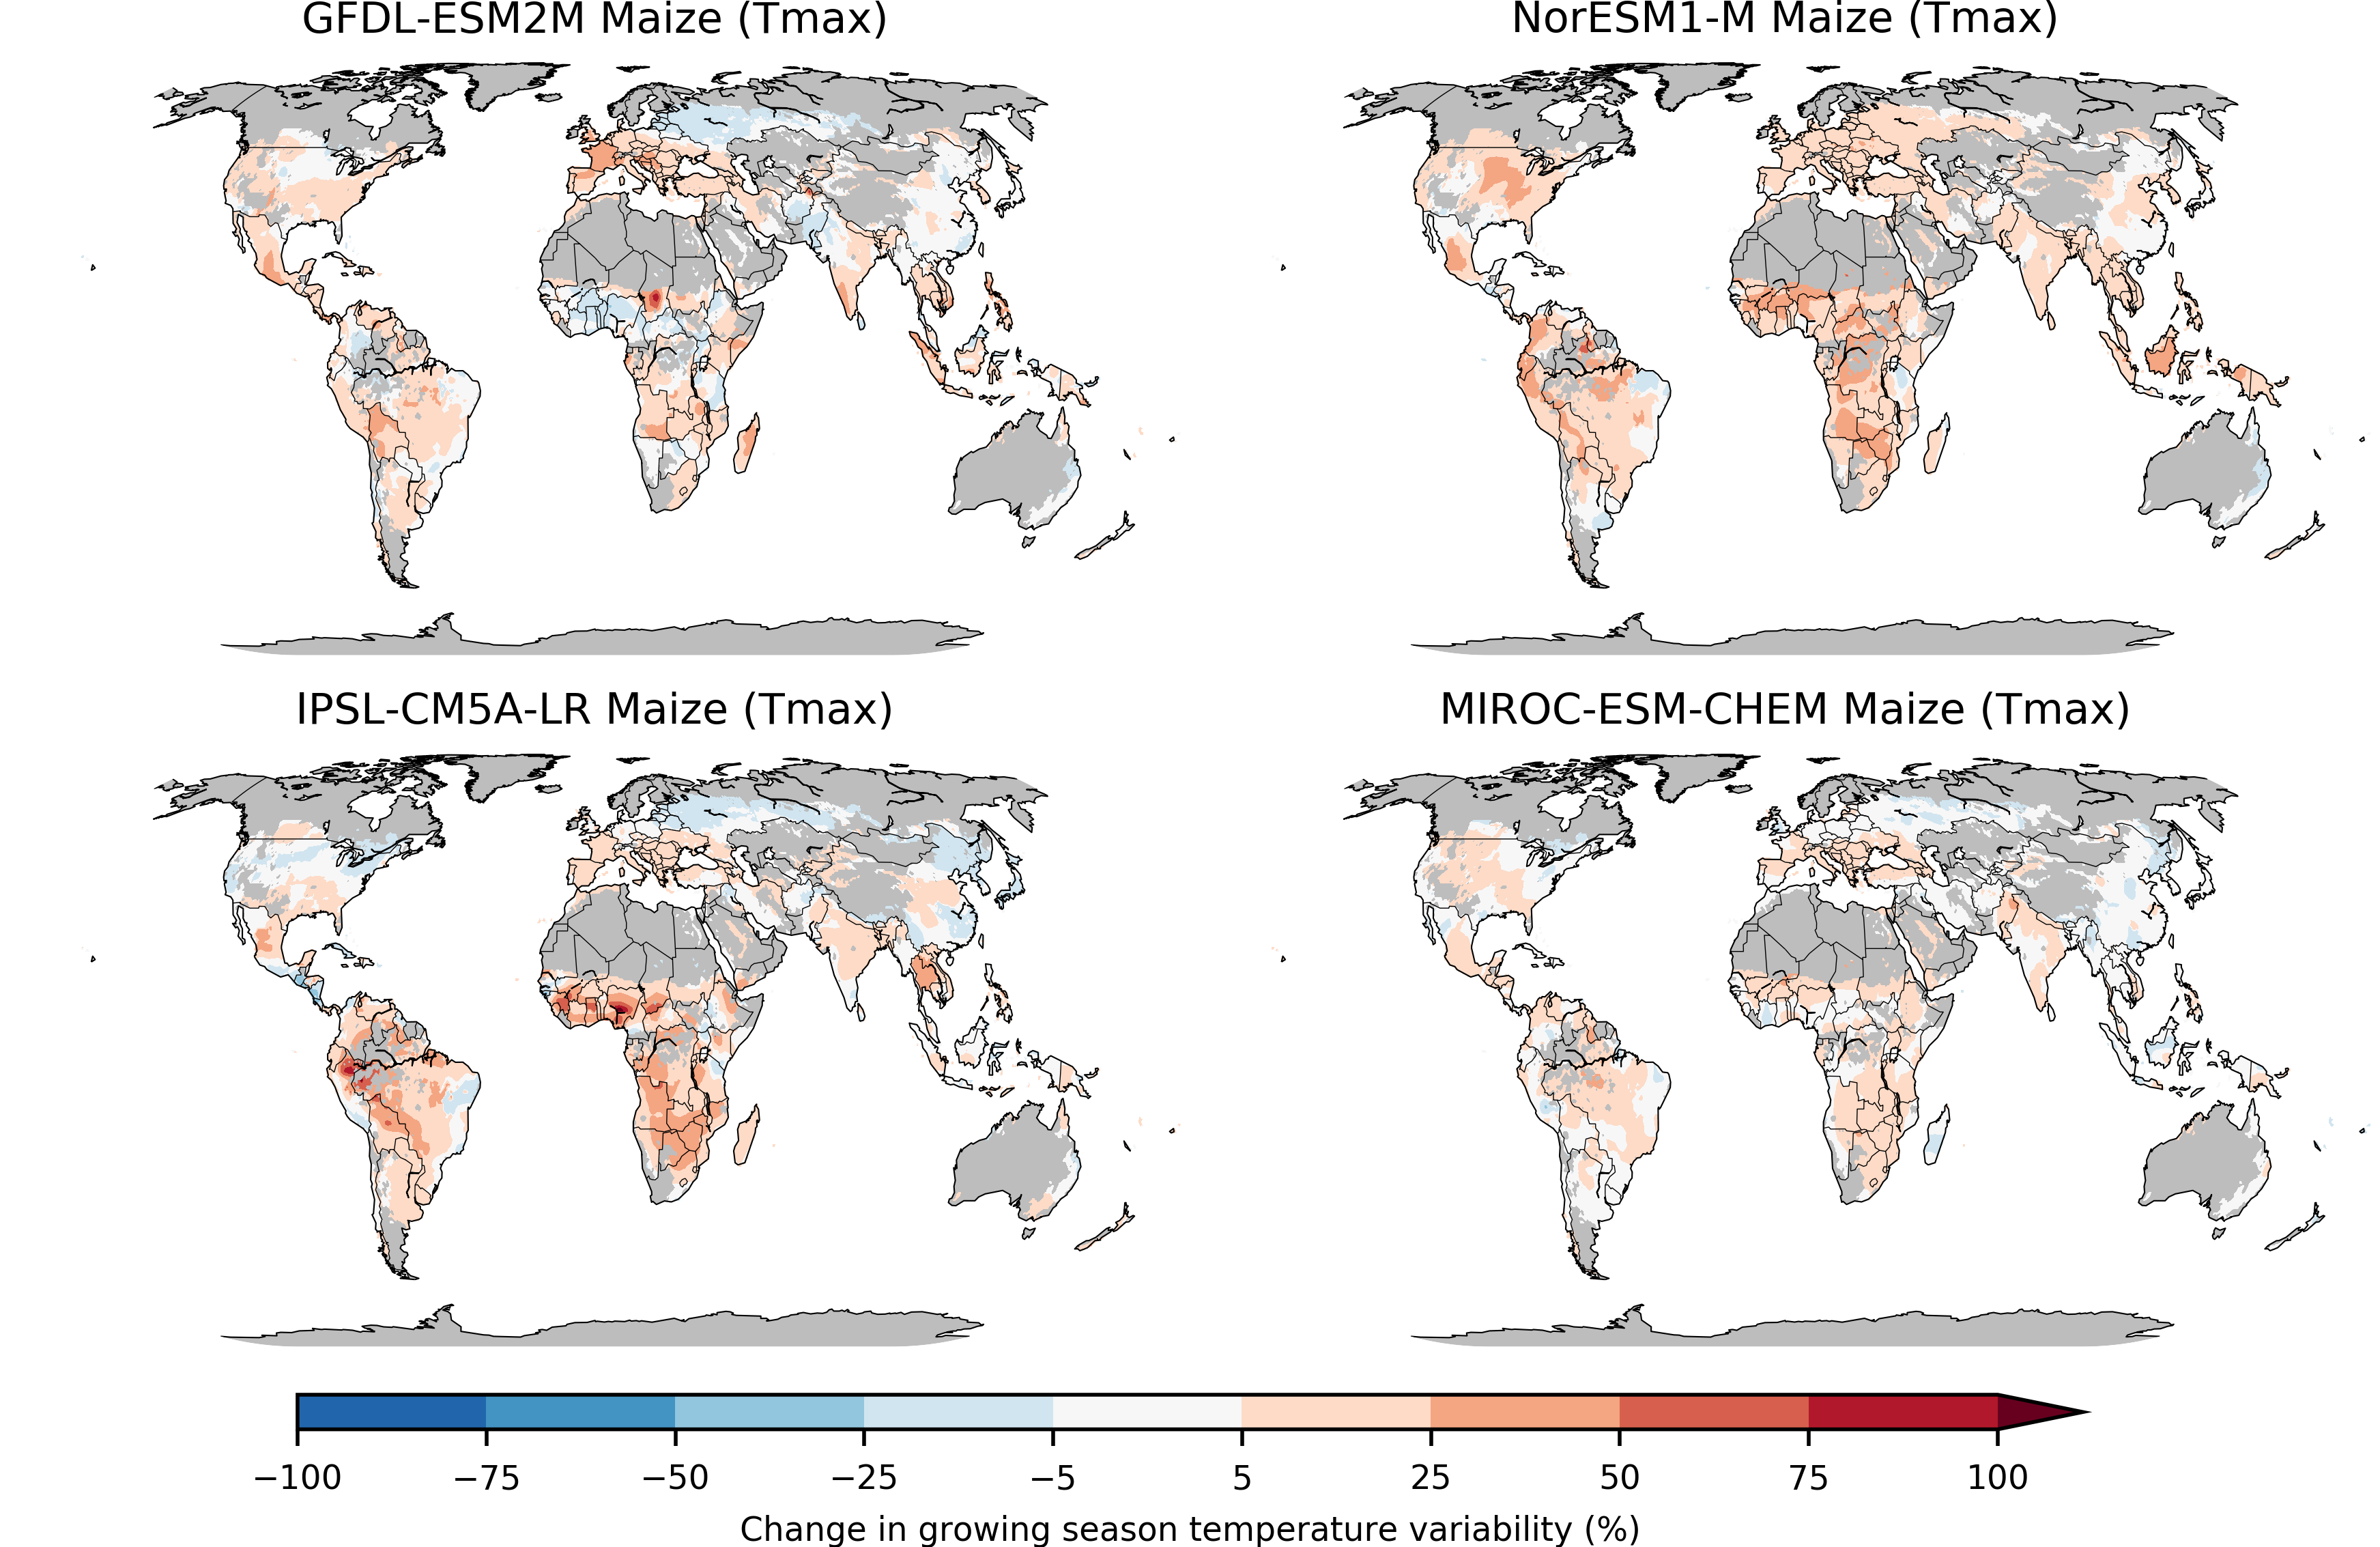
\includegraphics[width = 14cm]{other_models_var_change_max.png}
  \caption{
  As in Figure S4, change in daily maximum temperature variability, except now for maize only, for the remaining 4 ISIMIP climate simulations. Values are lower on average than for HadGEM2-ES but patterns can differ.
  }
  \label{fig:var}
\end{figure}


%%%%%%%%%%%%%%%%%%%%%%%%%%%%%%%%%%%%%%%%%%%%%%%%%%%%%%%%%%%%%%%%%%%%%%%%%%%%%%%%%%%%%%%
%%%%%%%%%%%%%%%%%%%%%%%%%%%%%%%%%%%%%%%%%%%%%%%%%%%%%%%%%%%%%%%%%%%%%%%%%%%%%%%%%%%%%%%
%%%%%%%%%%%%%%%%%%%%%%%%%%%%%%%%%%%%%%%%%%%%%%%%%%%%%%%%%%%%%%%%%%%%%%%%%%%%%%%%%%%%%%%
\clearpage
\section{Yield response for A1 (growing season adaptation) simulations}
\begin{justify}
	This section shows illustrations of emulator ability to capture yield changes in A1 simulations; compare to main text Figures 5 and 6 showing A0 simulations. Responses to CWN factors are similar in both but responses to T are substantially weaker in A1 simulations, in which growing season length does not contract in warmer future conditions.
\end{justify}

\begin{figure}[h!]
\centering
    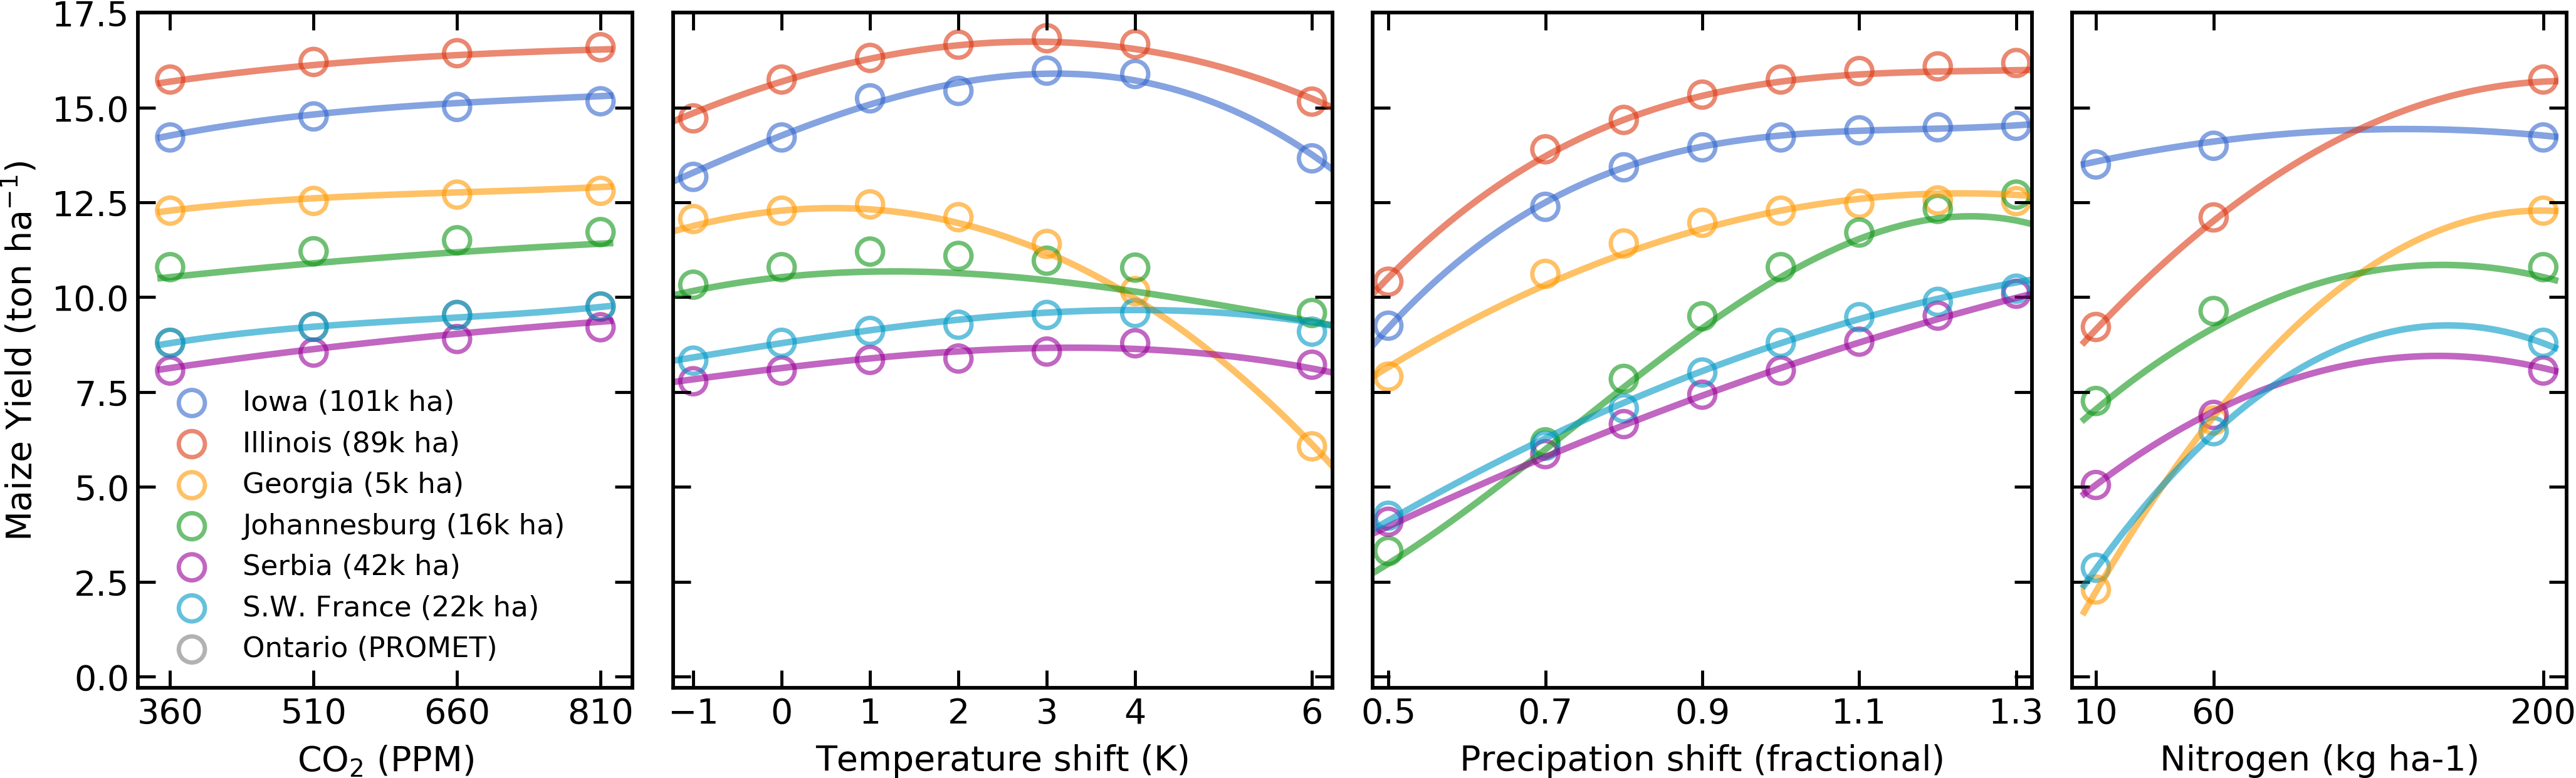
\includegraphics[width=16.3cm]{regression_exampleA1.png}
    \caption{
    Illustration of spatial variations in yield response, which are successfully captured by the emulator for the A1 simulations. 
    Panels show simulations (points) and emulations (lines) of rainfed maize in the pDSSAT model in six example locations selected to represent high-cultivation areas around the globe. 
    Legend includes hectares cultivated in each selected grid cell. 
    Each panel shows variation along a single variable, with others held at baseline values. 
    }
   \label{fig:regression}
\end{figure}

\begin{figure}[h!]
\centering
    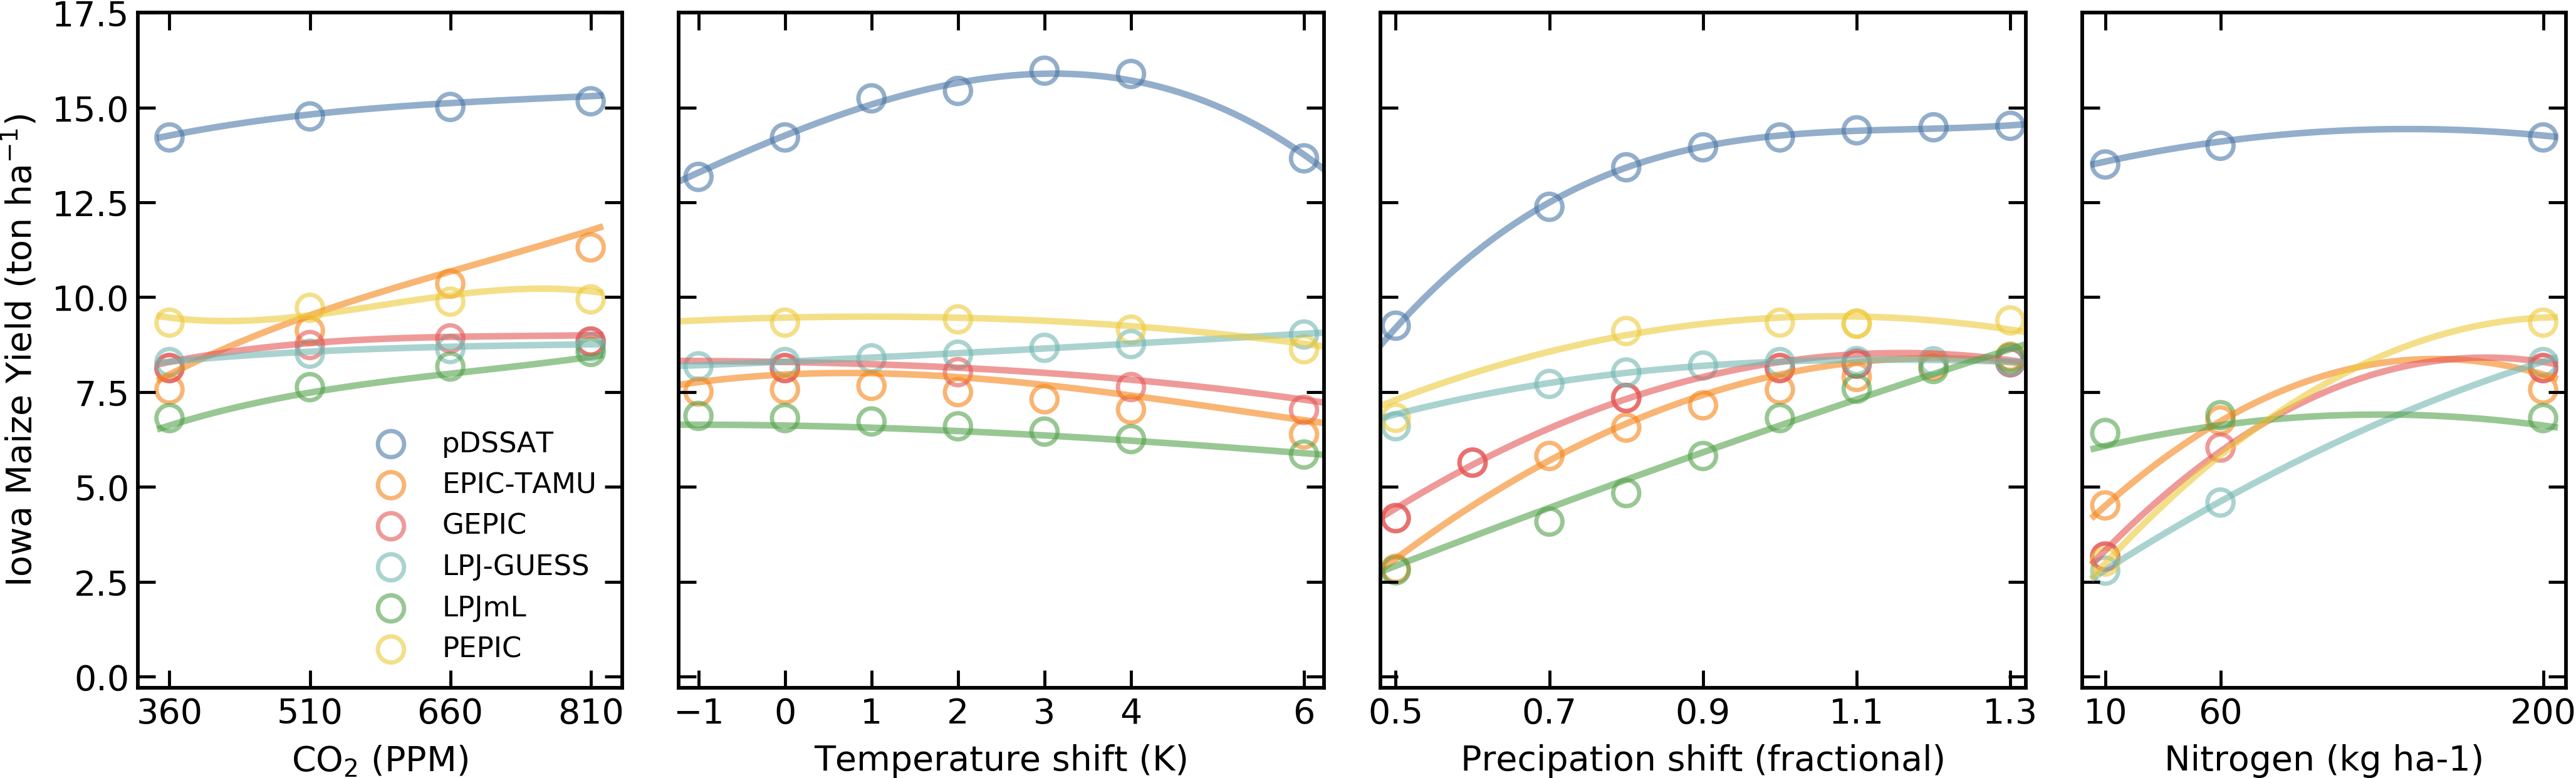
\includegraphics[width=16.3cm]{regression_exampleA1_2.png}
    \caption{
    Illustration of variations in yield response across models for A1 simulations, again successfully captured by the emulator. 
    Panels show simulations and emulations from six representative GGCMI models for rainfed maize in the same Iowa grid cell shown above, with the same plot conventions. 
    Three models (PROMET, JULES, and CARAIB) that do not simulate the nitrogen dimension are omitted for clarity. 
    }
   \label{fig:regression_2}
\end{figure}

%%%%%%%%%%%%%%%%%%%%%%%%%%%%%%%%%%%%%%%%%%%%%%%%%%%%%%%%%%%%%%%%%%%%%%%%%%%%%%%%%%%%%%%
%%%%%%%%%%%%%%%%%%%%%%%%%%%%%%%%%%%%%%%%%%%%%%%%%%%%%%%%%%%%%%%%%%%%%%%%%%%%%%%%%%%%%%%
%%%%%%%%%%%%%%%%%%%%%%%%%%%%%%%%%%%%%%%%%%%%%%%%%%%%%%%%%%%%%%%%%%%%%%%%%%%%%%%%%%%%%%%

\clearpage
\section{Normalized error for other cases}
\begin{justify}
In manuscript Figure 7 we show normalized error for the A0 emulators over all rainfed crops, models, and T and W values for 
	baseline CO$_2$ and nitrogen levels (360 ppm and 200 kg ha-1). Here we show normalized error in some alternate cases for comparison: \textit{Figure S6:} A0 emulators of rainfed crops at higher CO$_2$, \textit{Figure S7:} A1 emulators of rainfed crops at baseline values, \textit{Figure S8):} A0 emulators of irrigated crops at 
baseline values. 
Results are generally similar, with a few exceptions. Normalized errors at higher CO$_2$ are generally lower because model disagreement is larger, lowering the denominator. Some model emulators for irrigation water demand are under-performing: LPJ-GUESS and CARAIB for some crops.
A1 errors are larger than A0 errors for several crops and models: LPJmL rice, pDSSAT spring wheat, and PROMET winter wheat.
\end{justify}

\vspace{1in}

\begin{figure}[h!]
  \centering
  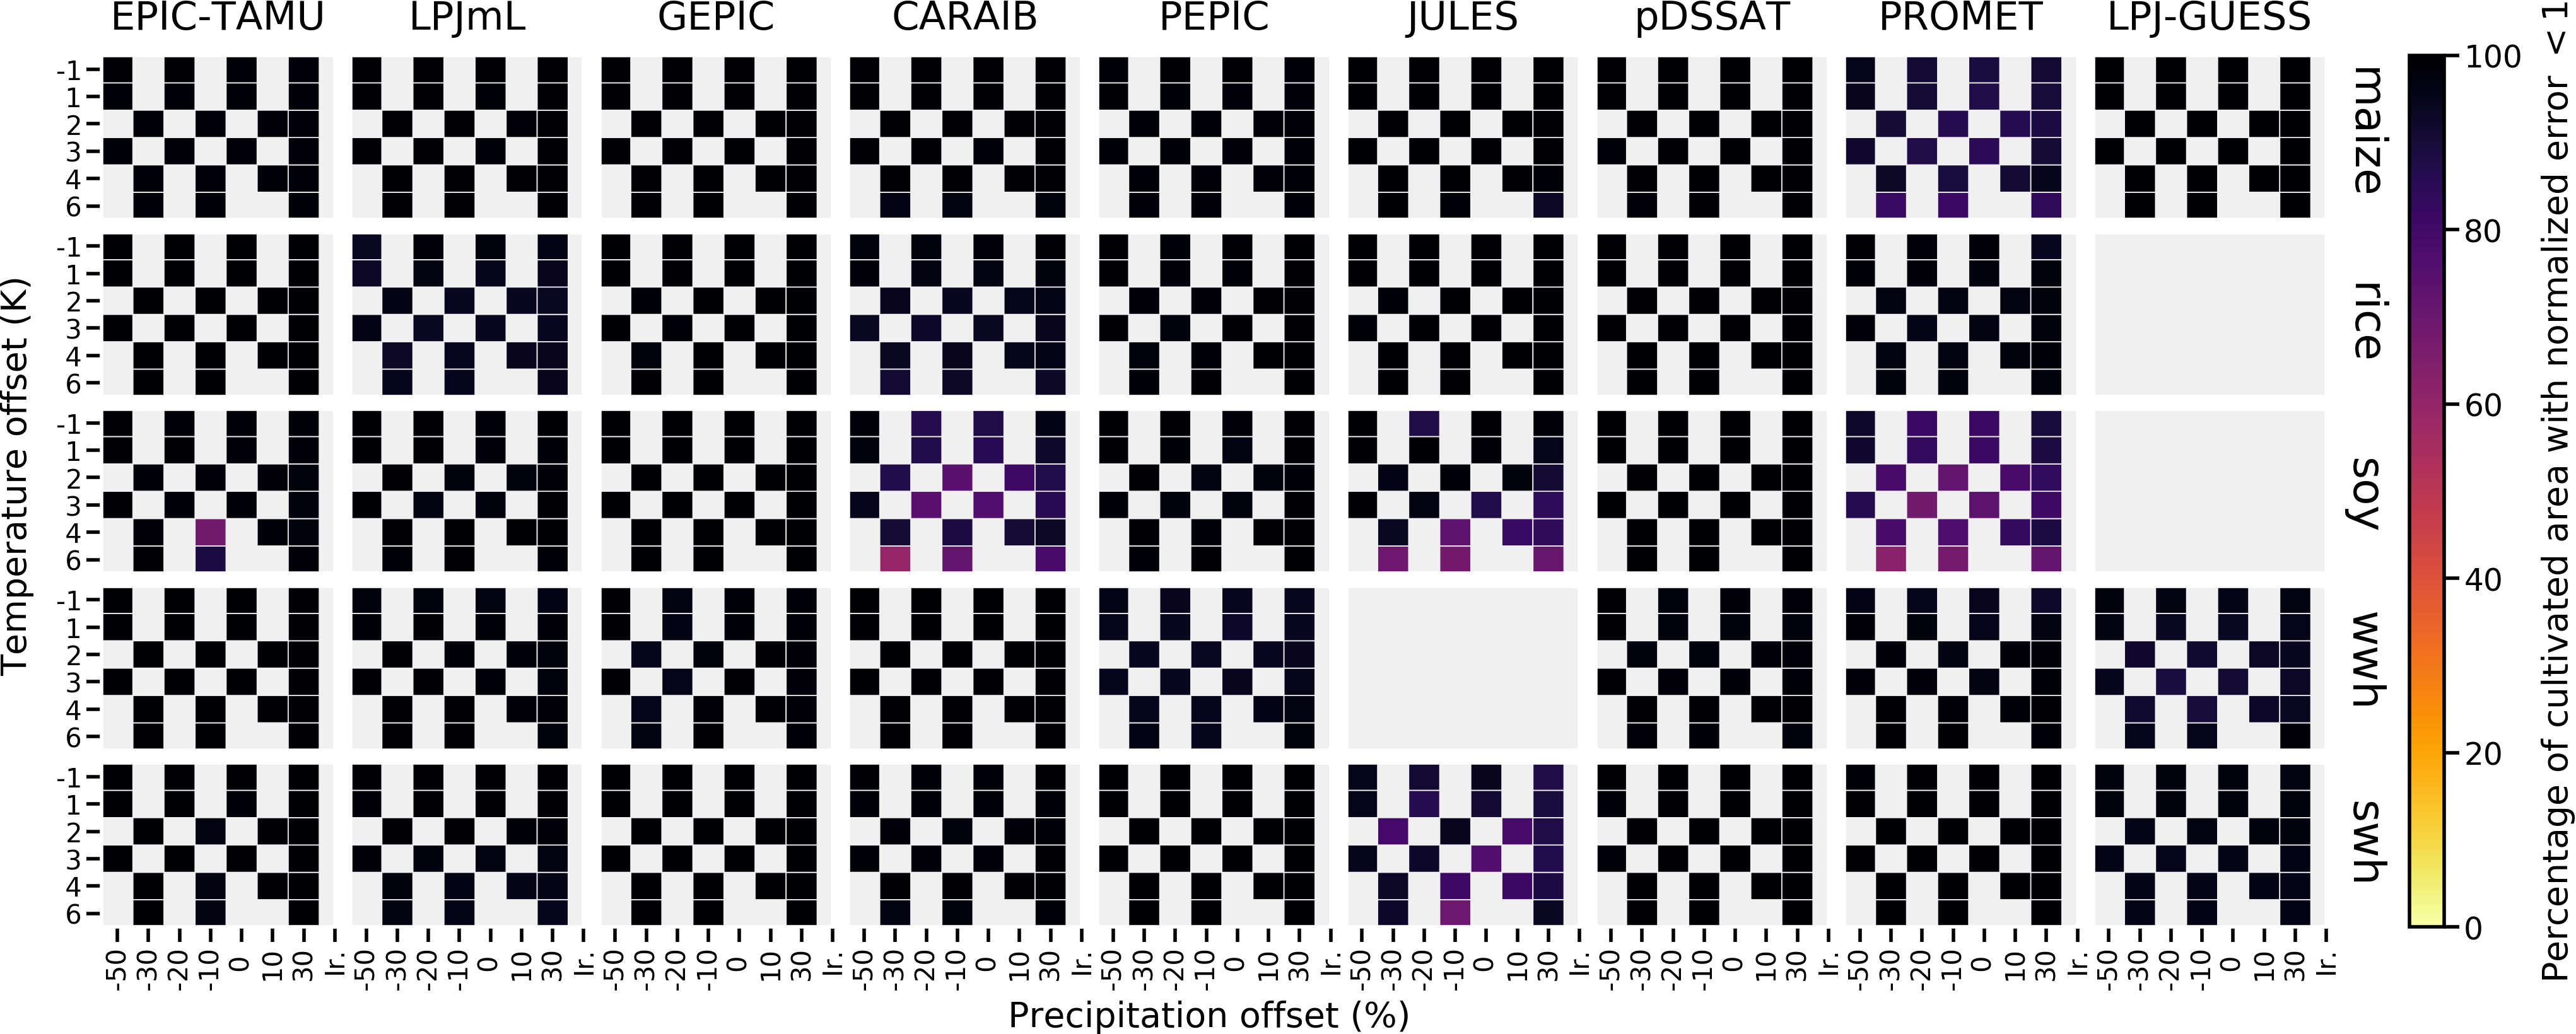
\includegraphics[width=15.5cm]{error_grid_810.png}
  \caption{
  Fraction of currently cultivated hectares with normalized emulation error less than 1 for the CO$_2$=810 ppm and 200 kg~N ha$^{-1}$ yr$^{-1}$ case for the temperature and precipitation perturbations scenarios provided by all 9 models included in the emulator analysis. 
  Figure convention as in main text Figure 7.
  The yield response is generally easy to emulate over currently cultivated areas (black regions).
  }
  \label{fig:error810}
\end{figure}

\begin{figure}[h!]
  \centering
  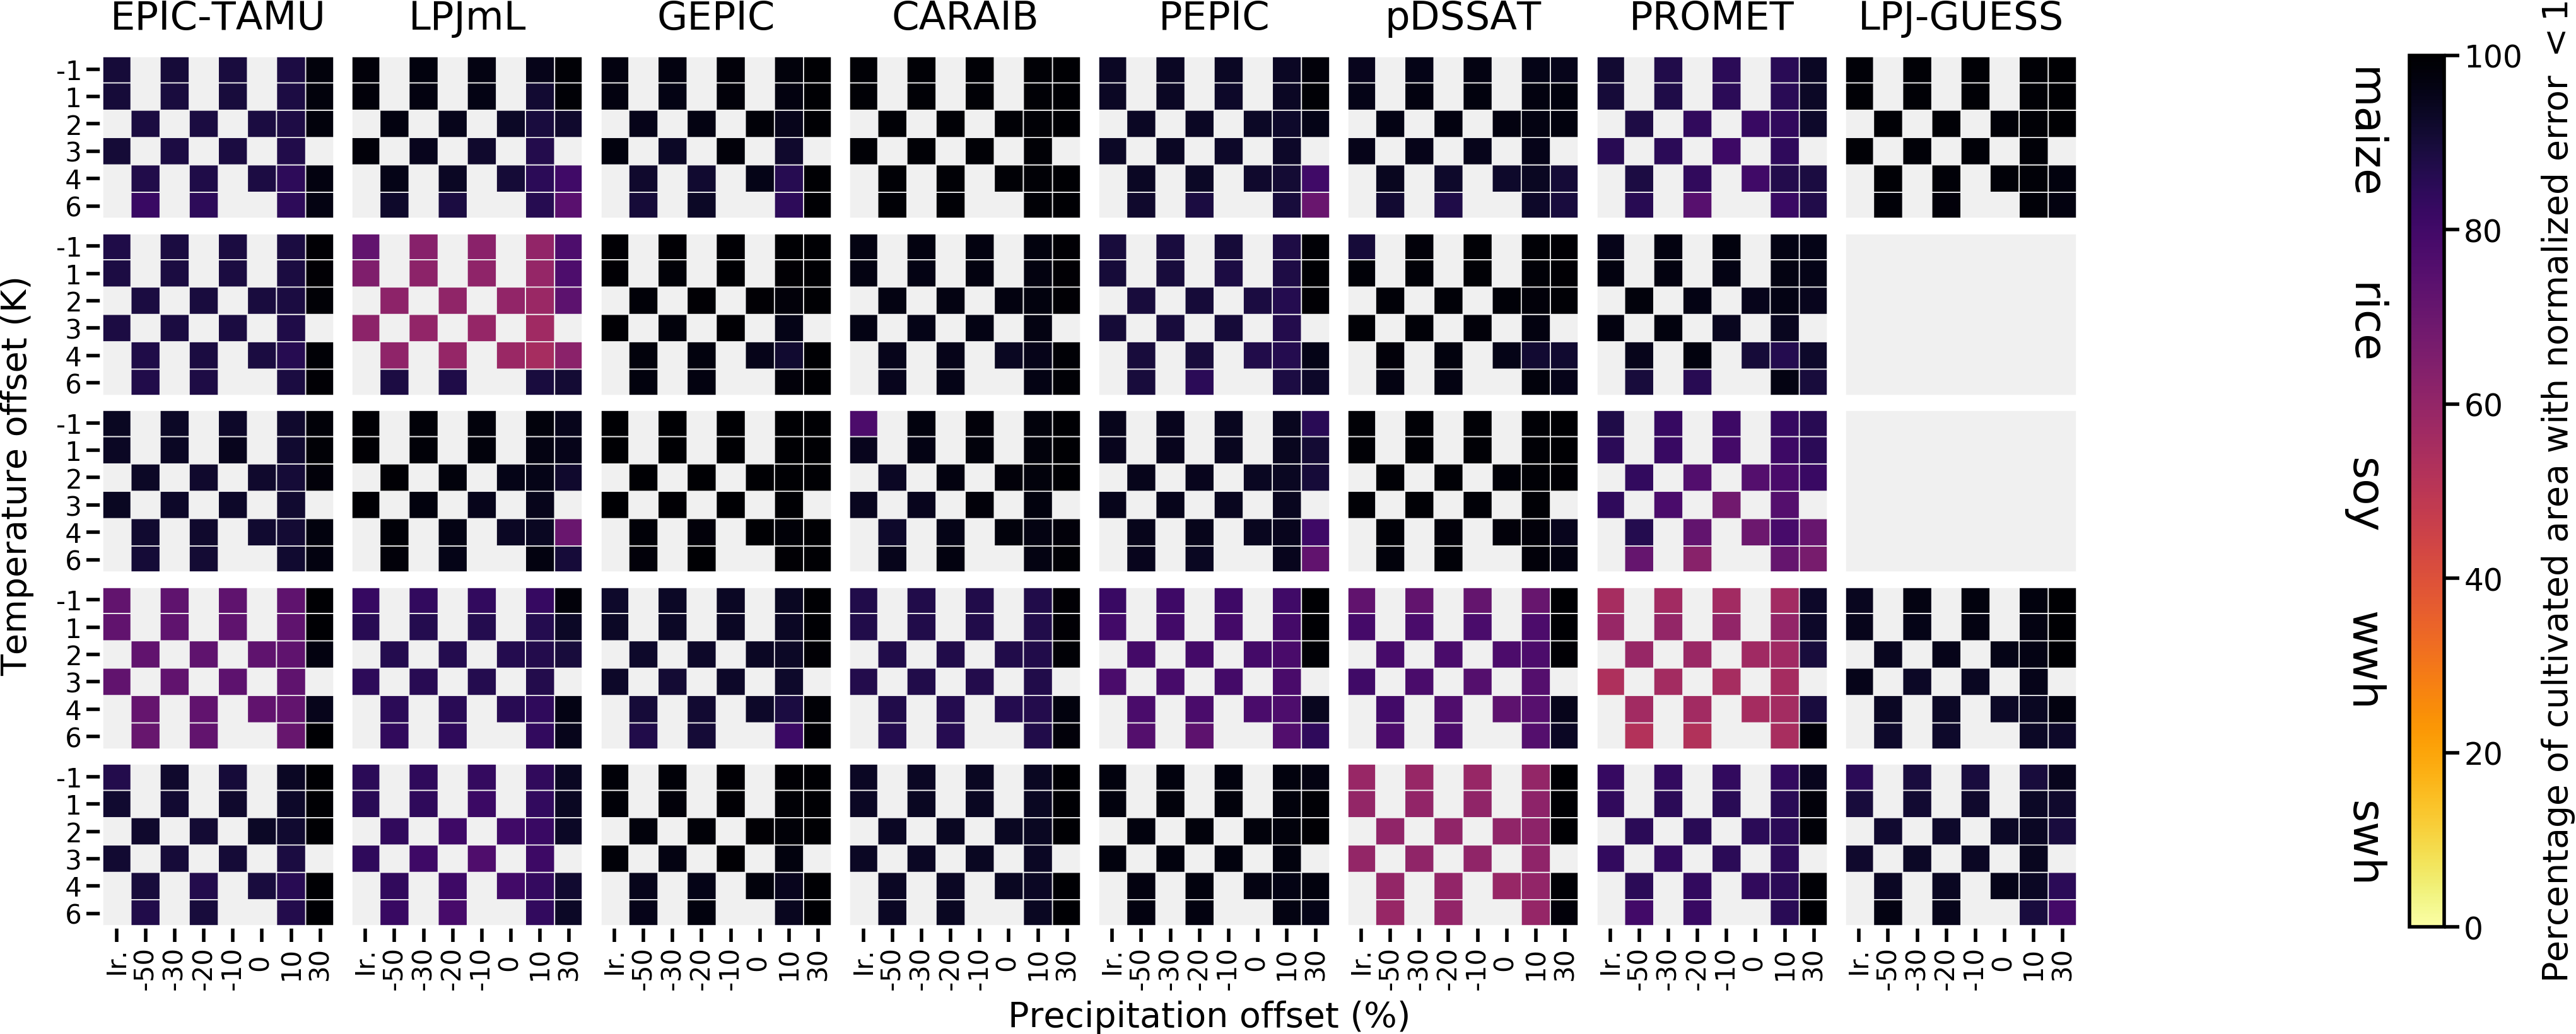
\includegraphics[width=15.5cm]{error_grid_360_cultivated_A1.png}
  \caption{
  Fraction of currently cultivated hectares with normalized emulation error less than 1 for A1 yield emulation for CO$_2$=310 ppm and 200 kg~N ha$^{-1}$ yr$^{-1}$ case. Figure convention as in main text Figure 7.
  }
  \label{fig:error810}
\end{figure}

\begin{figure}[h!]
  \centering
  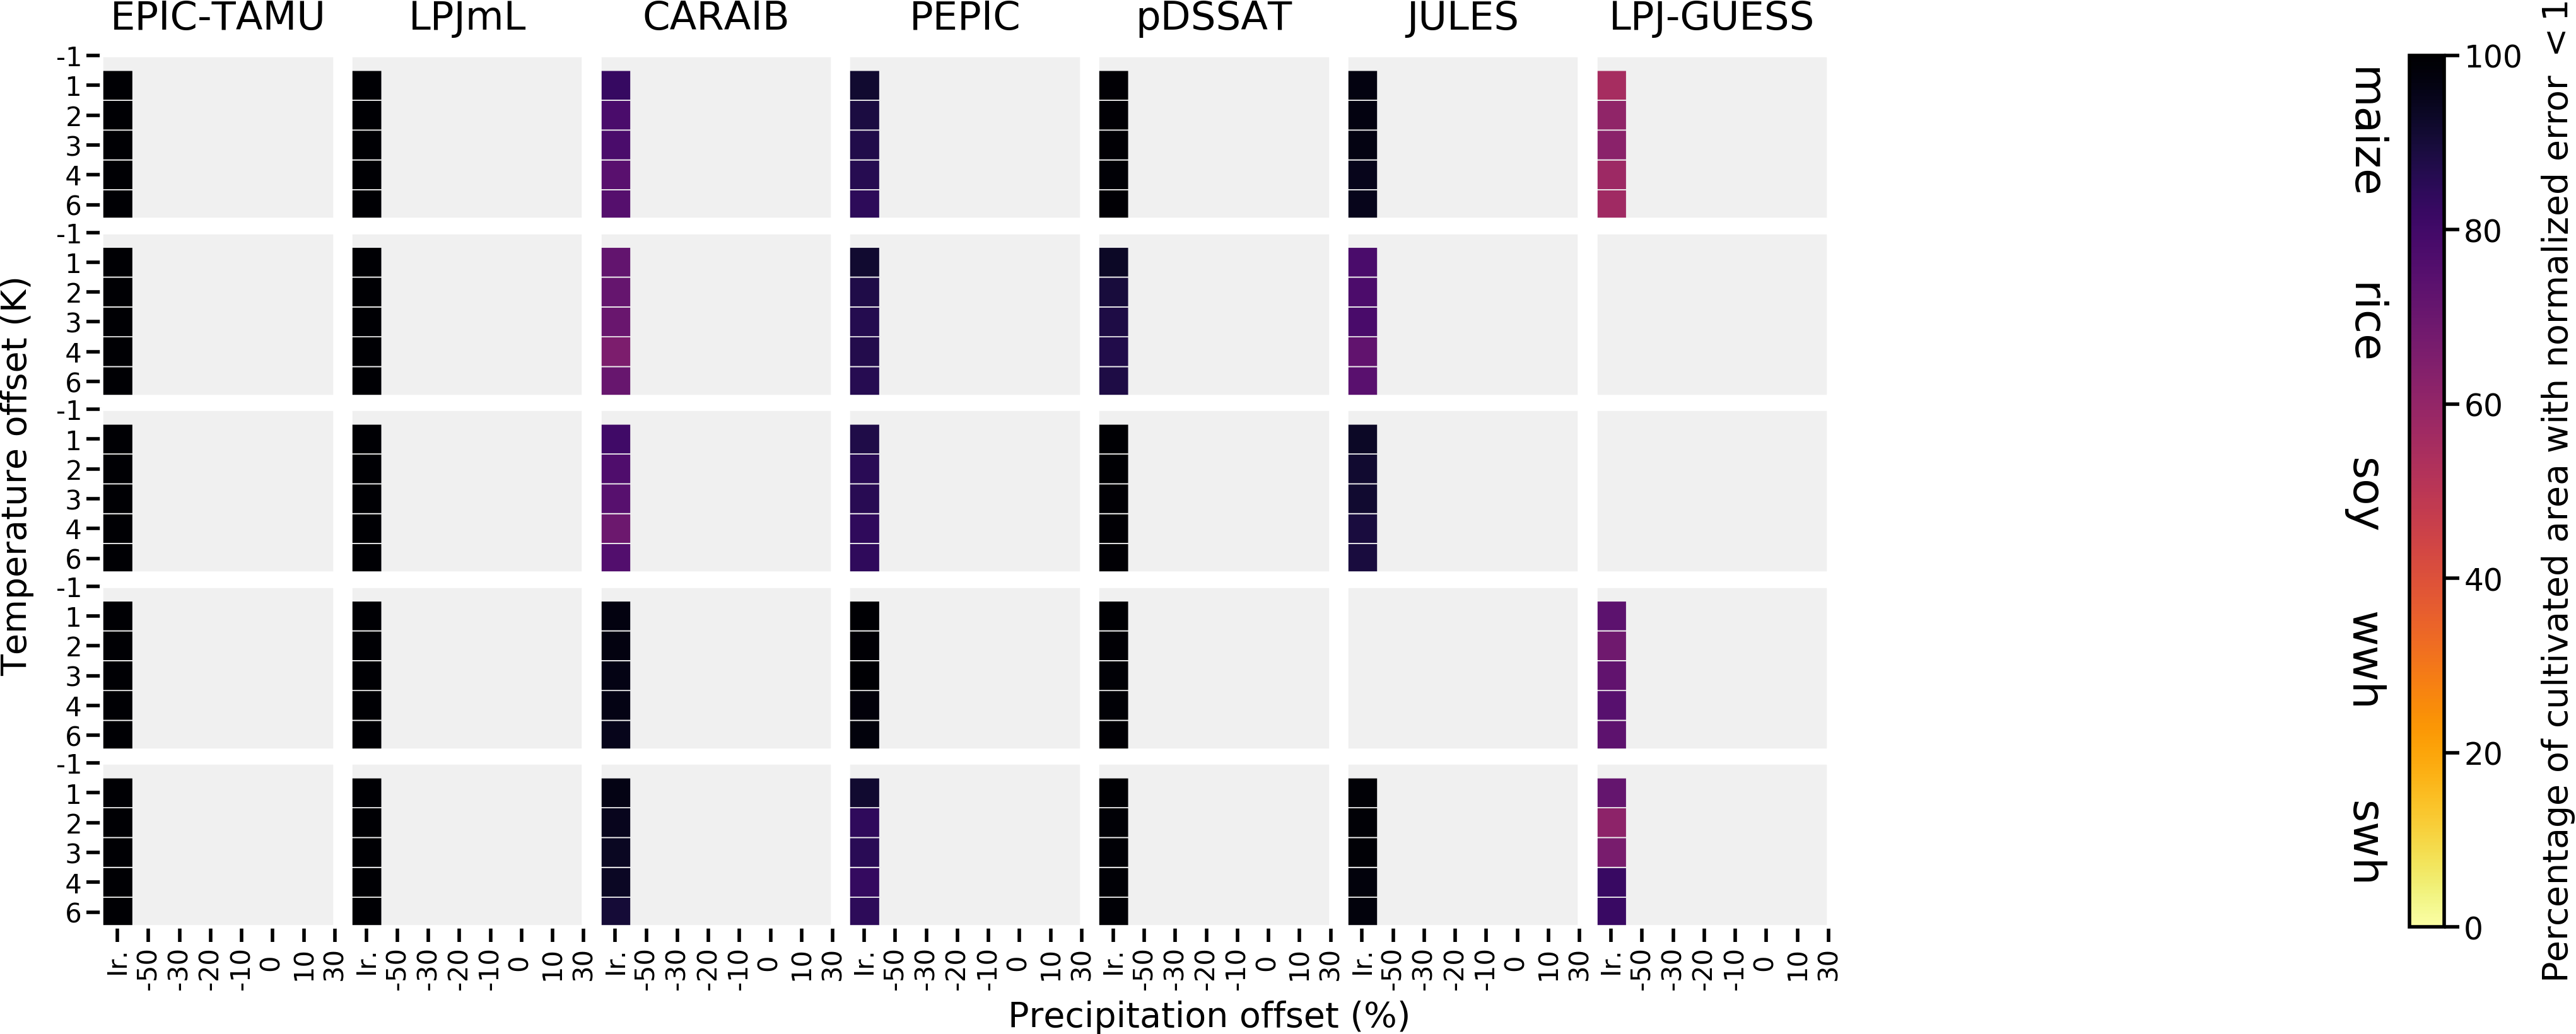
\includegraphics[width=15.5cm]{error_grid_360_cultivated_IWD.png}
  \caption{
  Fraction of currently cultivated hectares with normalized emulation error less than 1 for irrigated water demand emulation for CO$_2$=310 ppm and 200 kg~N ha$^{-1}$ yr$^{-1}$ case. Figure convention as in main text Figure 7.
  }
  \label{fig:error810}
\end{figure}

\clearpage
\section{Emulation of yields in a realistic climate simulation at high latitude}
\begin{justify}
In manuscript Section 4.3 we test the emulator against crop model simulations driven by a more realistic future climate projection to evaluate the impact of future variability changes that are not captured by the emulator. 
	Figure \ref{fig:lpjmlrcp} below isolates the mid- and high latitudes; compare to manuscript Figure 9 that shows global currently cultivated land. 
	Results are generally unchanged by the restriction in latitude except for rice, which is typically grown in tropics and subtropics: only 20\% of global rice production is grown north of 30N and 1\% north of 45N, with even less in the Southern hemisphere, only 0.8\%  south of 30S and none south of 45S.
\end{justify}

\vspace{0.5in}
\begin{figure}[h!]
  \centering
  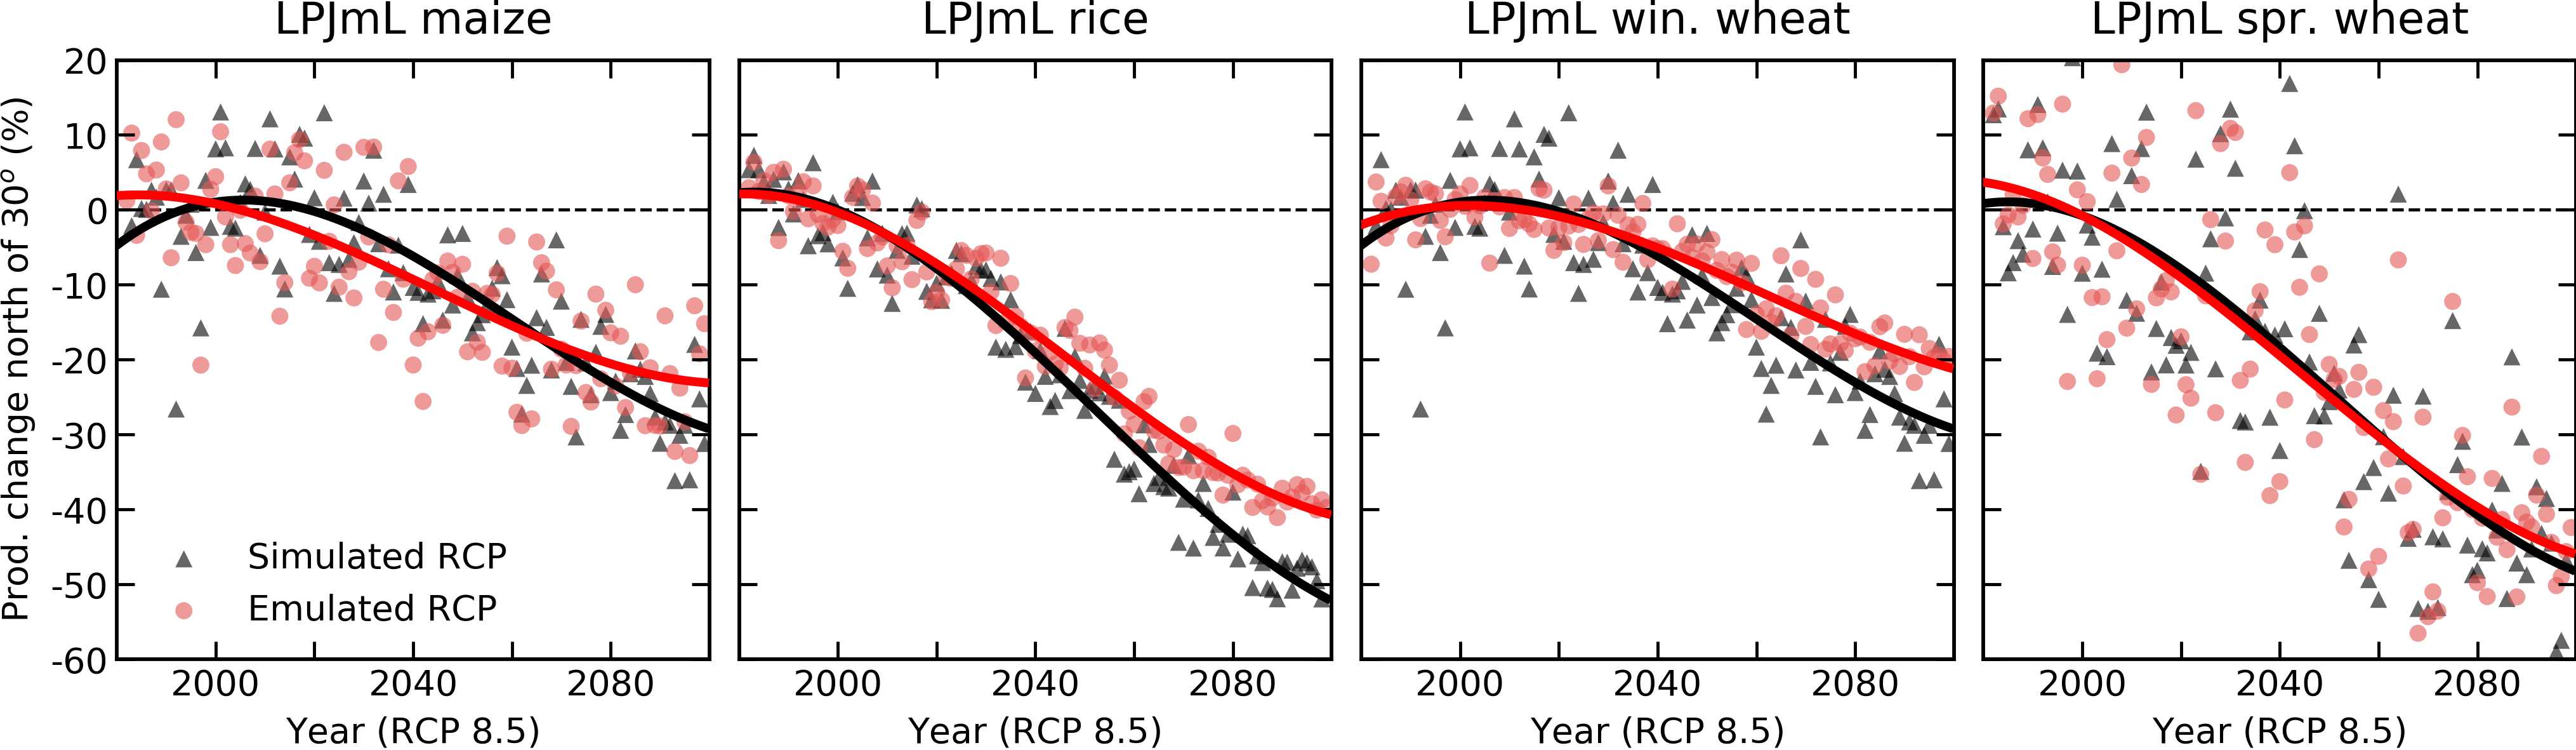
\includegraphics[width = 16.3cm]{LPJMLRCP85comp_30N.png}
  \caption{
  Illustration of the ability of the emulator to capture a more realistic future climate simulation, as in main text Figure 9 but here restricted to latitudes north of 30N.}
  \label{fig:lpjmlrcp}
\end{figure}

\clearpage
\section{Emulator products}
\begin{justify}
This section amplifies on manuscript Section 5 with additional figures analogous to manuscript Figures 10 and 11. 
\end{justify}

\vspace{0.3in}

\begin{figure}[h!]
  \centering
  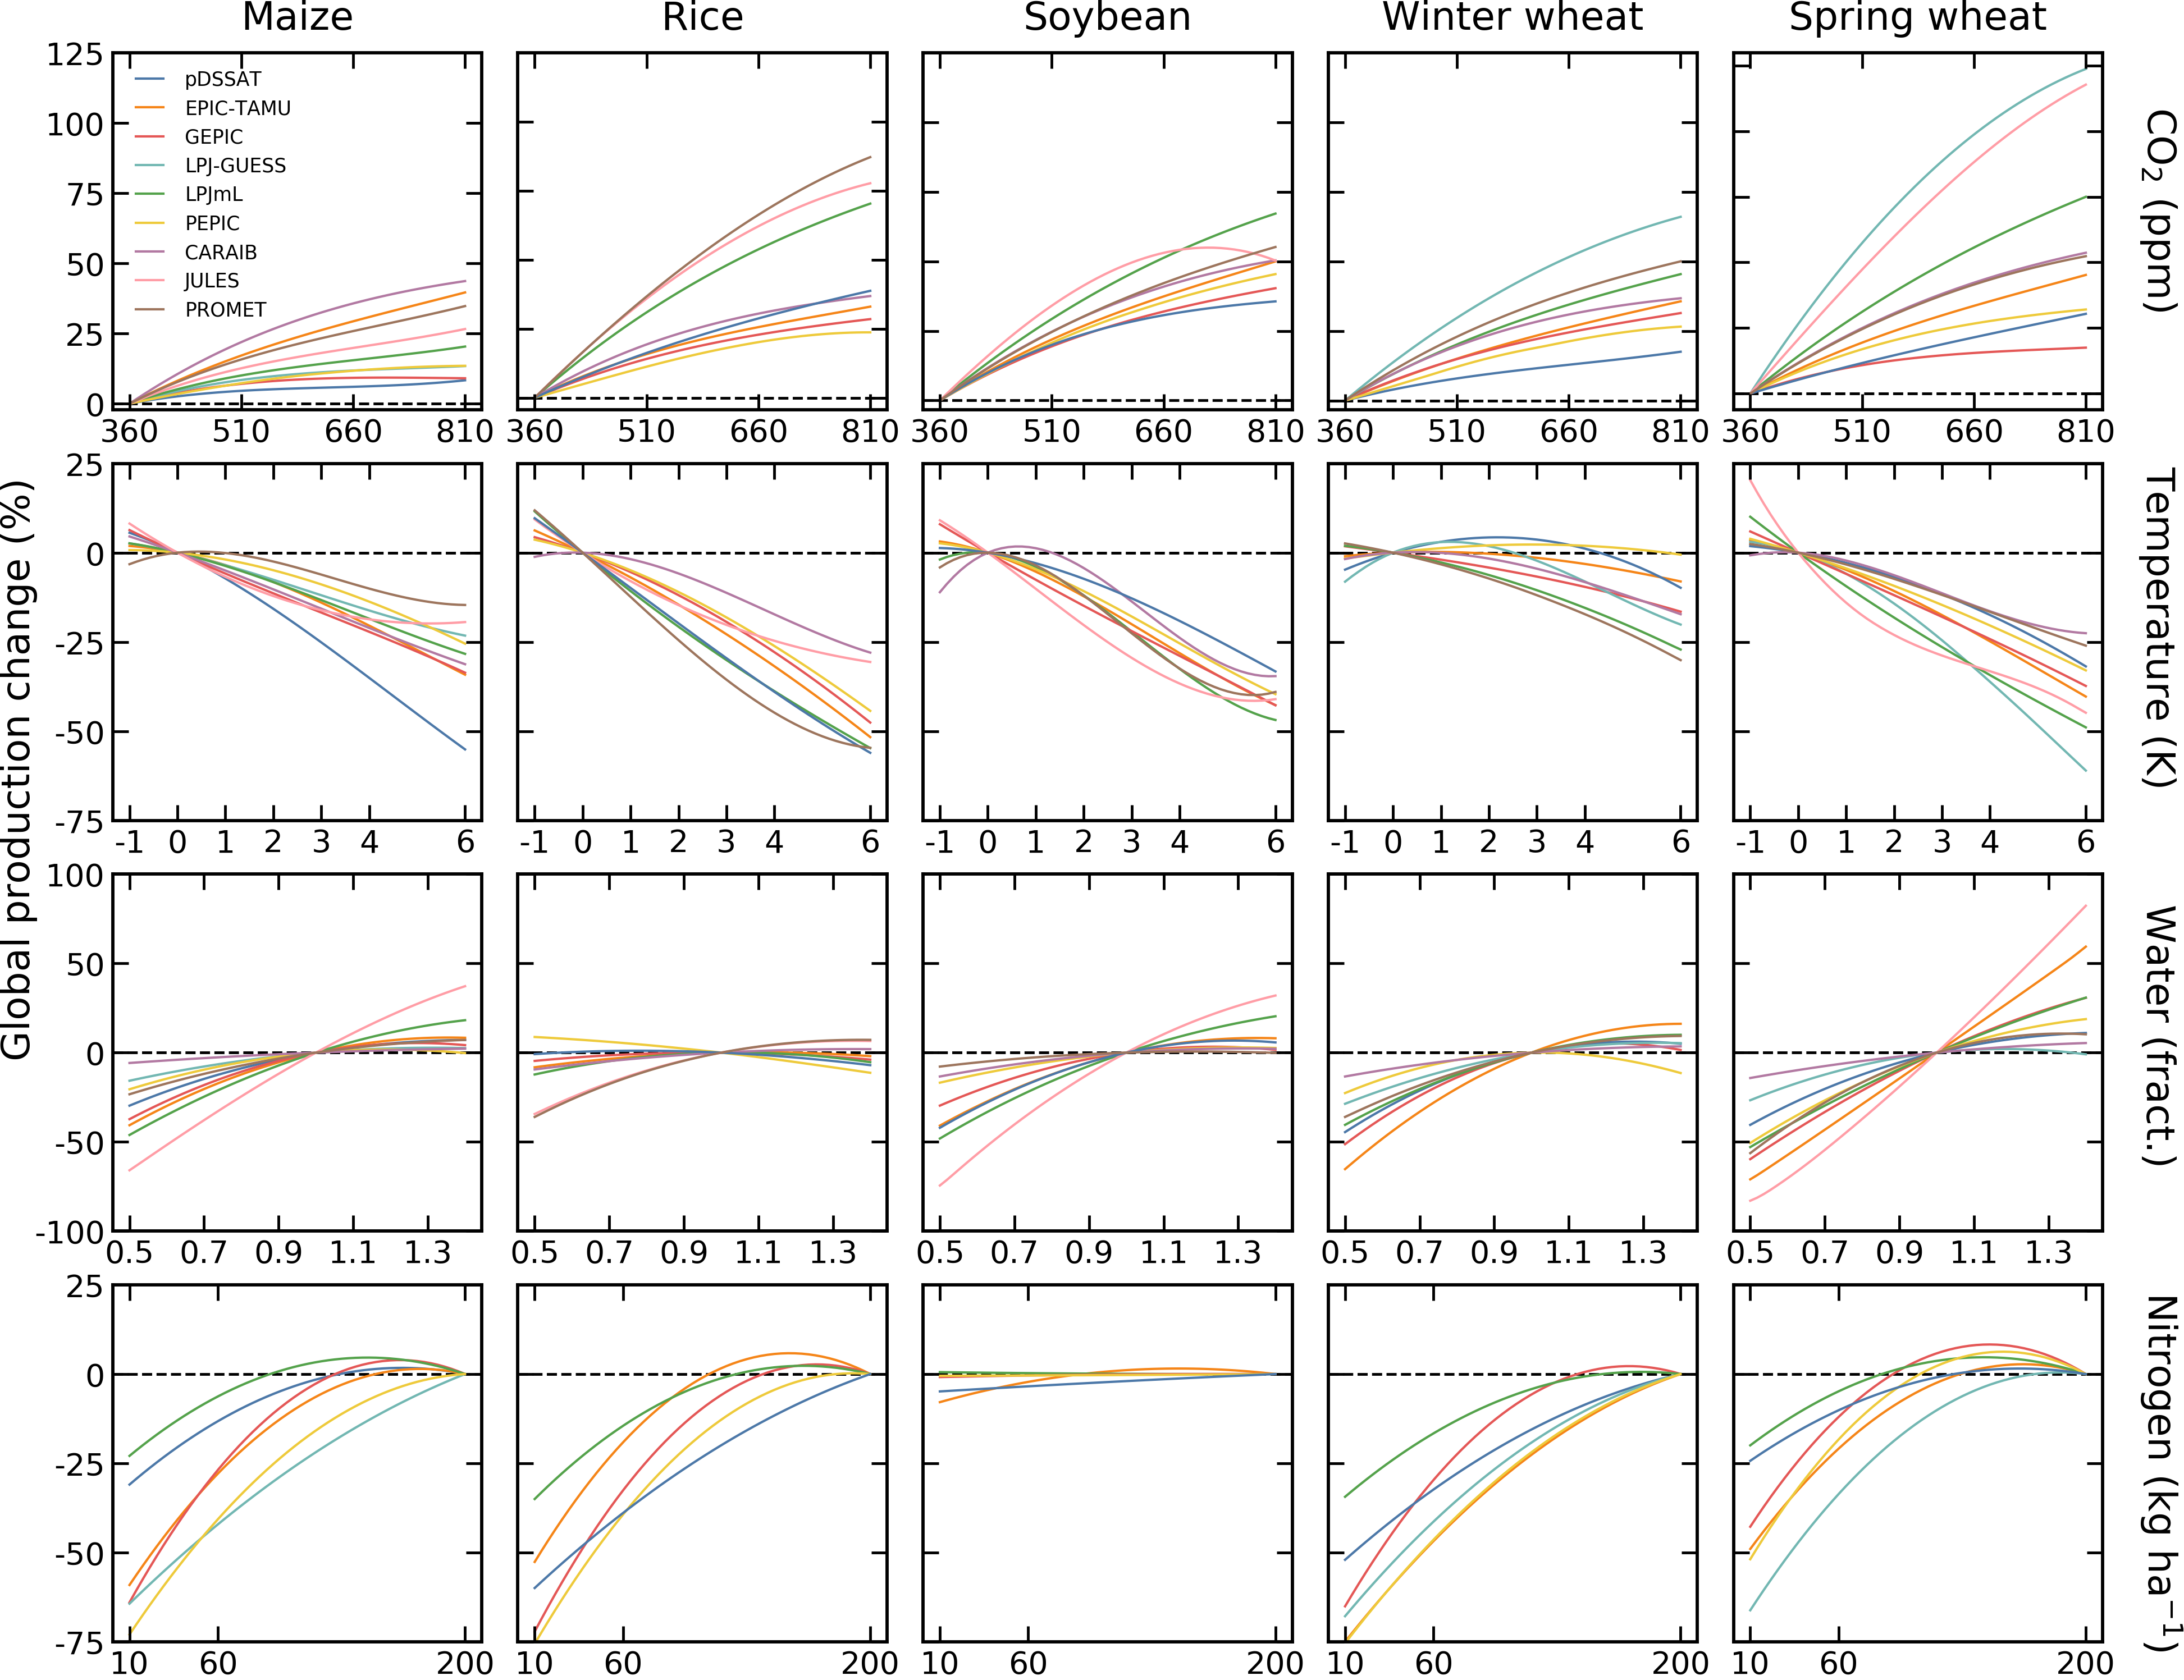
\includegraphics[width = 16.3cm]{em_CTWN_all_crops_color.png}
  \caption{
	  As in main text Figure 10 except now each model is shown in color. Not all models simulate every crop (JULES does not simulate winter wheat, and LPJ-GUESS does not simulate rice or soy) and three do not simulate the N response (CARAIB, JULES, and PROMET). For crops simulated, JULES and LPJ-GUES are often the outliers in strong CO$_2$ responses. LPJmL has the weakest N response for all crops, and pDSSAT has the strongest T response for maize.  
  }
  \label{fig:all_dims}
\end{figure}

\begin{figure}[h!]
  \centering
  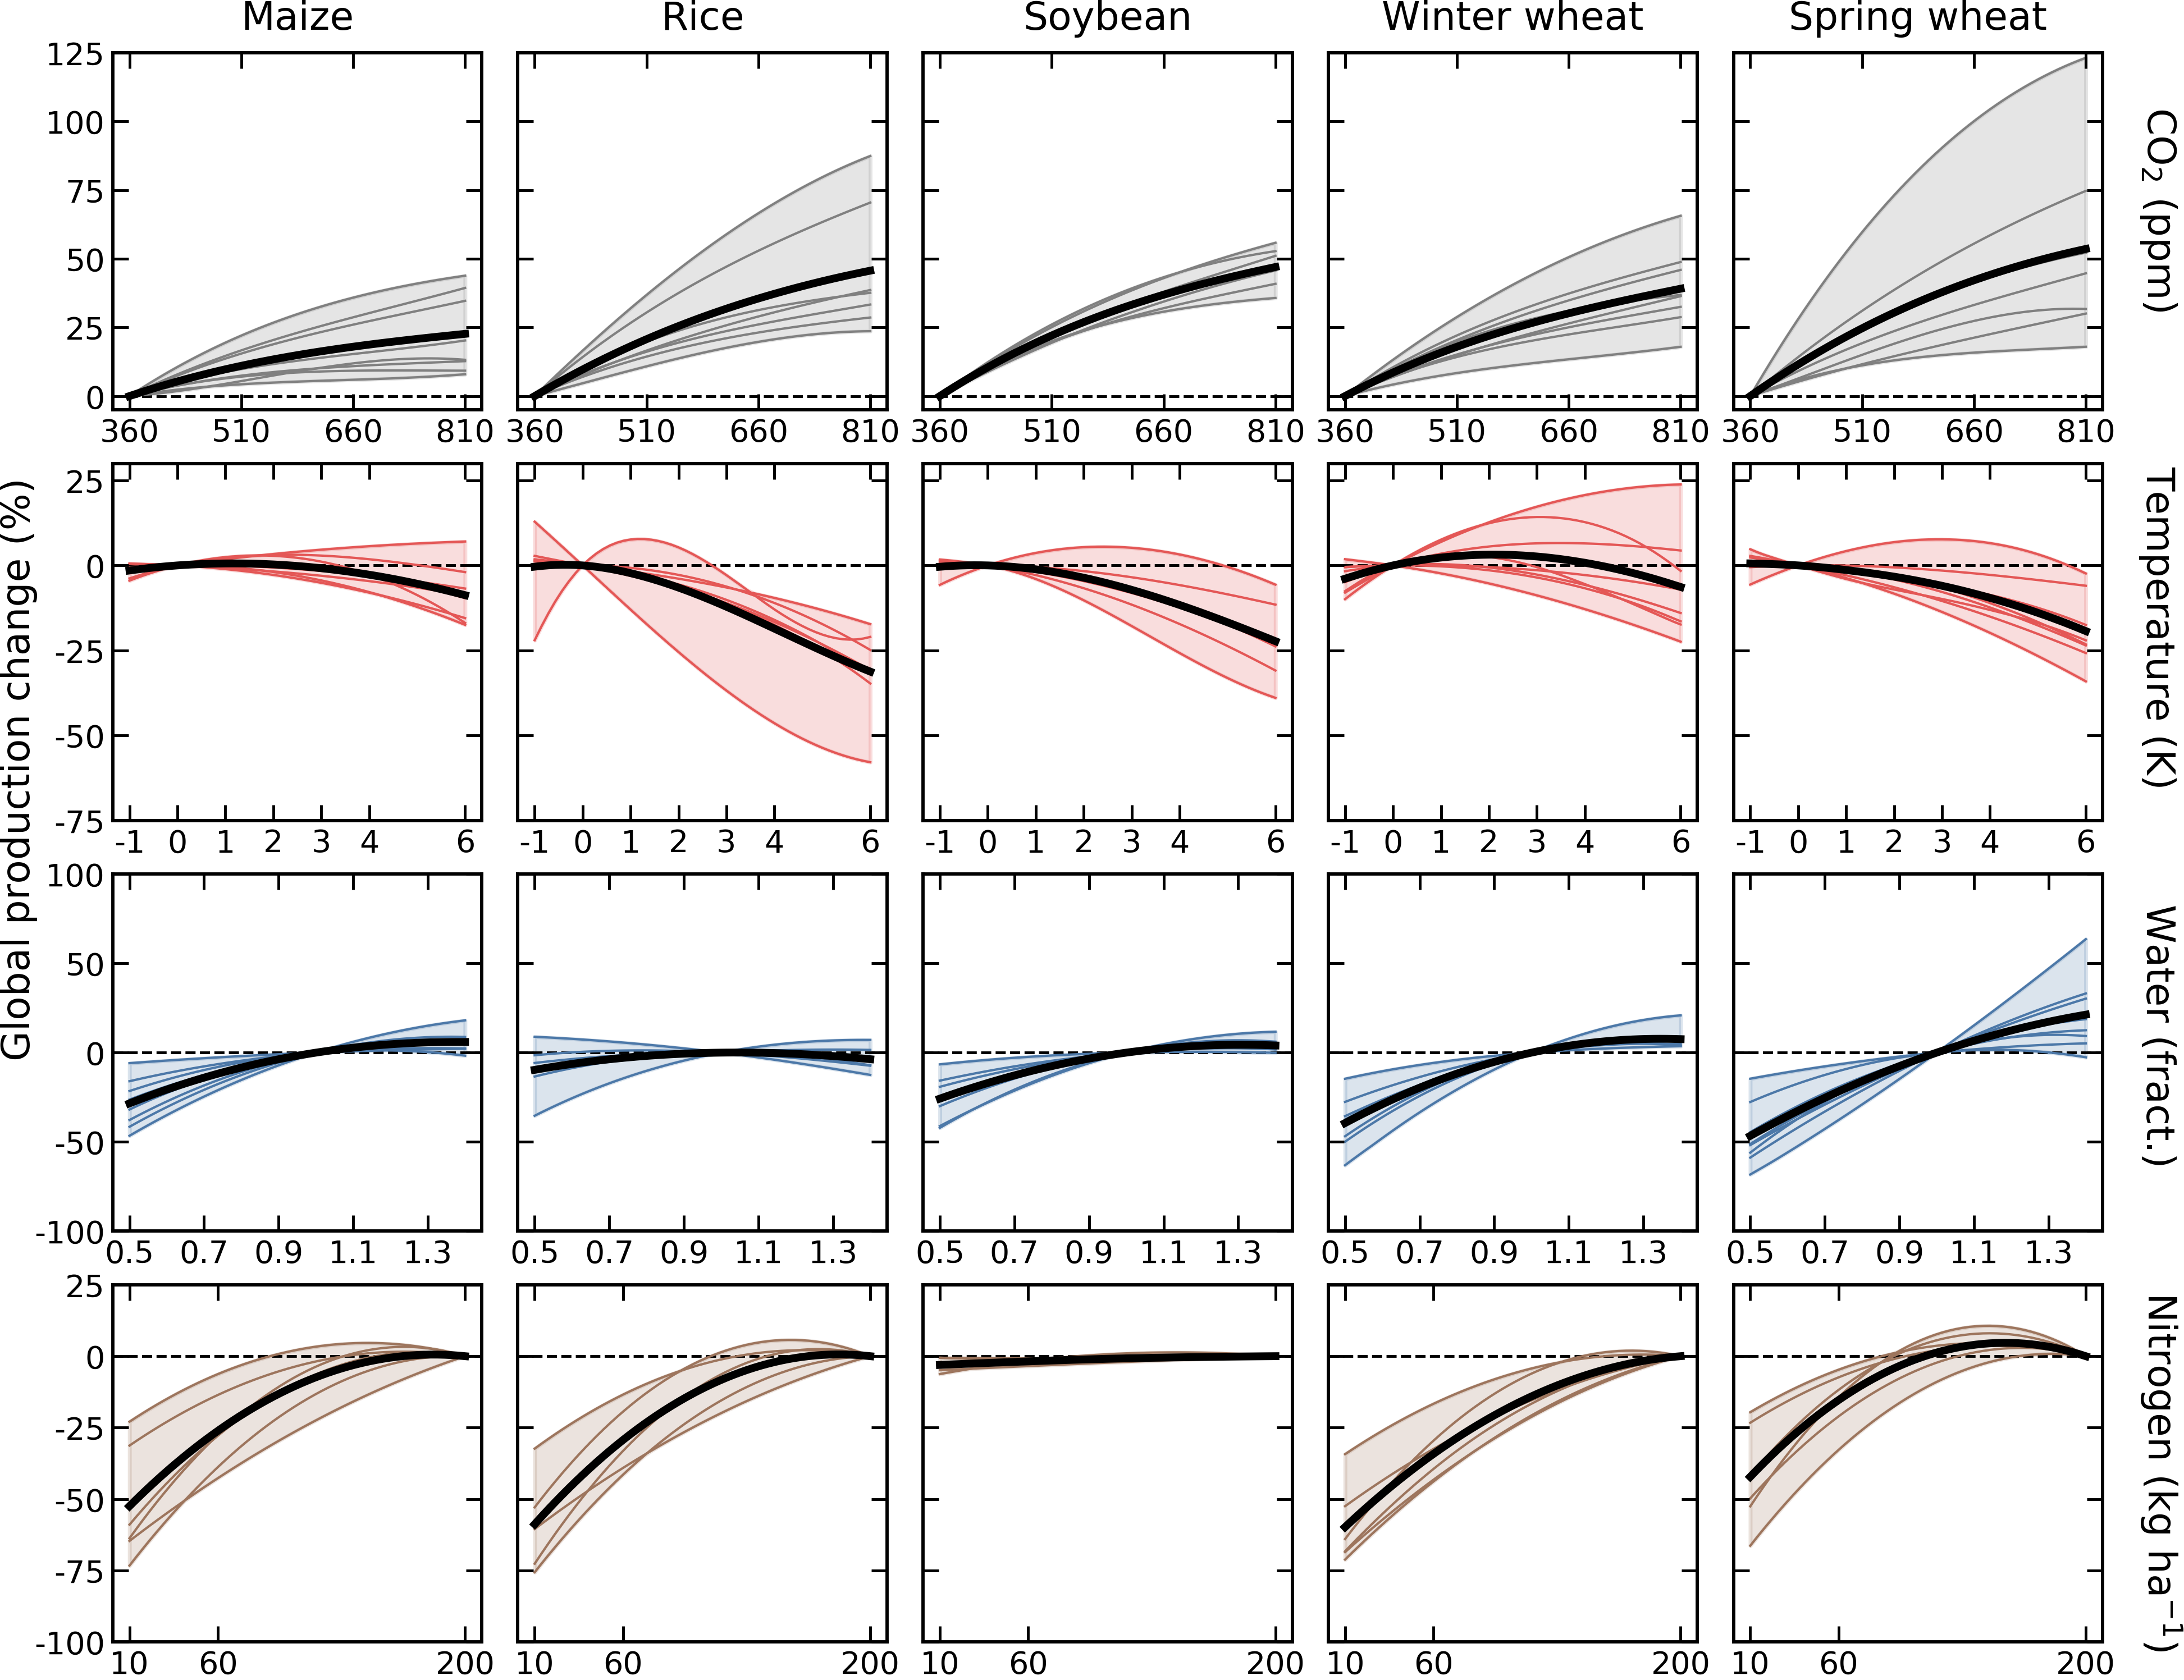
\includegraphics[width = 16.3cm]{em_CTWN_all_crops_A1.png}
  \caption{
  Emulated damage functions for rainfed crops for A1 (growing season adaptation) simulations, with conventions as in main text Figure 10 showing A0.  Temperature responses are generally flatter than for A0 simulations, but responses to other factors are similar.  Note that JULES does not provide A1 simulations. 
  }
  \label{fig:all_dims}
\end{figure}

\clearpage

\begin{figure}[h!]
  \centering
  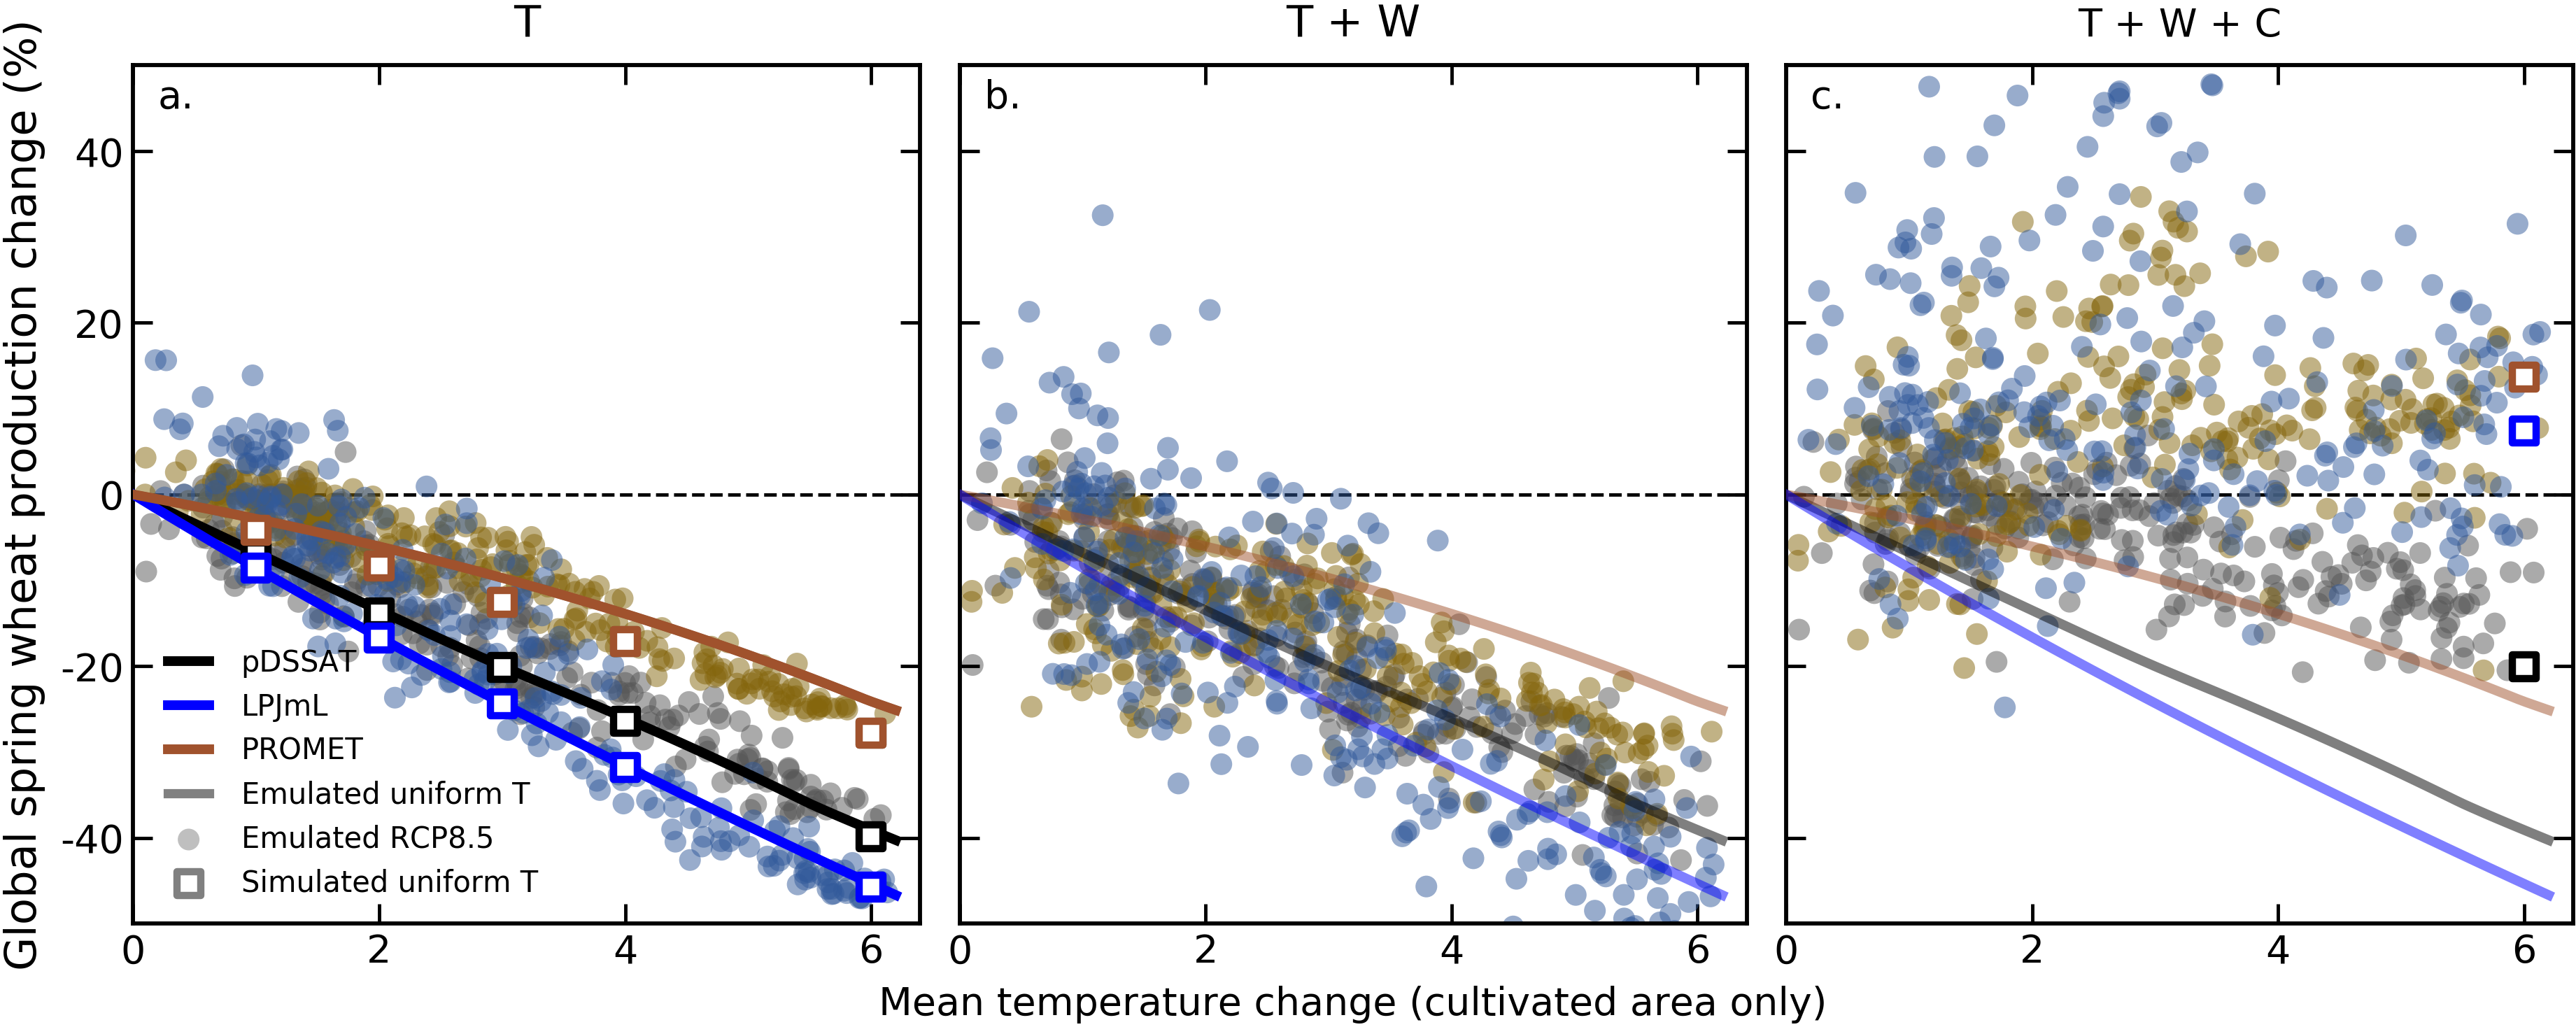
\includegraphics[width = 16.3cm]{LPJmL_pDSSAT_PROMET_RCP85_all_cases_spring_wheat.png}
  \caption{
	  Illustration of the factors affecting yields in more realistic climate scenarios for rainfed and irrigated (current mix) spring wheat. Conventions as in  main text Figure 11. Large emulator errors in PROMET spring wheat temperature response (panel \textbf{a}, compare open squares to line) are driven by Southern China, where discontinuities in yield responses make emulation problematic. (See Supplemental Material Section S11).
	  }
\end{figure}

\begin{figure}[h!]
  \centering
  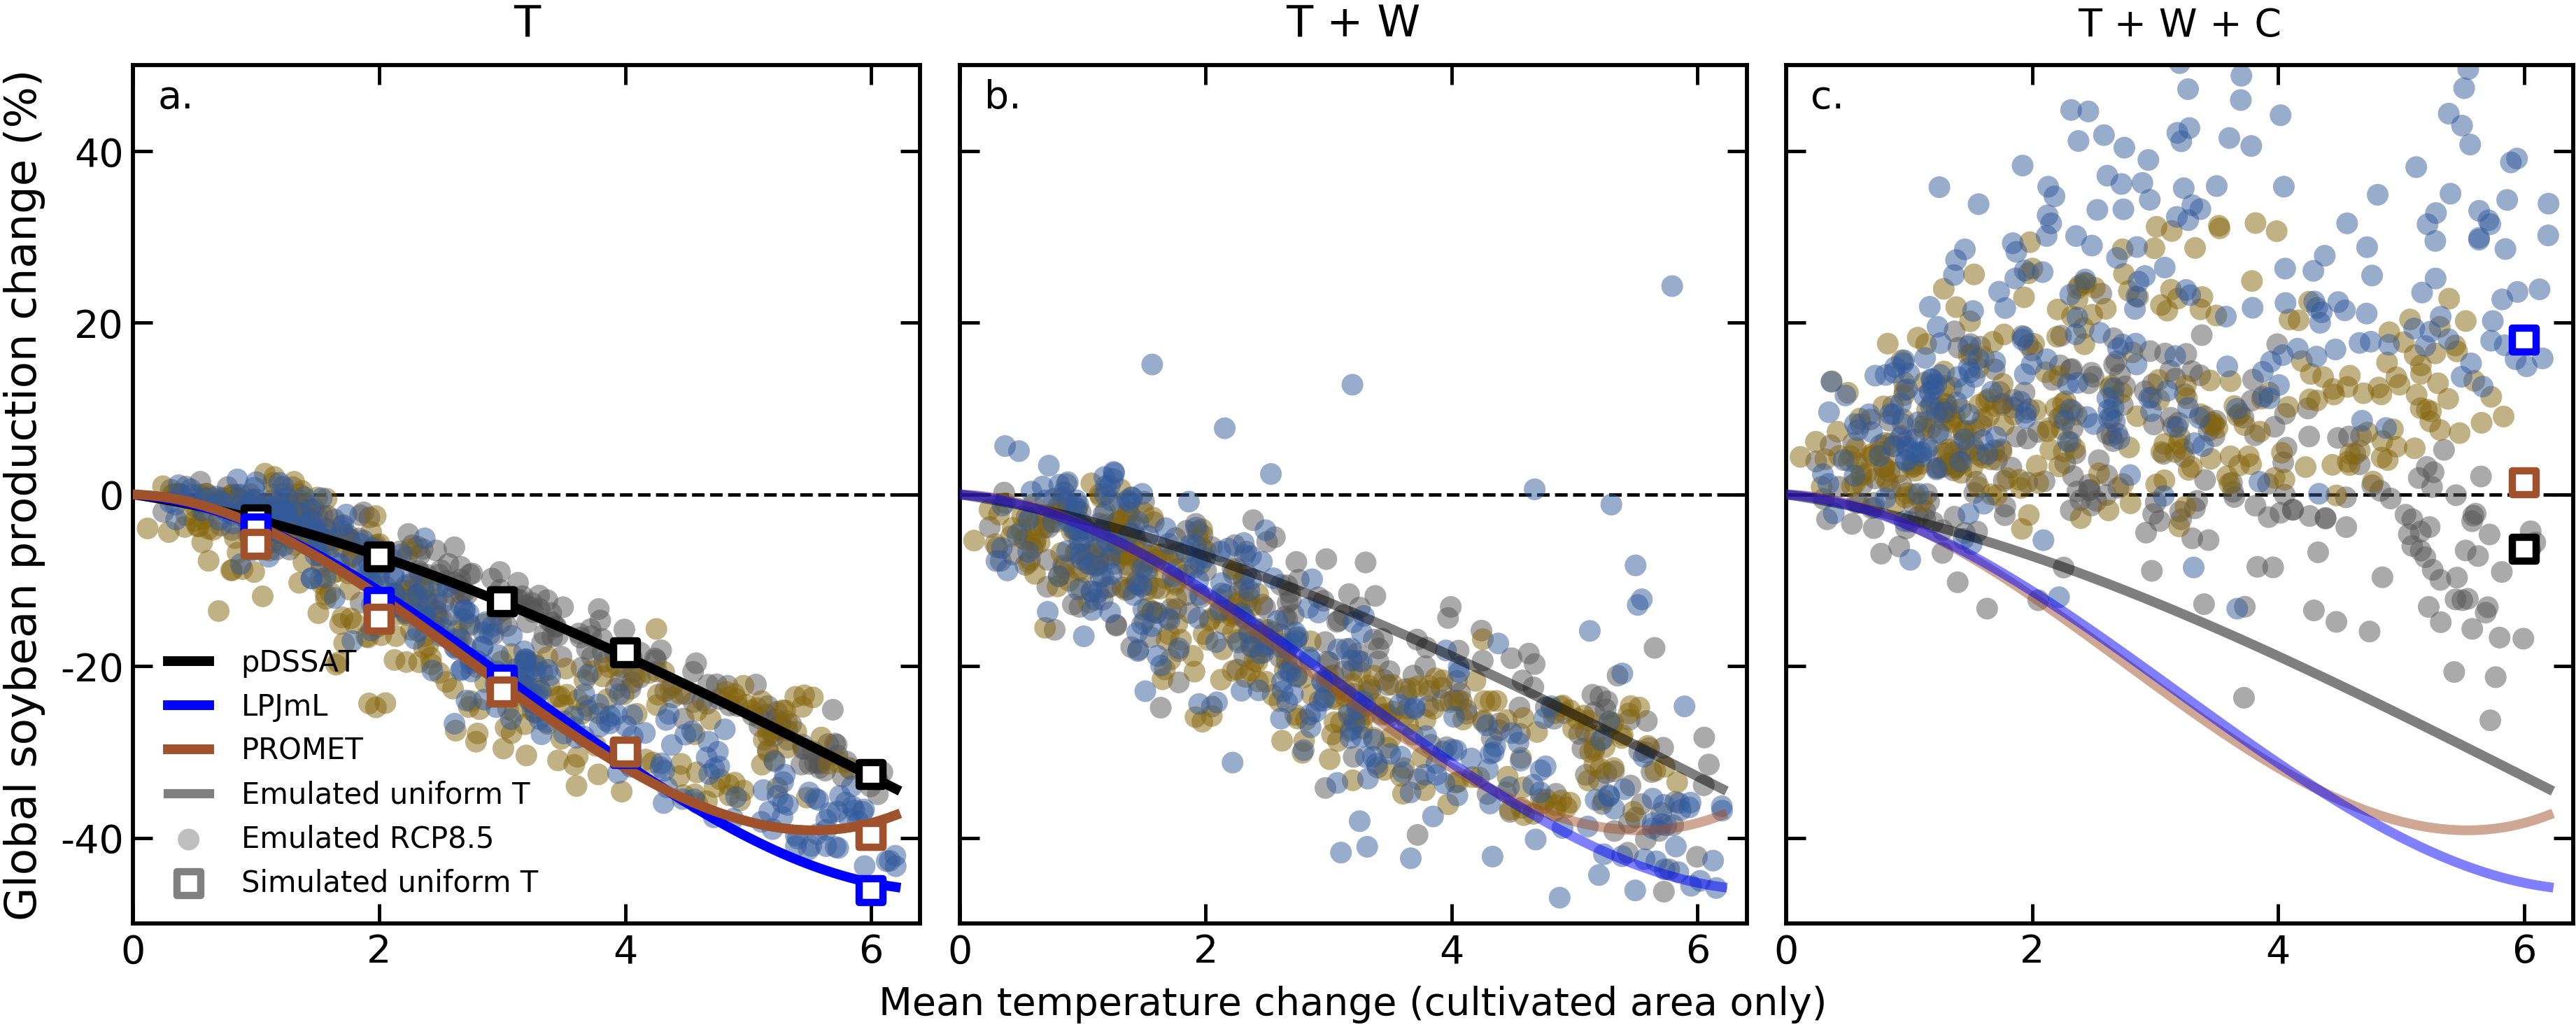
\includegraphics[width = 16.3cm]{LPJmL_pDSSAT_PROMET_RCP85_all_cases_soy.png}
  \caption{
	  Illustration of the factors affecting yields in more realistic climate scenarios for rainfed and irrigated (current mix) soy. Conventions as in main text Figure 11. The split in PROMET soybean temperature response (panel \textbf{a}, note distinct groups of points) results from the model's sensitivity to differences in spatial patterns of temperature change across climate models. 
  }
\end{figure}

\clearpage
\section{Reduced specification (23-term) emulator examples}
\smallskip
\begin{justify}
In this section we present analogous figures to those in the main text for the reduced-form (23-term) emulator. 
Issues with the reduced-form model are most prominent in PROMET for rice and soy, and JULES soy and spring wheat. 
We identify several potential factors that may in some way contribute to these models showing qualitatively different responses that require additional terms for emulation.
	\begin{itemize}
		\item PROMET and JULES do not allow nitrogen variation. (However, CARAIB also cannot vary N and is readily emulatable with the 23-term specification.) 
		\item Both JULES and PROMET models are land system process models, originally developed with a broad focus, which have been adapted for managed vegetation (agriculture) only recently (2015). (CARAIB, by contrast, was originally developed as a vegetation model in the early 90's and has a longer history of agricultural focus.)
		\item Both PROMET and JULES have anomalously strong responses to individual factors in those crops problematic to emulate. PROMET is the most sensitive model of all the models for rice in C, T, and W, and JULES for soybeans in C, T, and W. For spring wheat, JULES is a high outlier in C, the most sensitive model in W and T, and shows an extra inflection point in the global temperature response not seen in any of the other models.
		\item PROMET is the quantitatively lowest-performing model for soybeans when compared to the historical FAO data for the top 10 producing countries. 
		\end{itemize}
\end{justify}
%\smallskip
%\begin{justify}
%CARAIB on the other hand (the other model that does not simulate different levels of nitrogen), was originally developed as a vegetation model in the early 90's and has a longer history of agricultural focus. It is the least sensitive model in T for rice and spring wheat, and is nearest to the ensemble mean in maize and winter wheat. 
%In W, it is the least sensitive model for maize, and the wheats, the second least sensitive model for soybeans, and nearest to the ensemble mean for rice. 
%For C, it is the nearest to the ensemble mean for the wheats and soy and unremarkable for rice. 
%However, CARAIB is the most sensitive model for maize in the C dimension (though this is relatively less sensitive than most other responses for other models the other crops).
%\end{justify}

% 15.5
\vspace{-0.1in}
\begin{figure}[h!]
  \centering
  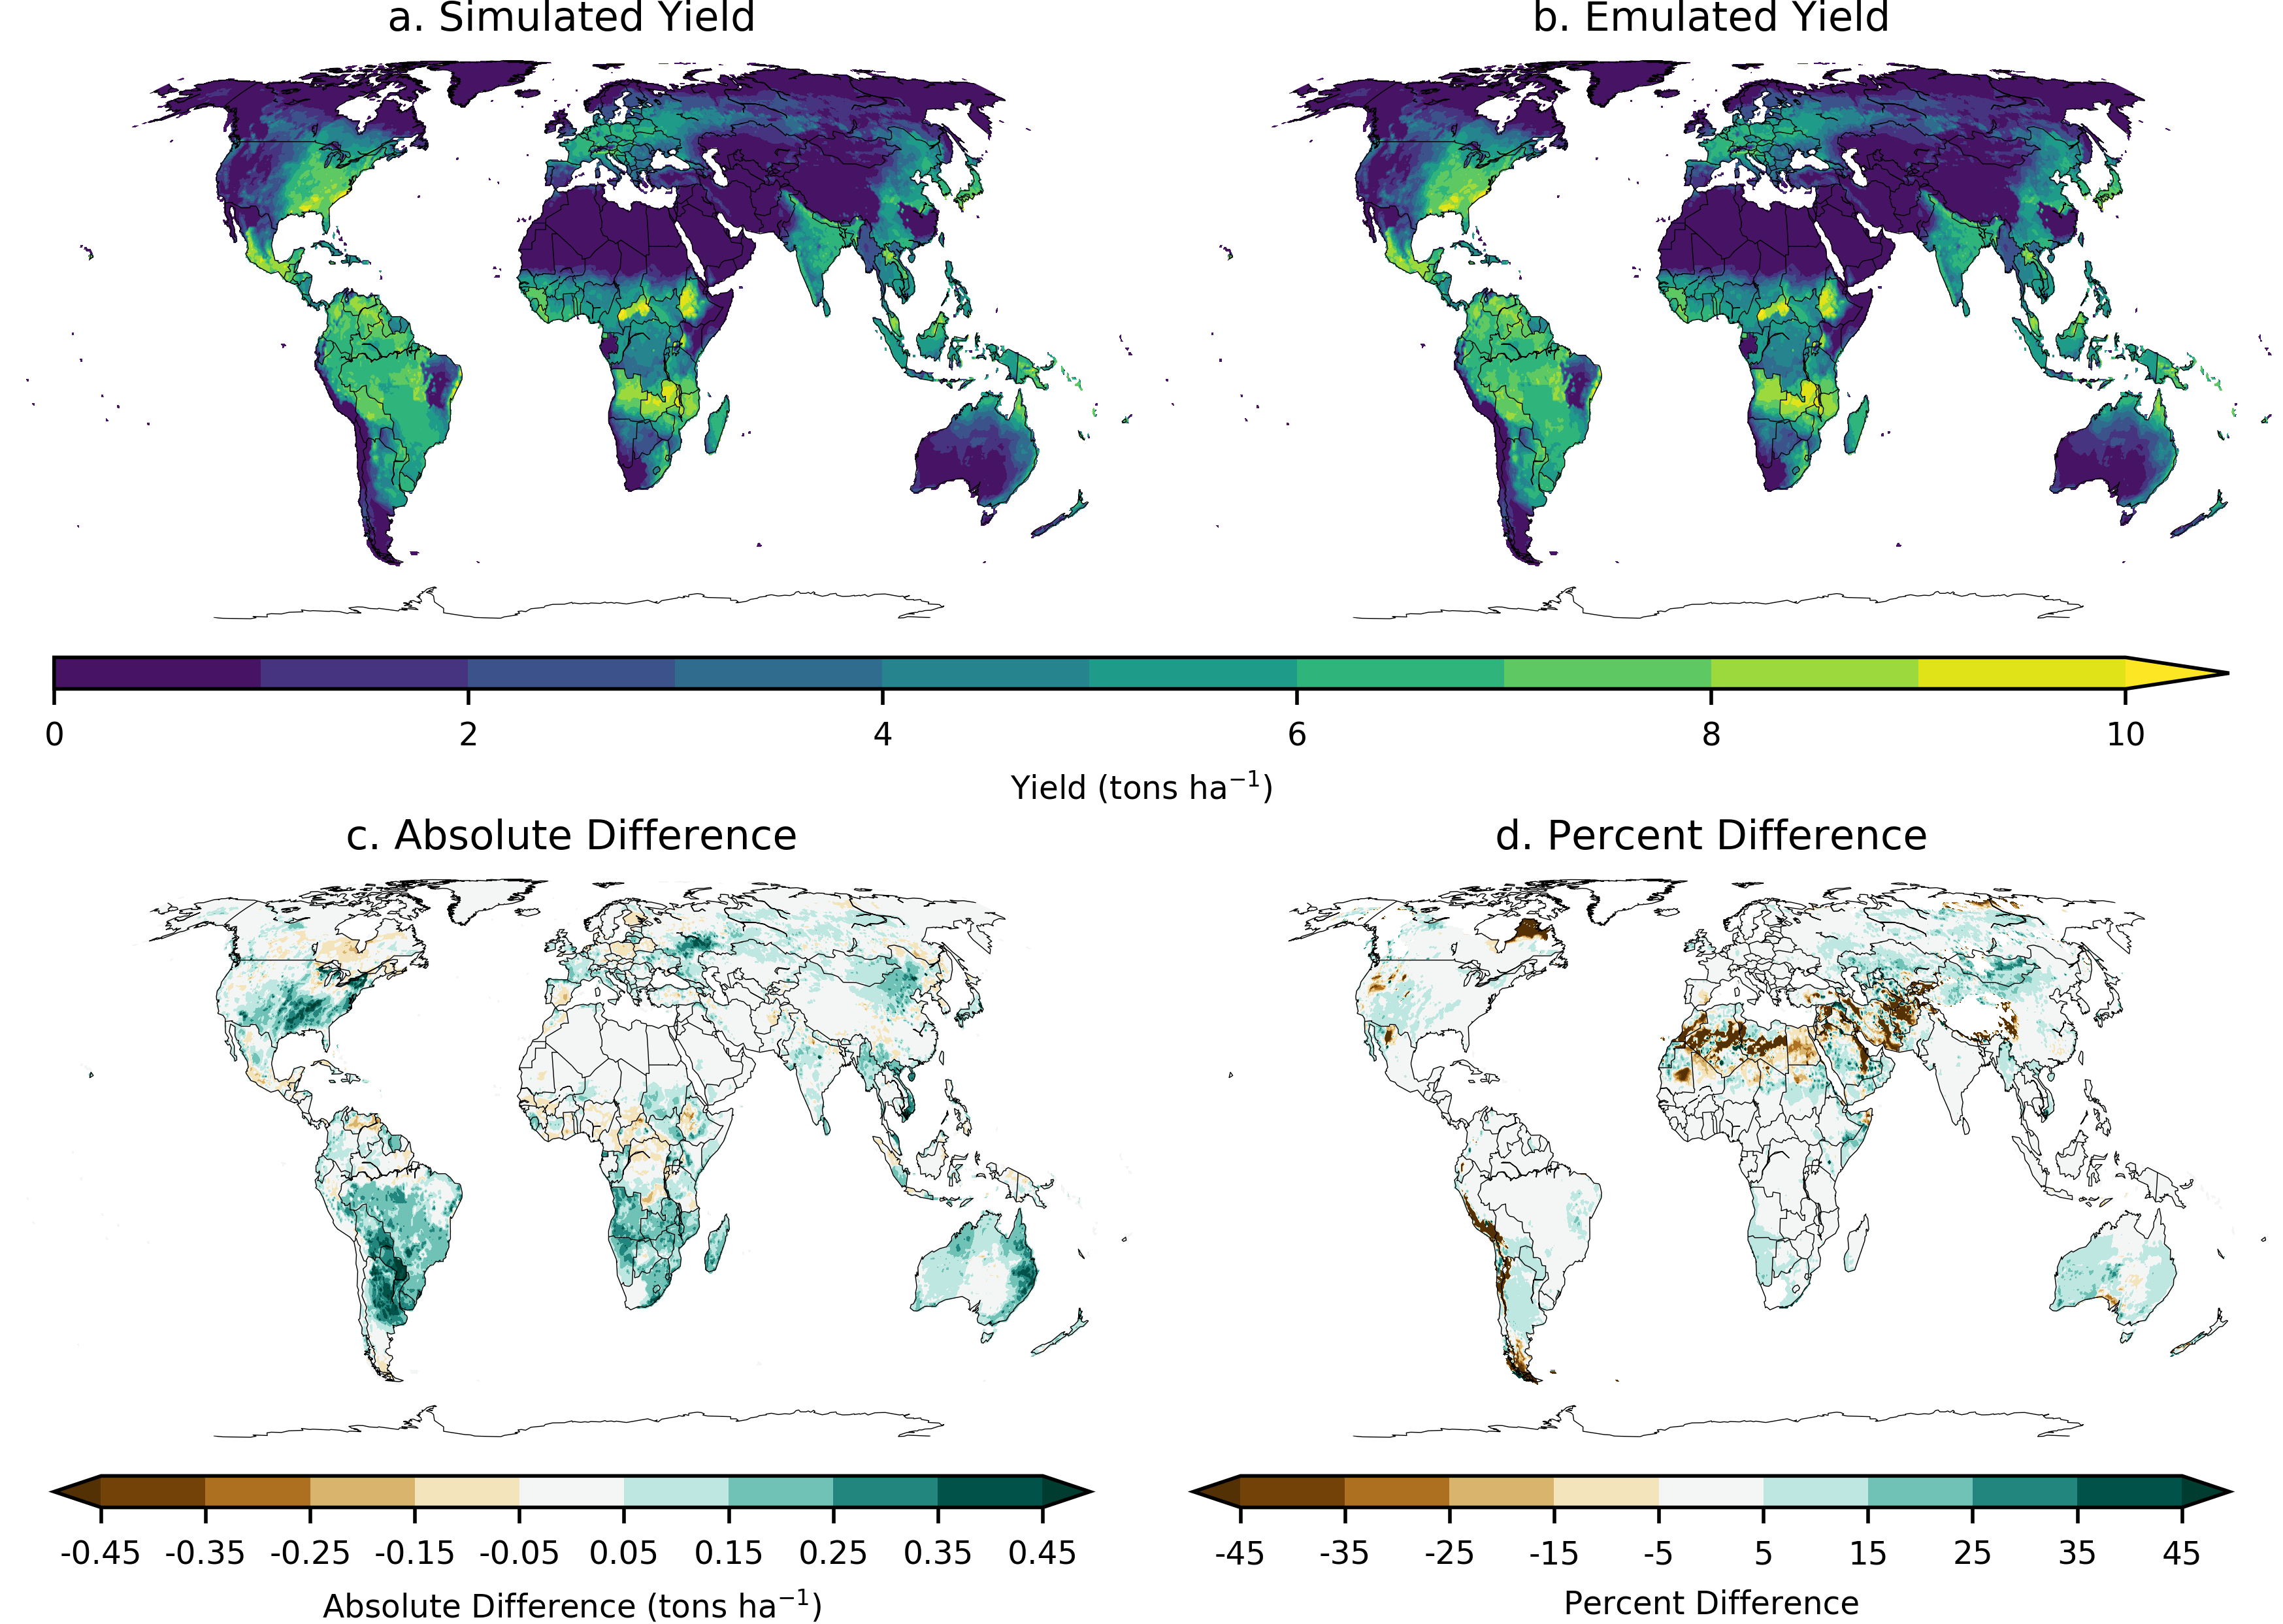
\includegraphics[width=11.cm]{reduced_lpjml_maize.png}
  \caption{As in manuscript Figure 4,  simulated (a.) and emulated (b.) yield under historical conditions for rainfed LPJmL maize, but here for the reduced (23-term) emulator specification. Emulator performance is worse primarily where crops are not currently grown.}
  \label{fig:reducedlpjml}
\end{figure}

\begin{figure}[h!]
  \centering
  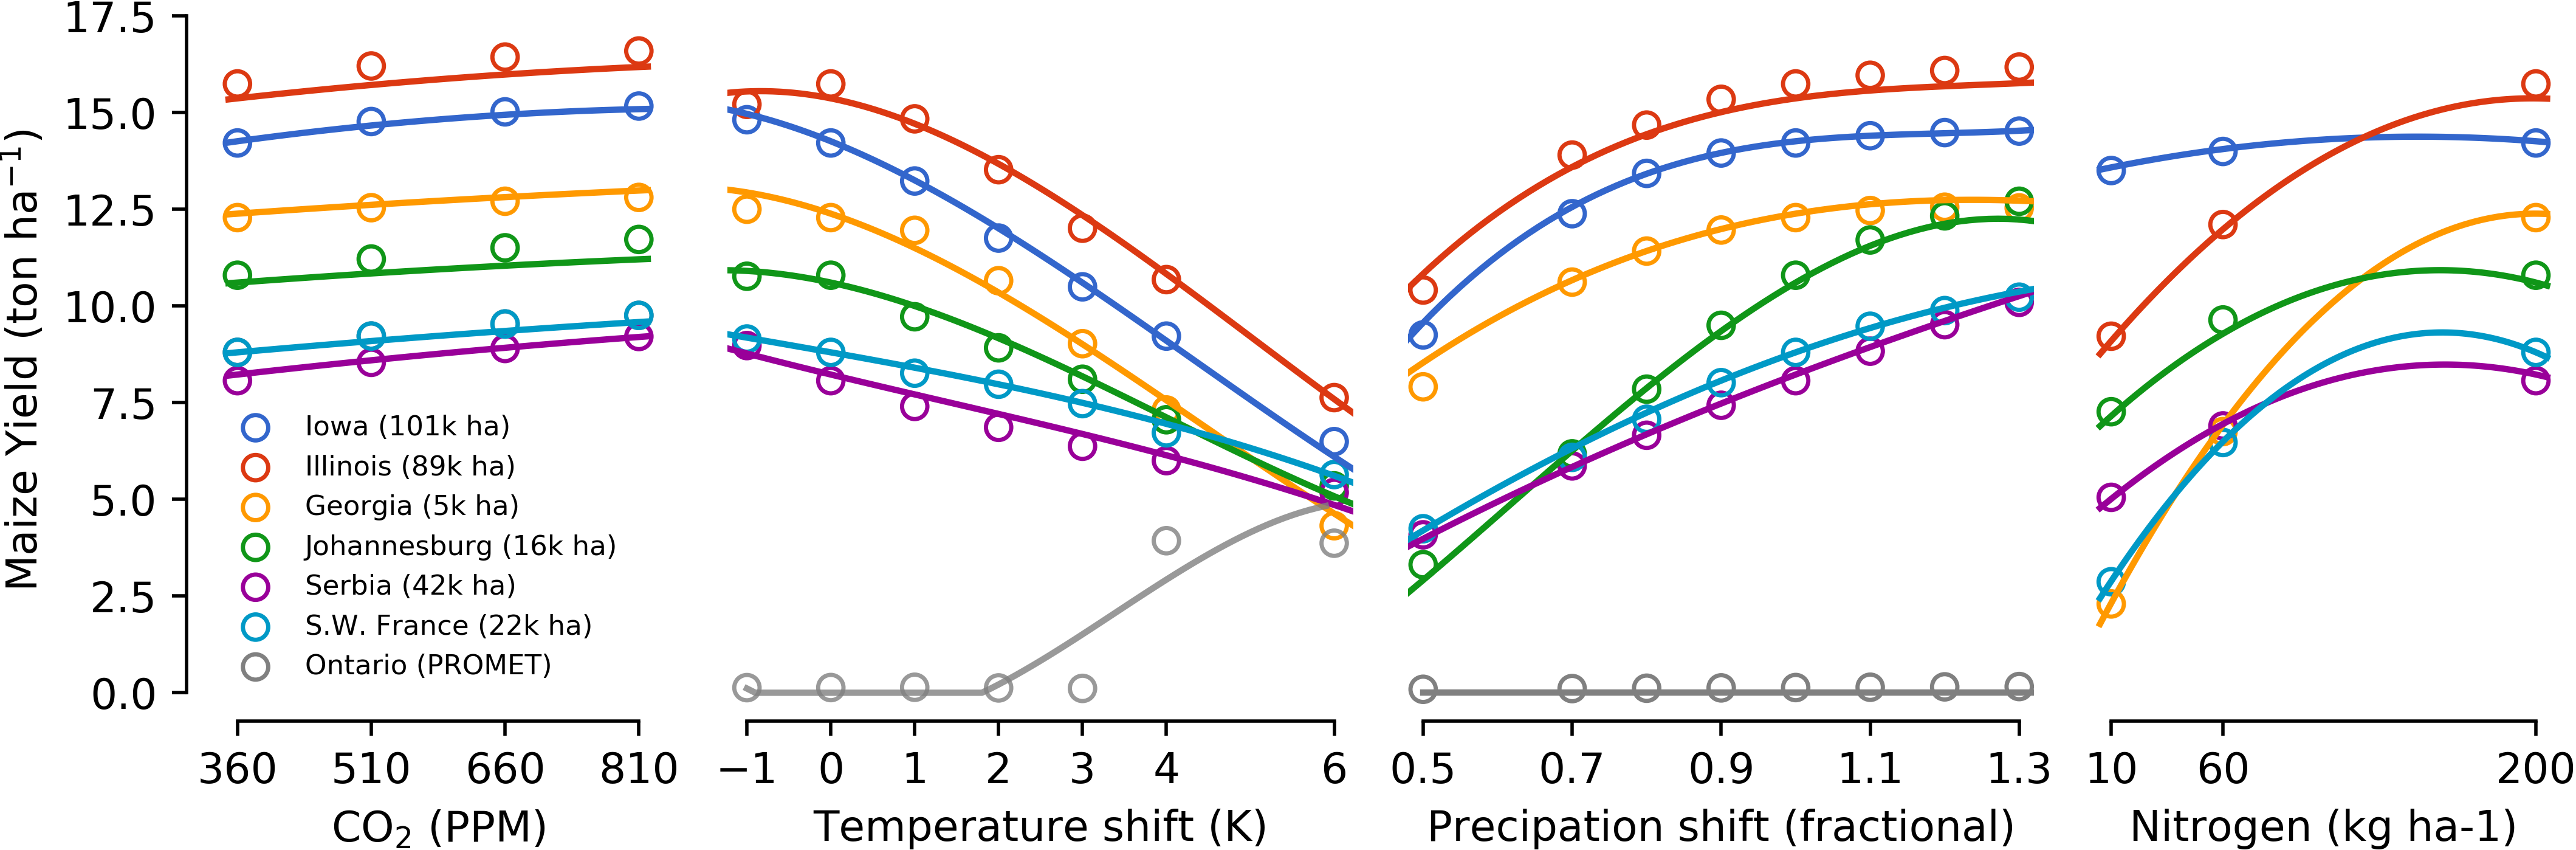
\includegraphics[width=15.5cm]{reduced_regression_example_1.png}
	\caption{As in manuscript Figure 5, emulator performance in selected high-yield regions for rainfed pDSSAT maize (and one region for PROMET), but now with the reduced (23-term) emulator specification. Emulator performance is similar.}
  \label{fig:reducedareas}
\end{figure}

\begin{figure}[h!]
  \centering
  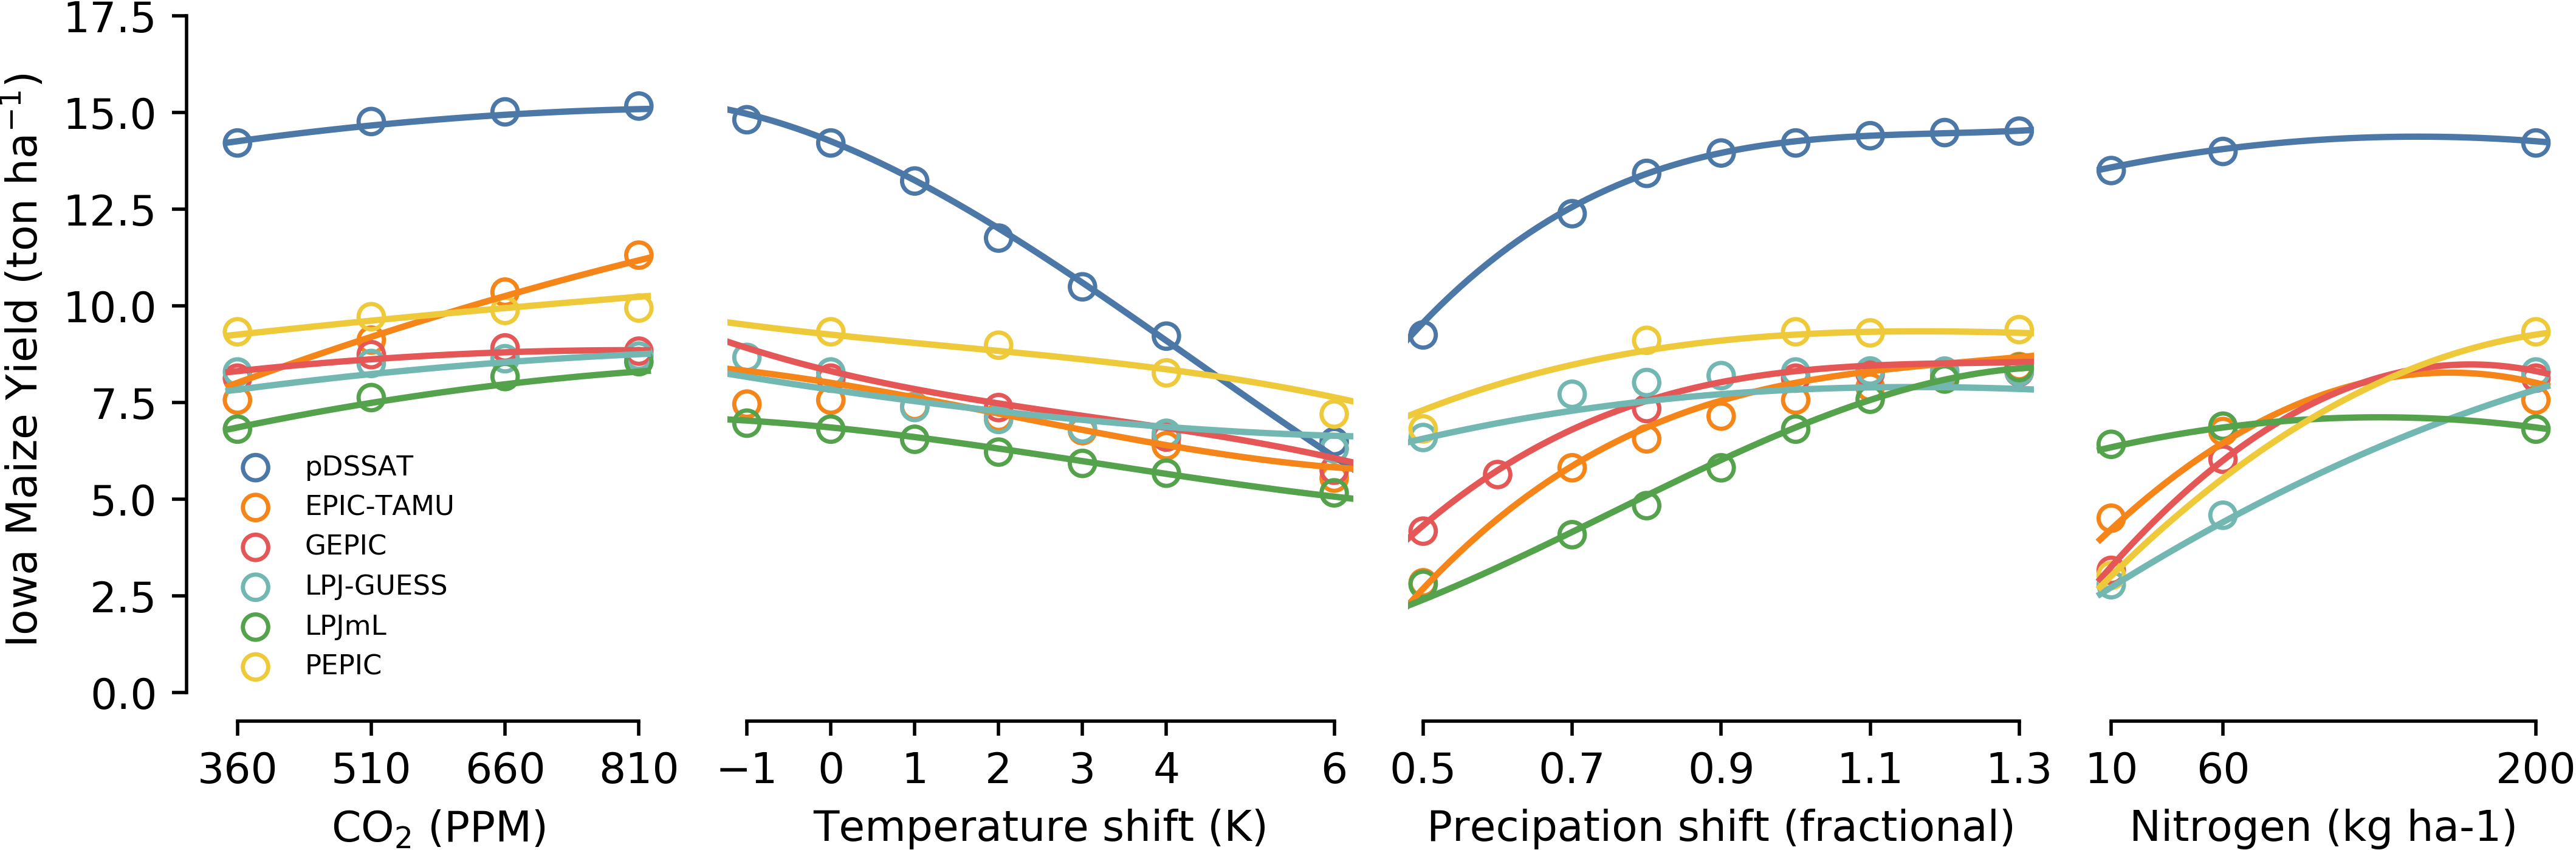
\includegraphics[width=15.5cm]{reduced_regression_example_2.png}
  \caption{As in manuscript Figure 6, emulator performance across models for rainfed maize in one grid cell in Iowa, but now with the 23-term emulator specification. Note that JULES and PROMET are not shown.}
  \label{fig:reducedmodels}
\end{figure}

\begin{figure}[h!]
  \centering
  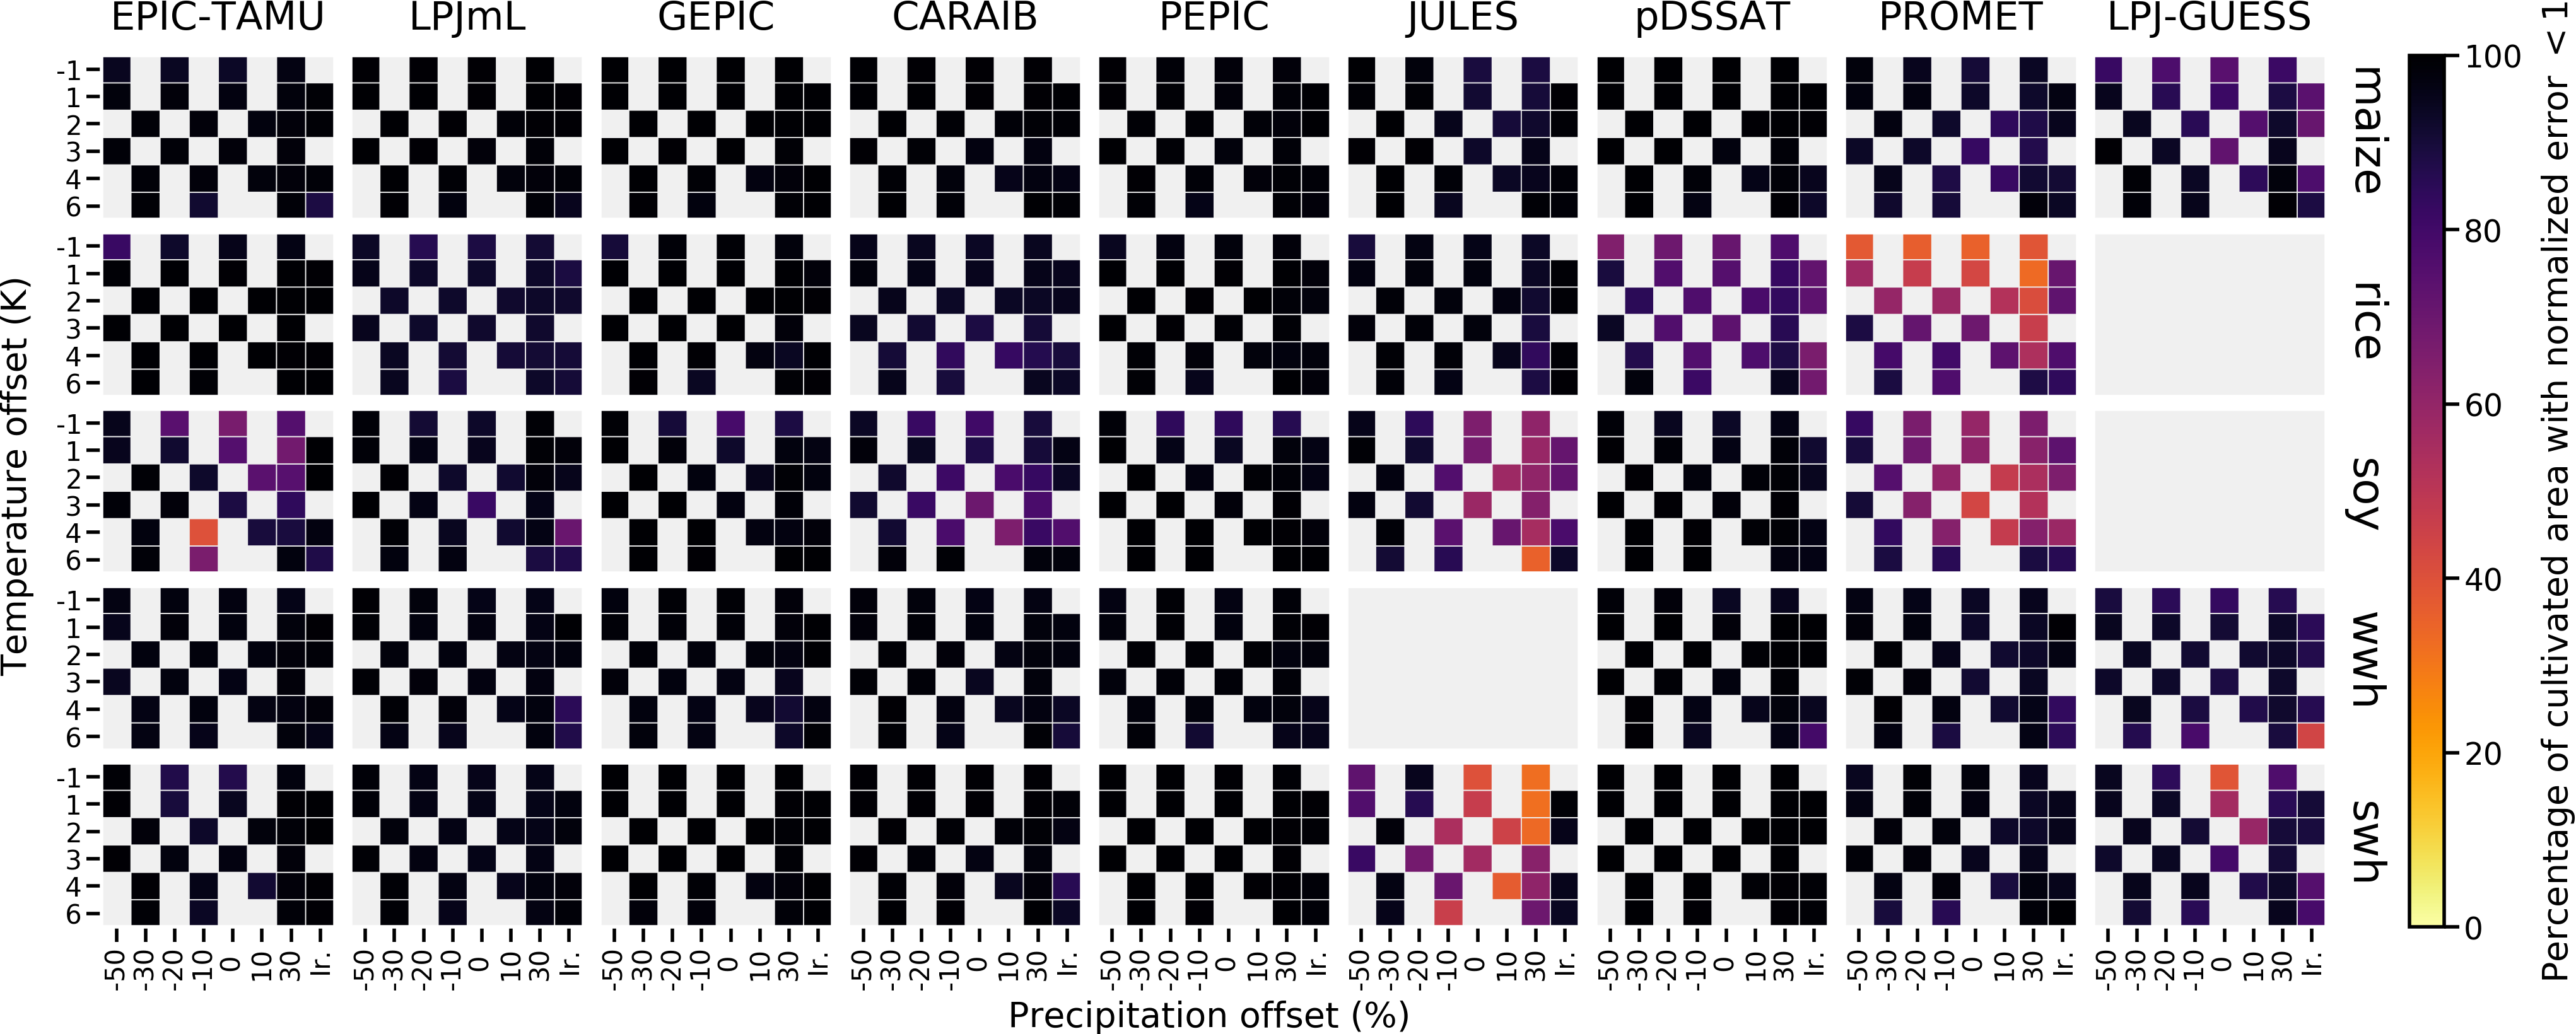
\includegraphics[width=15.5cm]{reduced_error_grid.png}
  \caption{
  As in manuscript Figure 7, normalized error of all 9 models emulated on currently cultivated land, over all crops and all sampled T and W inputs, with CO$_2$ and nitrogen held fixed at baseline values, now with the reduced (23-term) emulator specification. Degradation of performance is most evident in JULES soy and spring wheat and PROMET rice and soy.
  }
  \label{fig:reducedgrid}
\end{figure}

\begin{figure}[h!]
  \centering
  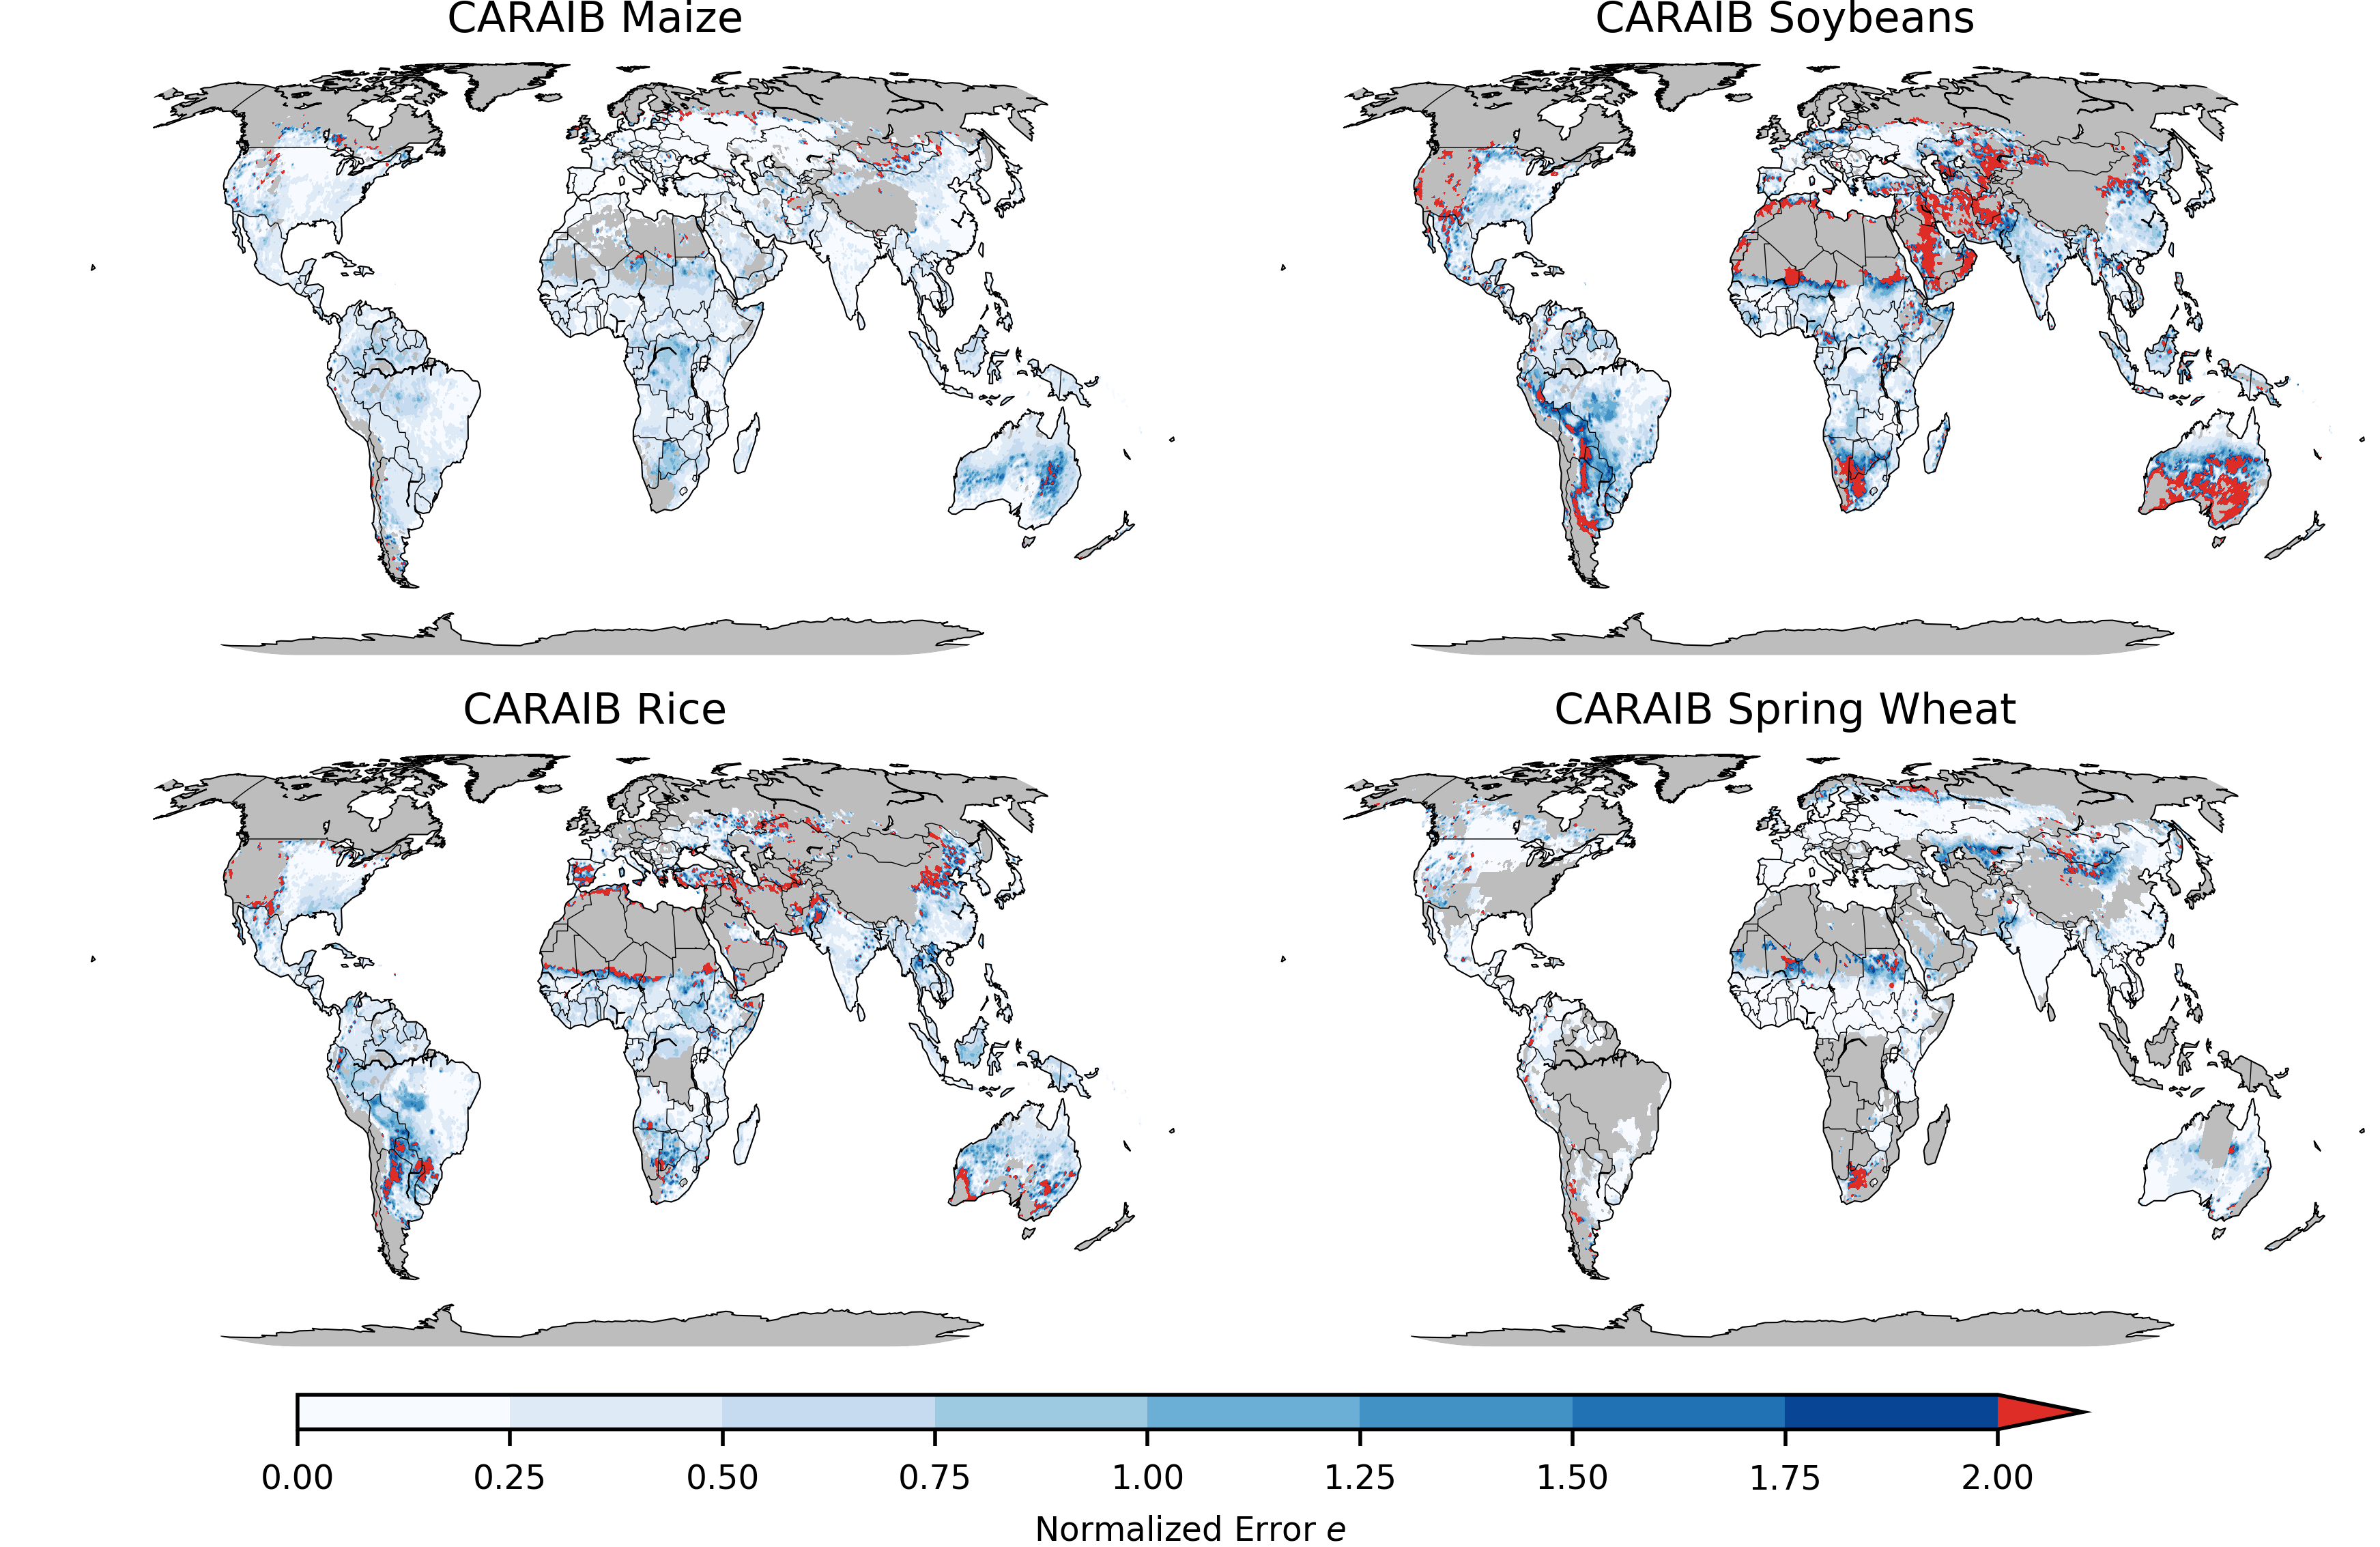
\includegraphics[width=15.5cm]{reduced_CARAIB_spatial_error.png}
  \caption{
  As in manuscript Figure 8, normalized error for rainfed crops in CARAIB for the T+4 scenario, but here with the reduced (23-term) emulator specification. Degradation of performance is most evident in marginal lands where crops are not currently grown.
  }
  \label{fig:reducedcaraib}
\end{figure}

\begin{figure}[h!]
  \centering
  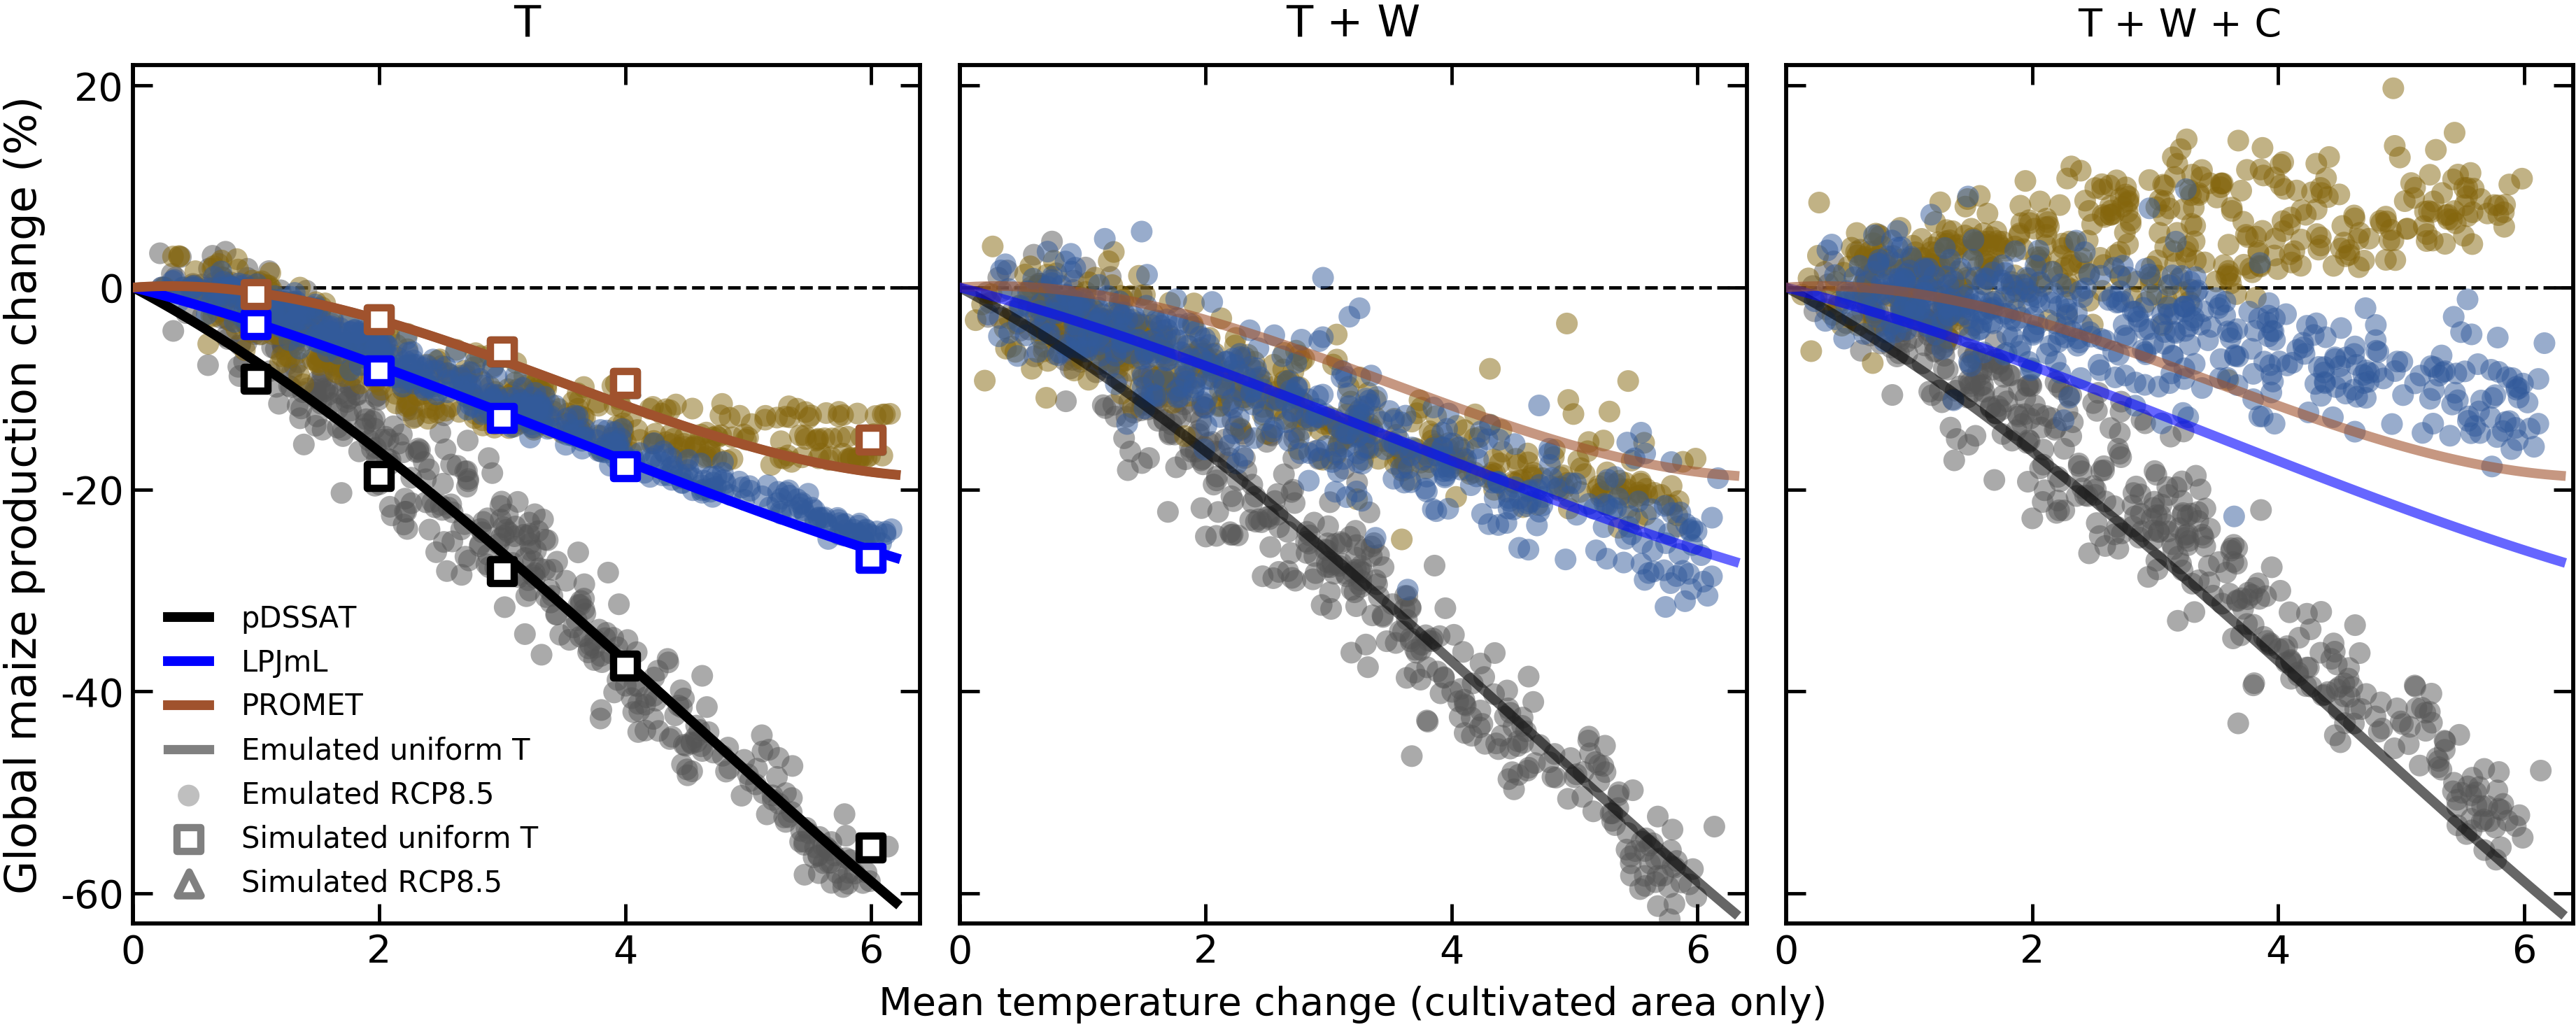
\includegraphics[width = 16.3cm]{reduced_global_em_maize.png}
  \caption{
  As in manuscript Figure 11, rainfed maize on currently cultivated land, but here with the reduced (23-term) emulator specification. Note that strong C response for PROMET is different here than with the full-form emulator, because higher order C ($C^{3}$, $C^{2} * T$ ...) interaction terms are needed for accurate emulation. 
  }
\end{figure}

\begin{figure}[h!]
  \centering
  \includegraphics[width=14cm]{JULES_soy_bad.png}
  \caption{
  Example of emulator failure, showing failure induced because of strongly interacting terms. 
  Simulated and emulated values for JULES soybeans in Southern Germany. RMSE = 41\% of baseline yield for the reduced form (23-term) emulator.
  The downturn in yields as C and W increase can only be captured by the higher order C interaction terms of the full 34-term specification. 
  }
  \label{fig:lpjmlrice}
\end{figure}

\begin{figure}[h!]
  \centering
  \includegraphics[width=14cm]{PROMET_rice_bad.png}
  \caption{
	  Example of emulator failure, showing failure induced by abrupt changes in yields. Simulated and emulated values for PROMET rice in India (Arunachal Pradesh). RMSE = 132\% of baseline yield for red (reduced fit).
  The step change in the yields around 0 K at higher water specifications cannot be captured by any third order polynomial. 
  Both 23- and 34- emulator specifications fail in this example.
  }
  \label{fig:lpjmlrice}
\end{figure}

%%%%%%%%%%%%%%%%%%%%%%%%%%%%%%%%%%%%%%%%%%%%%%%%%%%%%%%%%%%%%%%%%%%%%%%%%%%%%%%%%%%%%%%%%%%%%%%%%%%%%%%%%%%%%%%%
%%%%%%%%%%%%%%%%%%%%%%%%%%%%%%%%%%%%%%%%%%%%%%%%%%%%%%%%%%%%%%%%%%%%%%%%%%%%%%%%%%%%%%%%%%%%%%%%%%%%%%%%%%%%%%%%
%%%%%%%%%%%%%%%%%%%%%%%%%%%%%%%%%%%%%%%%%%%%%%%%%%%%%%%%%%%%%%%%%%%%%%%%%%%%%%%%%%%%%%%%%%%%%%%%%%%%%%%%%%%%%%%%
%%%%%%%%%%%%%%%%%%%%%%%%%%%%%%%%%%%%%%%%%%%%%%%%%%%%%%%%%%%%%%%%%%%%%%%%%%%%%%%%%%%%%%%%%%%%%%%%%%%%%%%%%%%%%%%%
%%%%%%%%%%%%%%%%%%%%%%%%%%%%%%%%%%%%%%%%%%%            %%%%%%%%%%%%%%%%%%%%%%%%%%%%%%%%%%%%%%%%%%%%%%%%%%%%%%%%%
%%%%%%%%%%%%%%%%%%%%%%%%%%%%%%%%%%%%%%%%%%%   Part 2   %%%%%%%%%%%%%%%%%%%%%%%%%%%%%%%%%%%%%%%%%%%%%%%%%%%%%%%%%
%%%%%%%%%%%%%%%%%%%%%%%%%%%%%%%%%%%%%%%%%%%            %%%%%%%%%%%%%%%%%%%%%%%%%%%%%%%%%%%%%%%%%%%%%%%%%%%%%%%%%
%%%%%%%%%%%%%%%%%%%%%%%%%%%%%%%%%%%%%%%%%%%%%%%%%%%%%%%%%%%%%%%%%%%%%%%%%%%%%%%%%%%%%%%%%%%%%%%%%%%%%%%%%%%%%%%%
%%%%%%%%%%%%%%%%%%%%%%%%%%%%%%%%%%%%%%%%%%%%%%%%%%%%%%%%%%%%%%%%%%%%%%%%%%%%%%%%%%%%%%%%%%%%%%%%%%%%%%%%%%%%%%%%
%%%%%%%%%%%%%%%%%%%%%%%%%%%%%%%%%%%%%%%%%%%%%%%%%%%%%%%%%%%%%%%%%%%%%%%%%%%%%%%%%%%%%%%%%%%%%%%%%%%%%%%%%%%%%%%%
%%%%%%%%%%%%%%%%%%%%%%%%%%%%%%%%%%%%%%%%%%%%%%%%%%%%%%%%%%%%%%%%%%%%%%%%%%%%%%%%%%%%%%%%%%%%%%%%%%%%%%%%%%%%%%%%
%%%%%%%%%%%%%%%%%%%%%%%%%%%%%%%%%%%%%%%%%%%%%%%%%%%%%%%%%%%%%%%%%%%%%%%%%%%%%%%%%%%%%%%%%%%%%%%%%%%%%%%%%%%%%%%%

\clearpage
\section{Yield responses for other crops and models}
\begin{justify}
Spatial patterns of yields are well captured for all crops and models. Manuscript Figure 4 illustrated this using LPJmL maize; for reference, we show here yield response spatial patterns for other crops and models.  

\end{justify}

\begin{figure}[h!]
  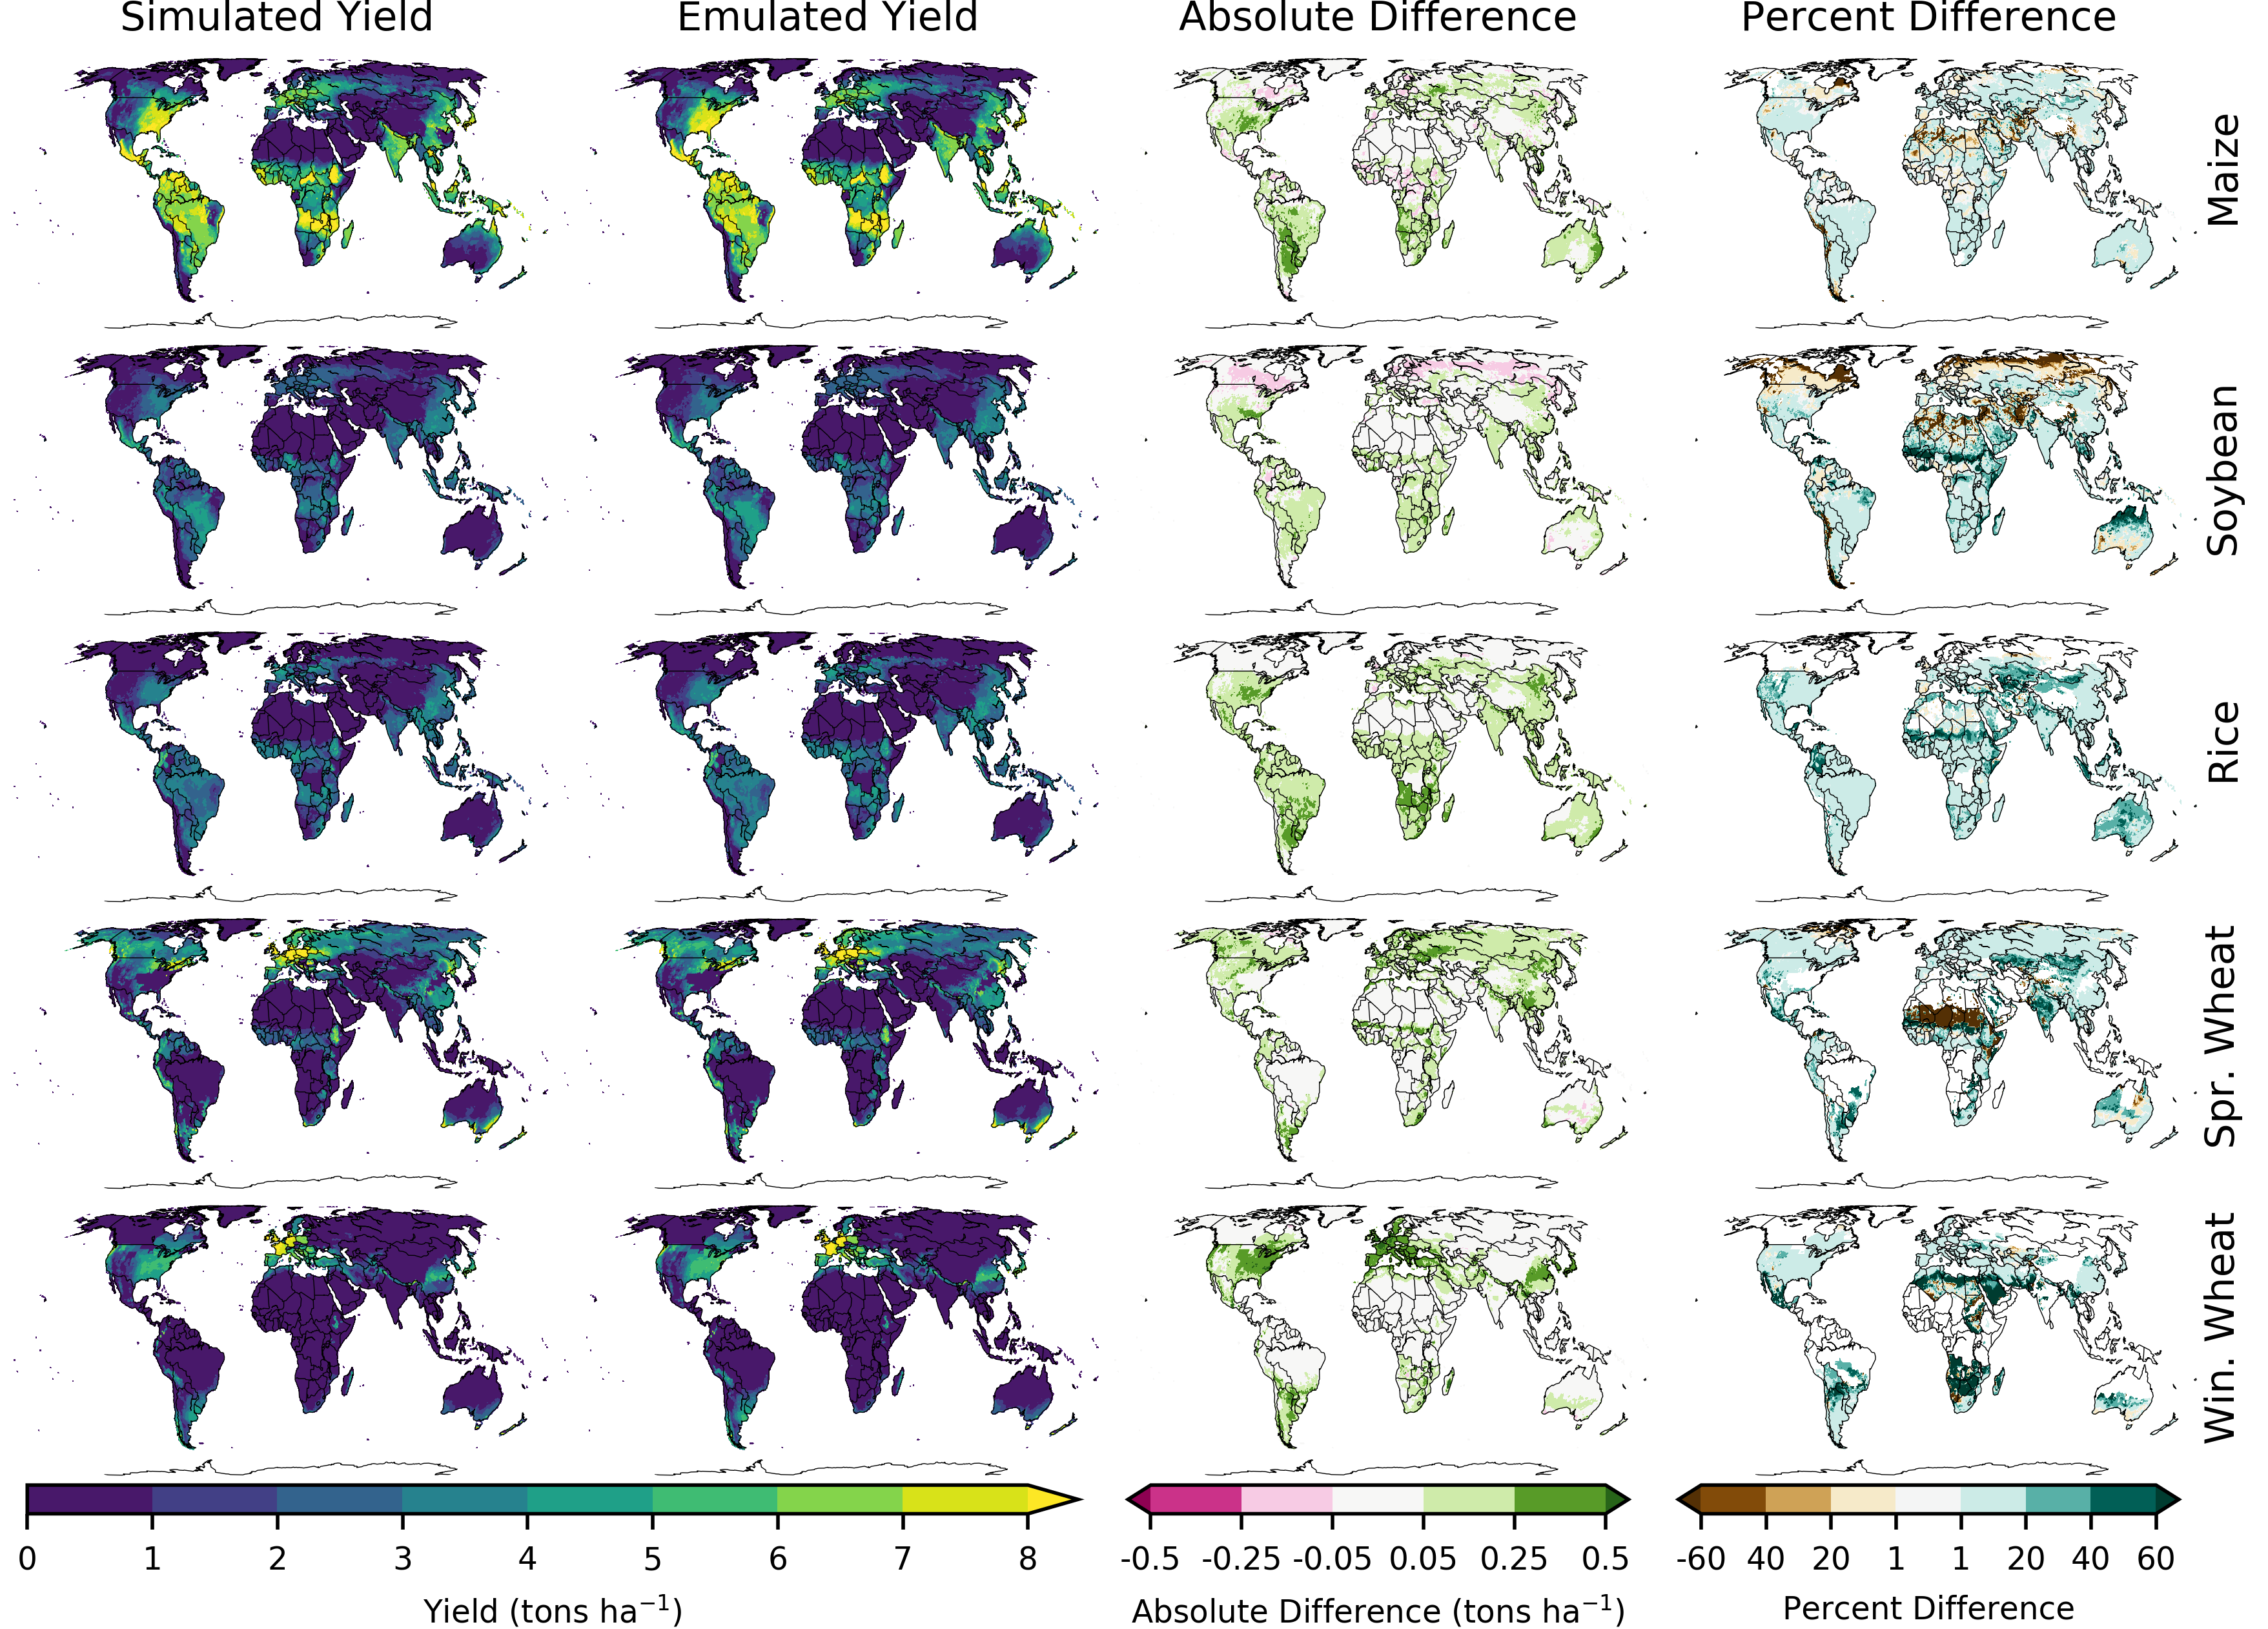
\includegraphics[width=\textwidth]{lpjml_grid.png}
  \caption{Spatial yield response and emulator error for LPJmL for all 5 GGCMI Phase II crops. Convention as in manuscript Figure 4.}
  \label{fig:lpjmlrice}
\end{figure}

\begin{figure}[h!]
  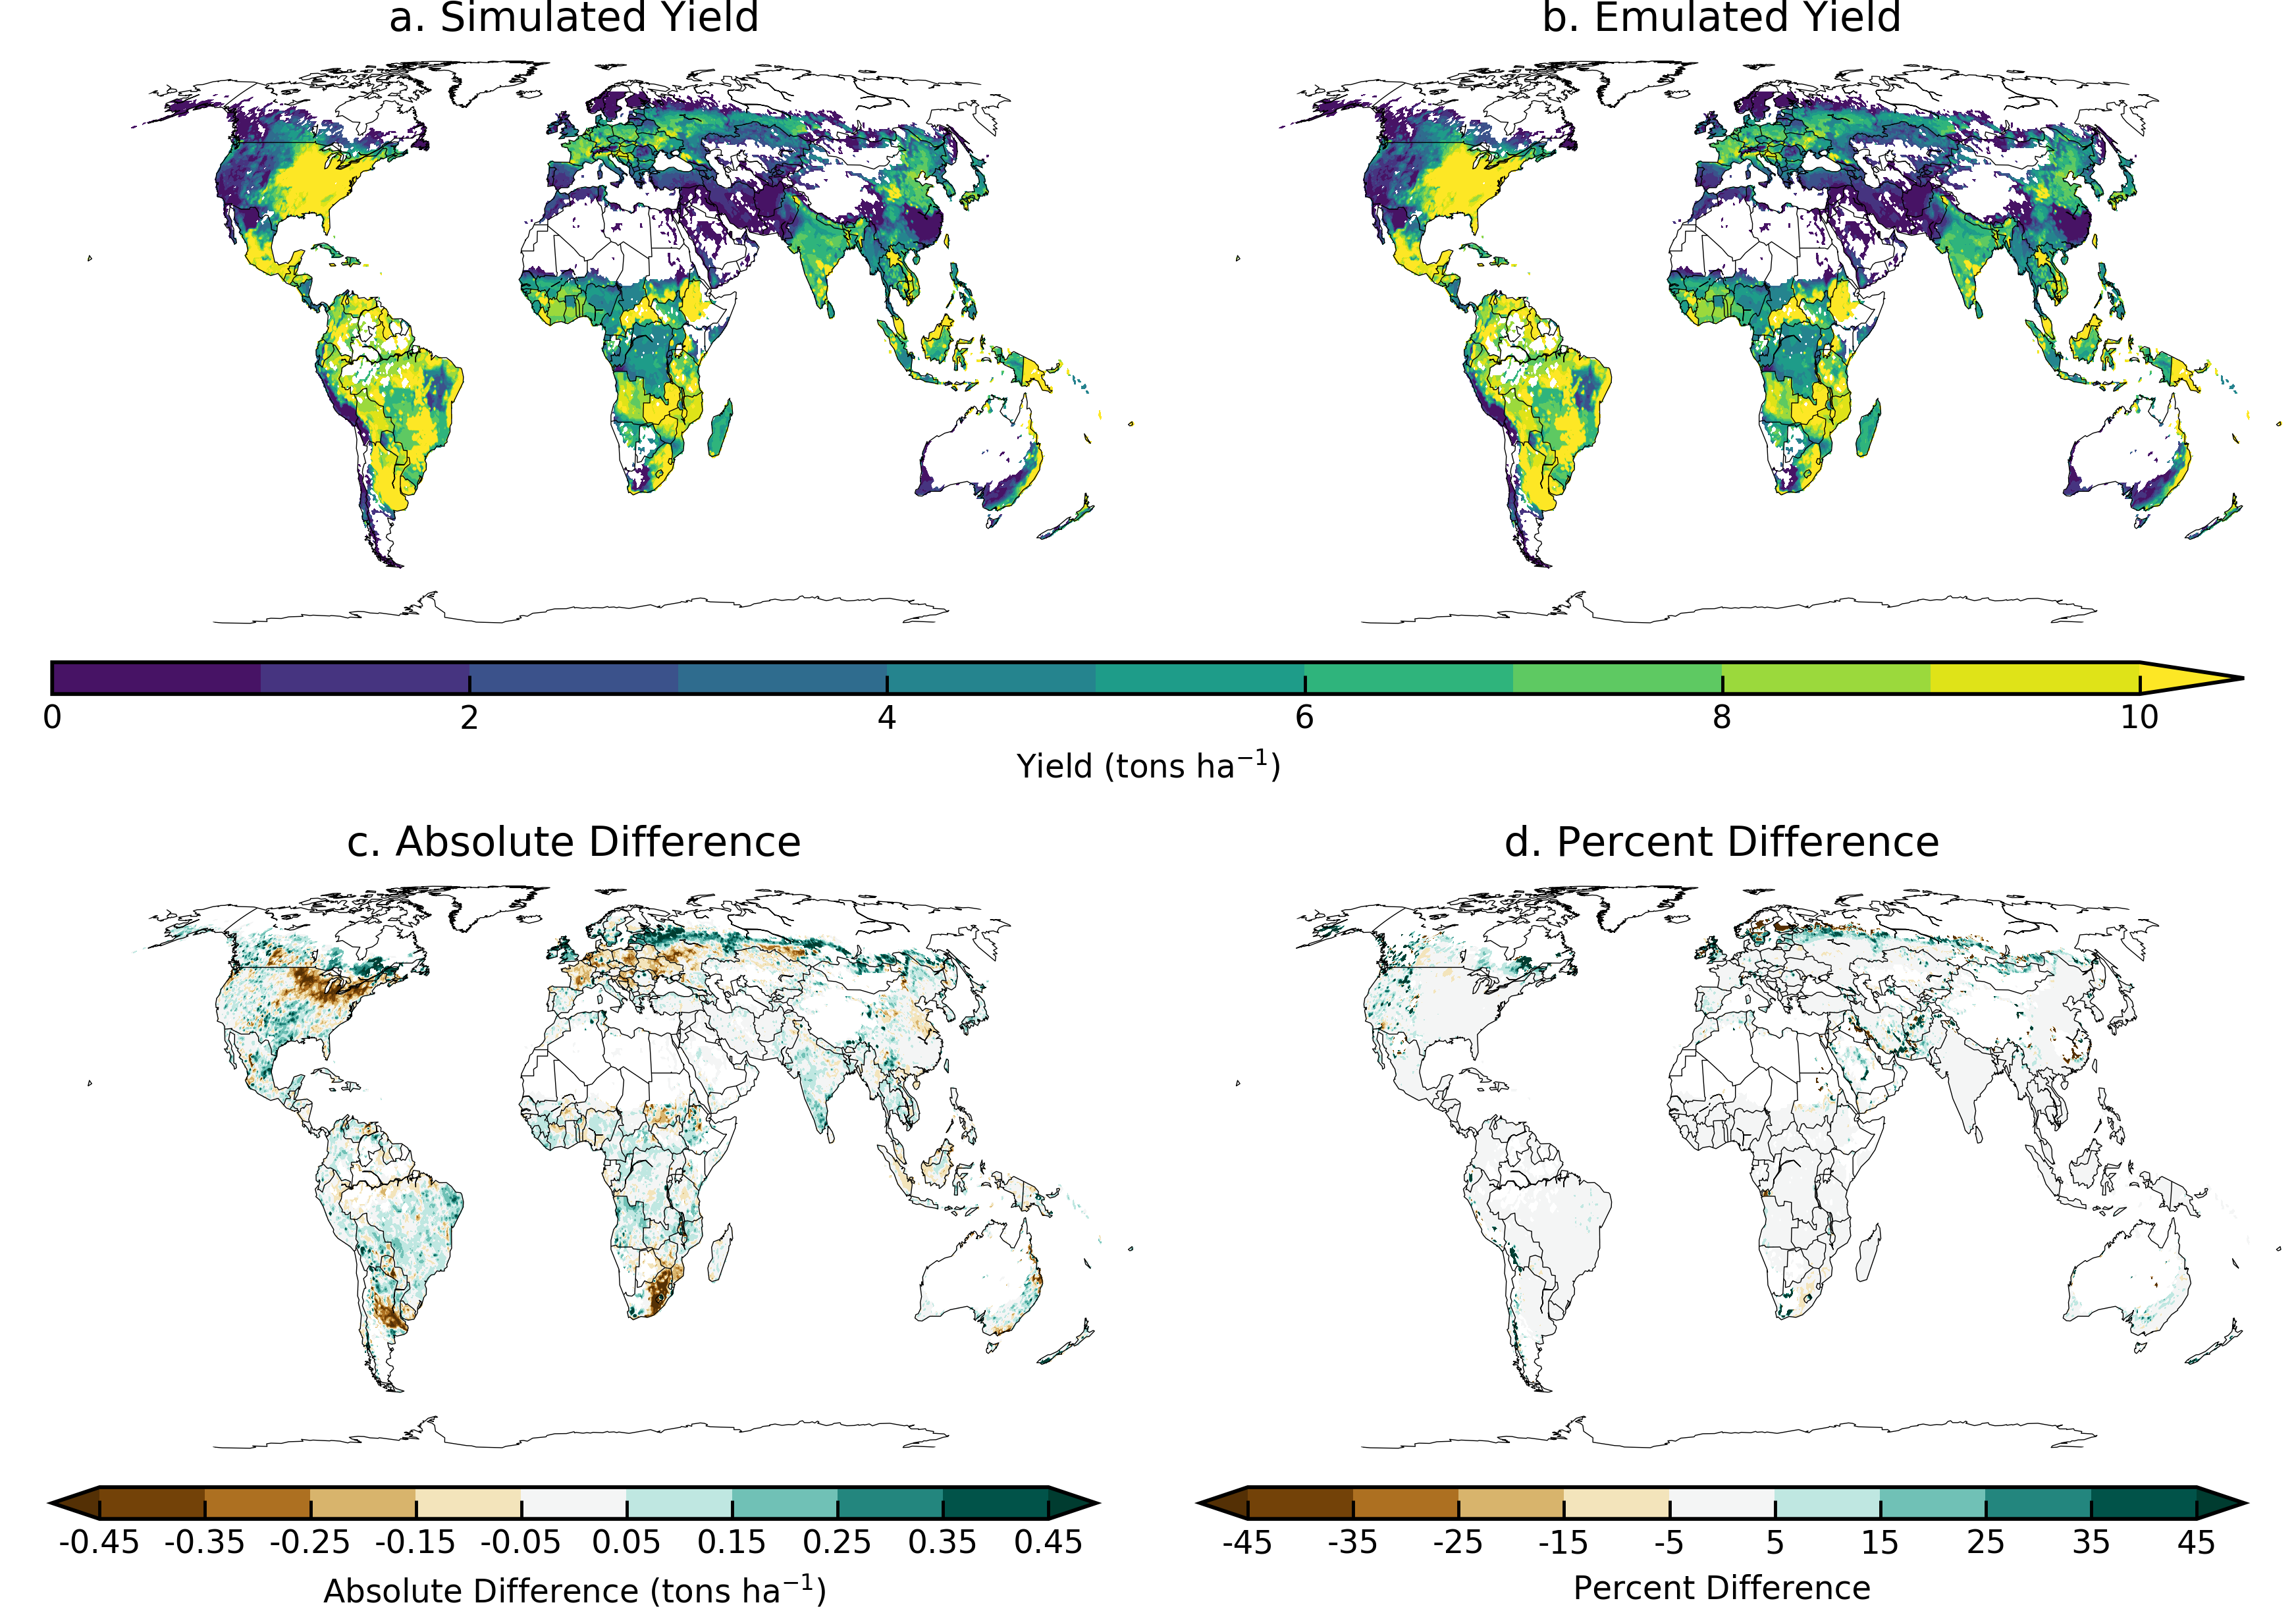
\includegraphics[width=\textwidth]{pdssat_maize.png}
  \caption{Spatial yield response and emulator error for pDSSAT for maize. Convention as in manuscript Figure 4. pDSSAT absolute yields are significantly higher than those in LPJmL but spatial patterns are similar.}
  \label{fig:lpjmlrice}
\end{figure}

%%%%%%%%%%%%%%%%%%%%%%%%%%%%%%%%%%%%%%%%%%%%%%%%%%%%%%%%%%%%%%%%%%%%%%%%%%%%%%%%%%%%%%%
%%%%%%%%%%%%%%%%%%%%%%%%%%%%%%%%%%%%%%%%%%%%%%%%%%%%%%%%%%%%%%%%%%%%%%%%%%%%%%%%%%%%%%%
%%%%%%%%%%%%%%%%%%%%%%%%%%%%%%%%%%%%%%%%%%%%%%%%%%%%%%%%%%%%%%%%%%%%%%%%%%%%%%%%%%%%%%%
\clearpage
\section{Cross validation error for all models}
\begin{justify}
In this section we present maps of cross validation error (values found in main text Table 3 are aggregated up from the grid cell level). Errors are generally low as a percentage of yield change in each grid cell.
Errors above 10\% of yield change in the out-of-sample test occur very rarely; the only significant instance is spring wheat in southern China in the PROMET model.
\end{justify}

\begin{figure}[!htb]
  \centering
  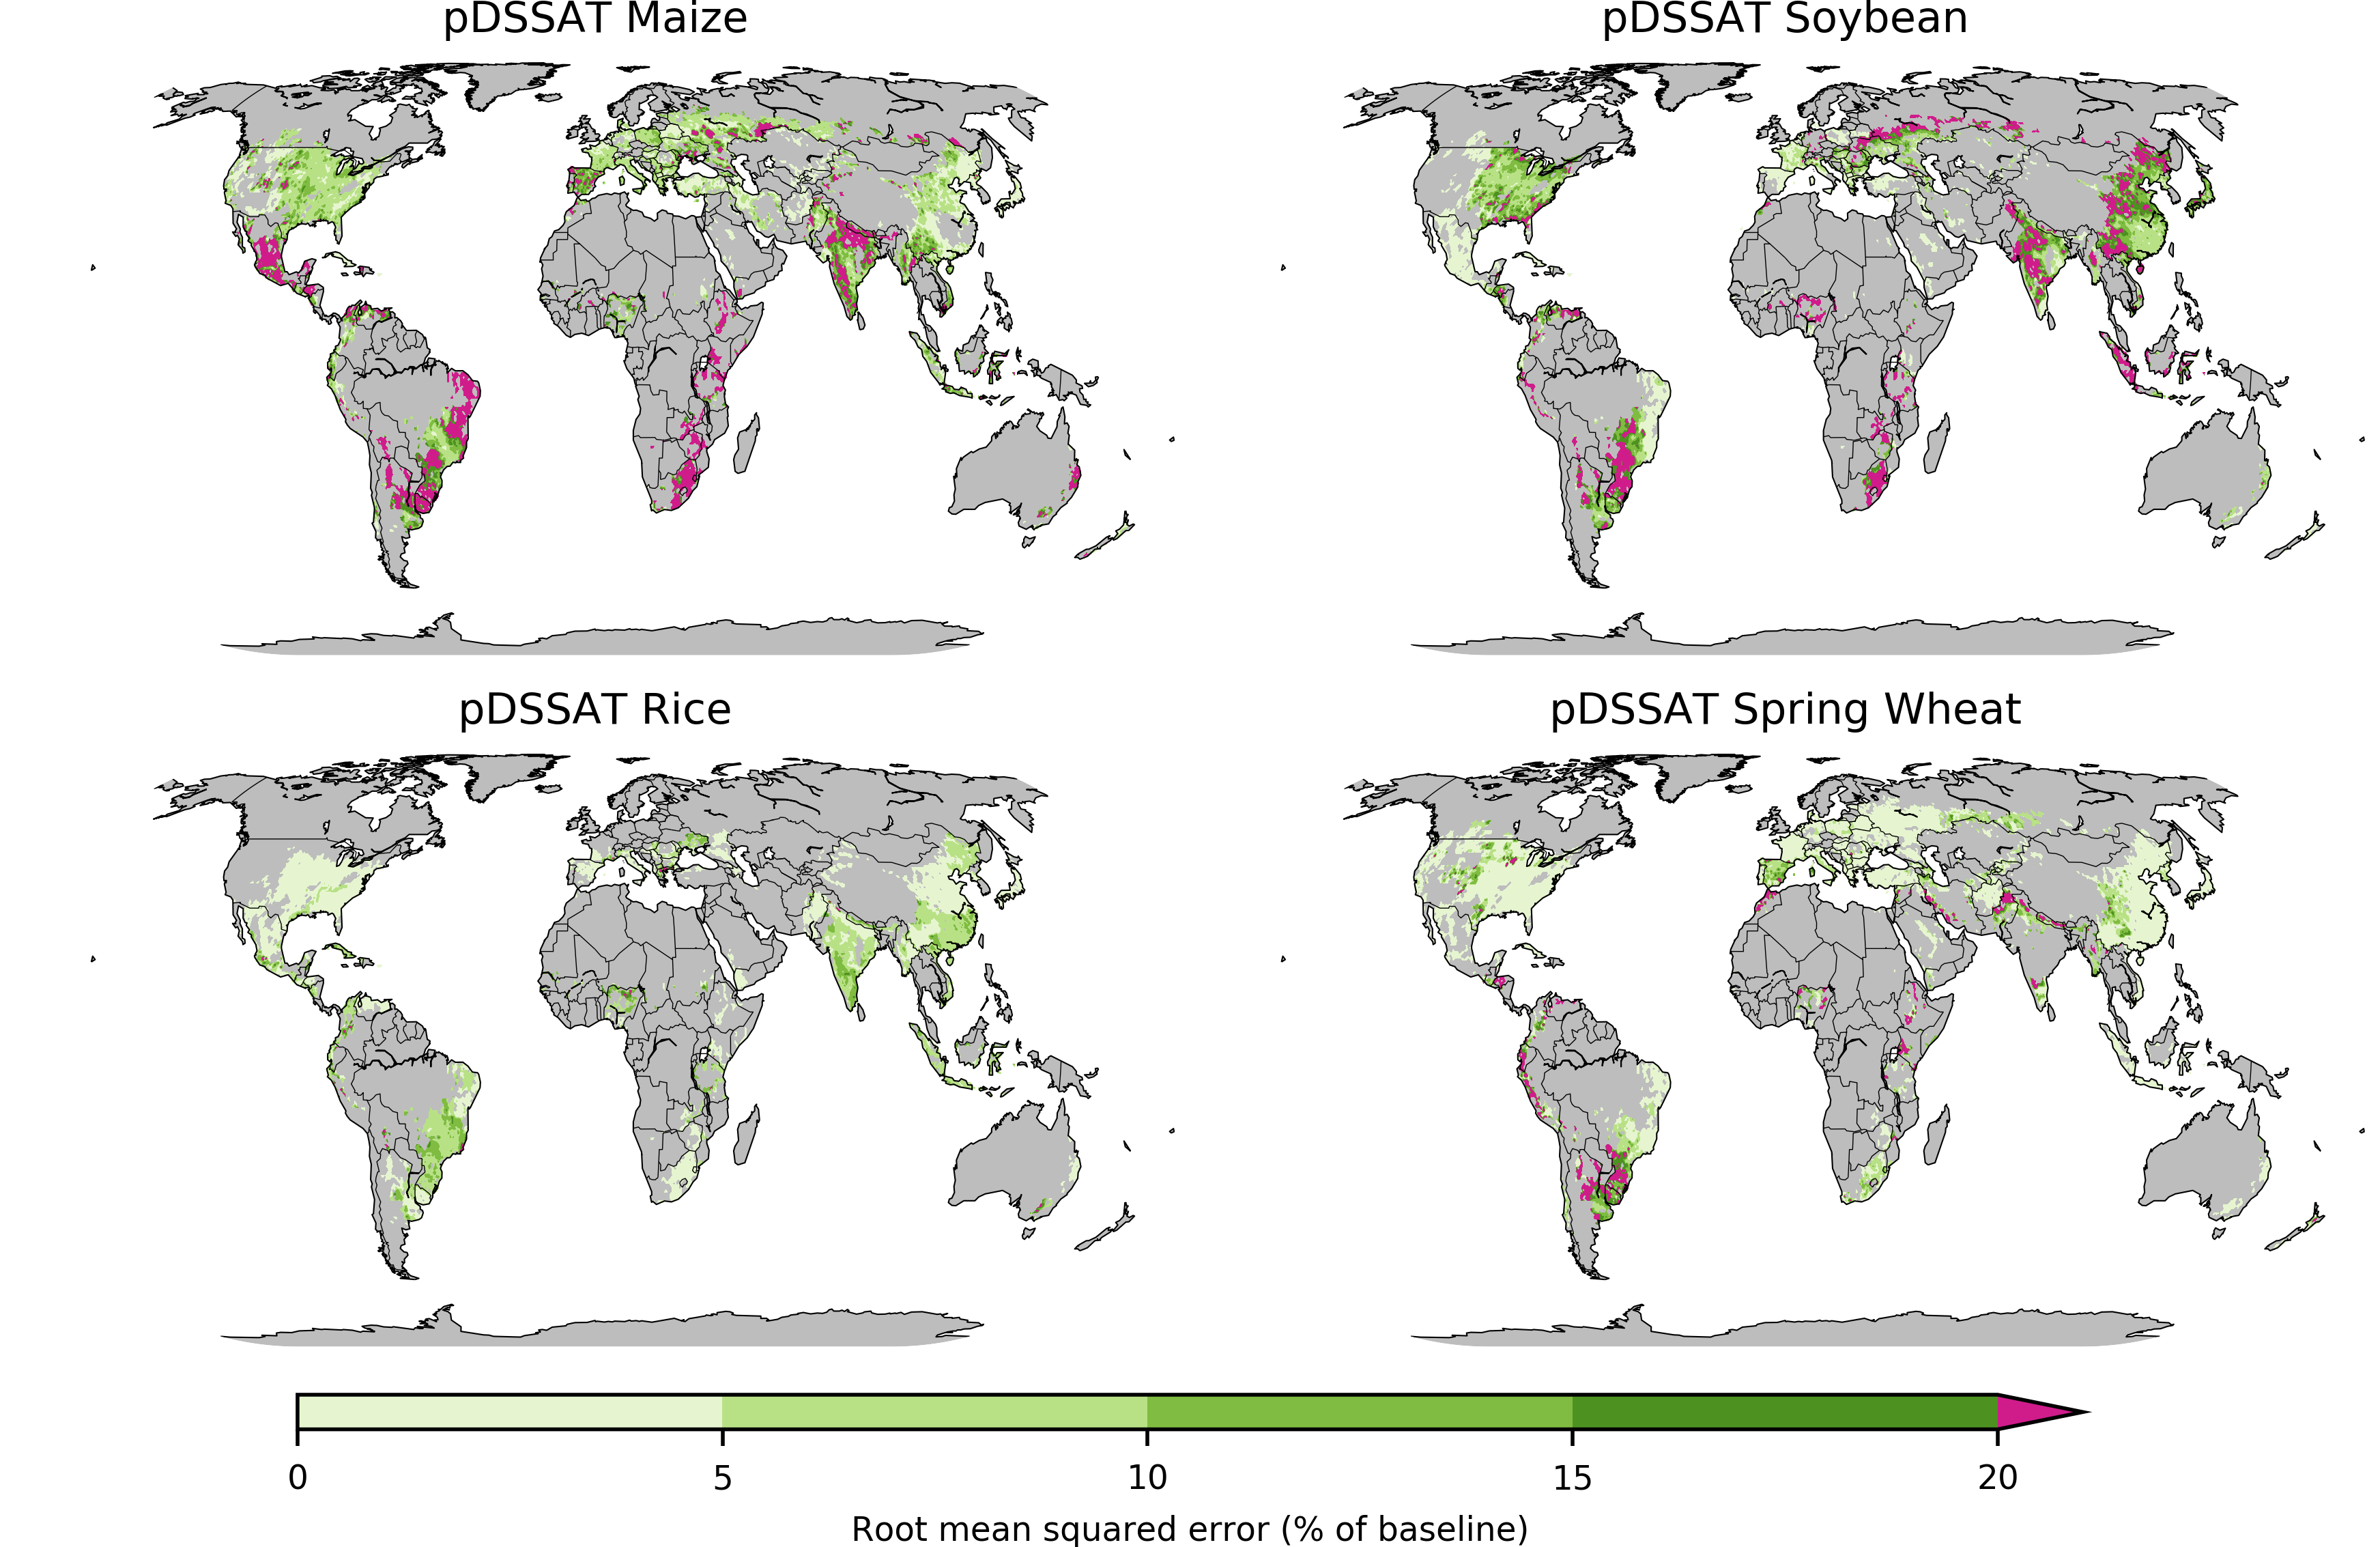
\includegraphics[width=15.5cm]{pDSSAT_spatial_MSE_ton_ha.png}
  \caption{Root mean squared error for cross validation for the pDSSAT model for rainfed crops. Values shown as a percentage of yield change in each grid cell.}
\end{figure}

\begin{figure}[!htb]
  \centering
  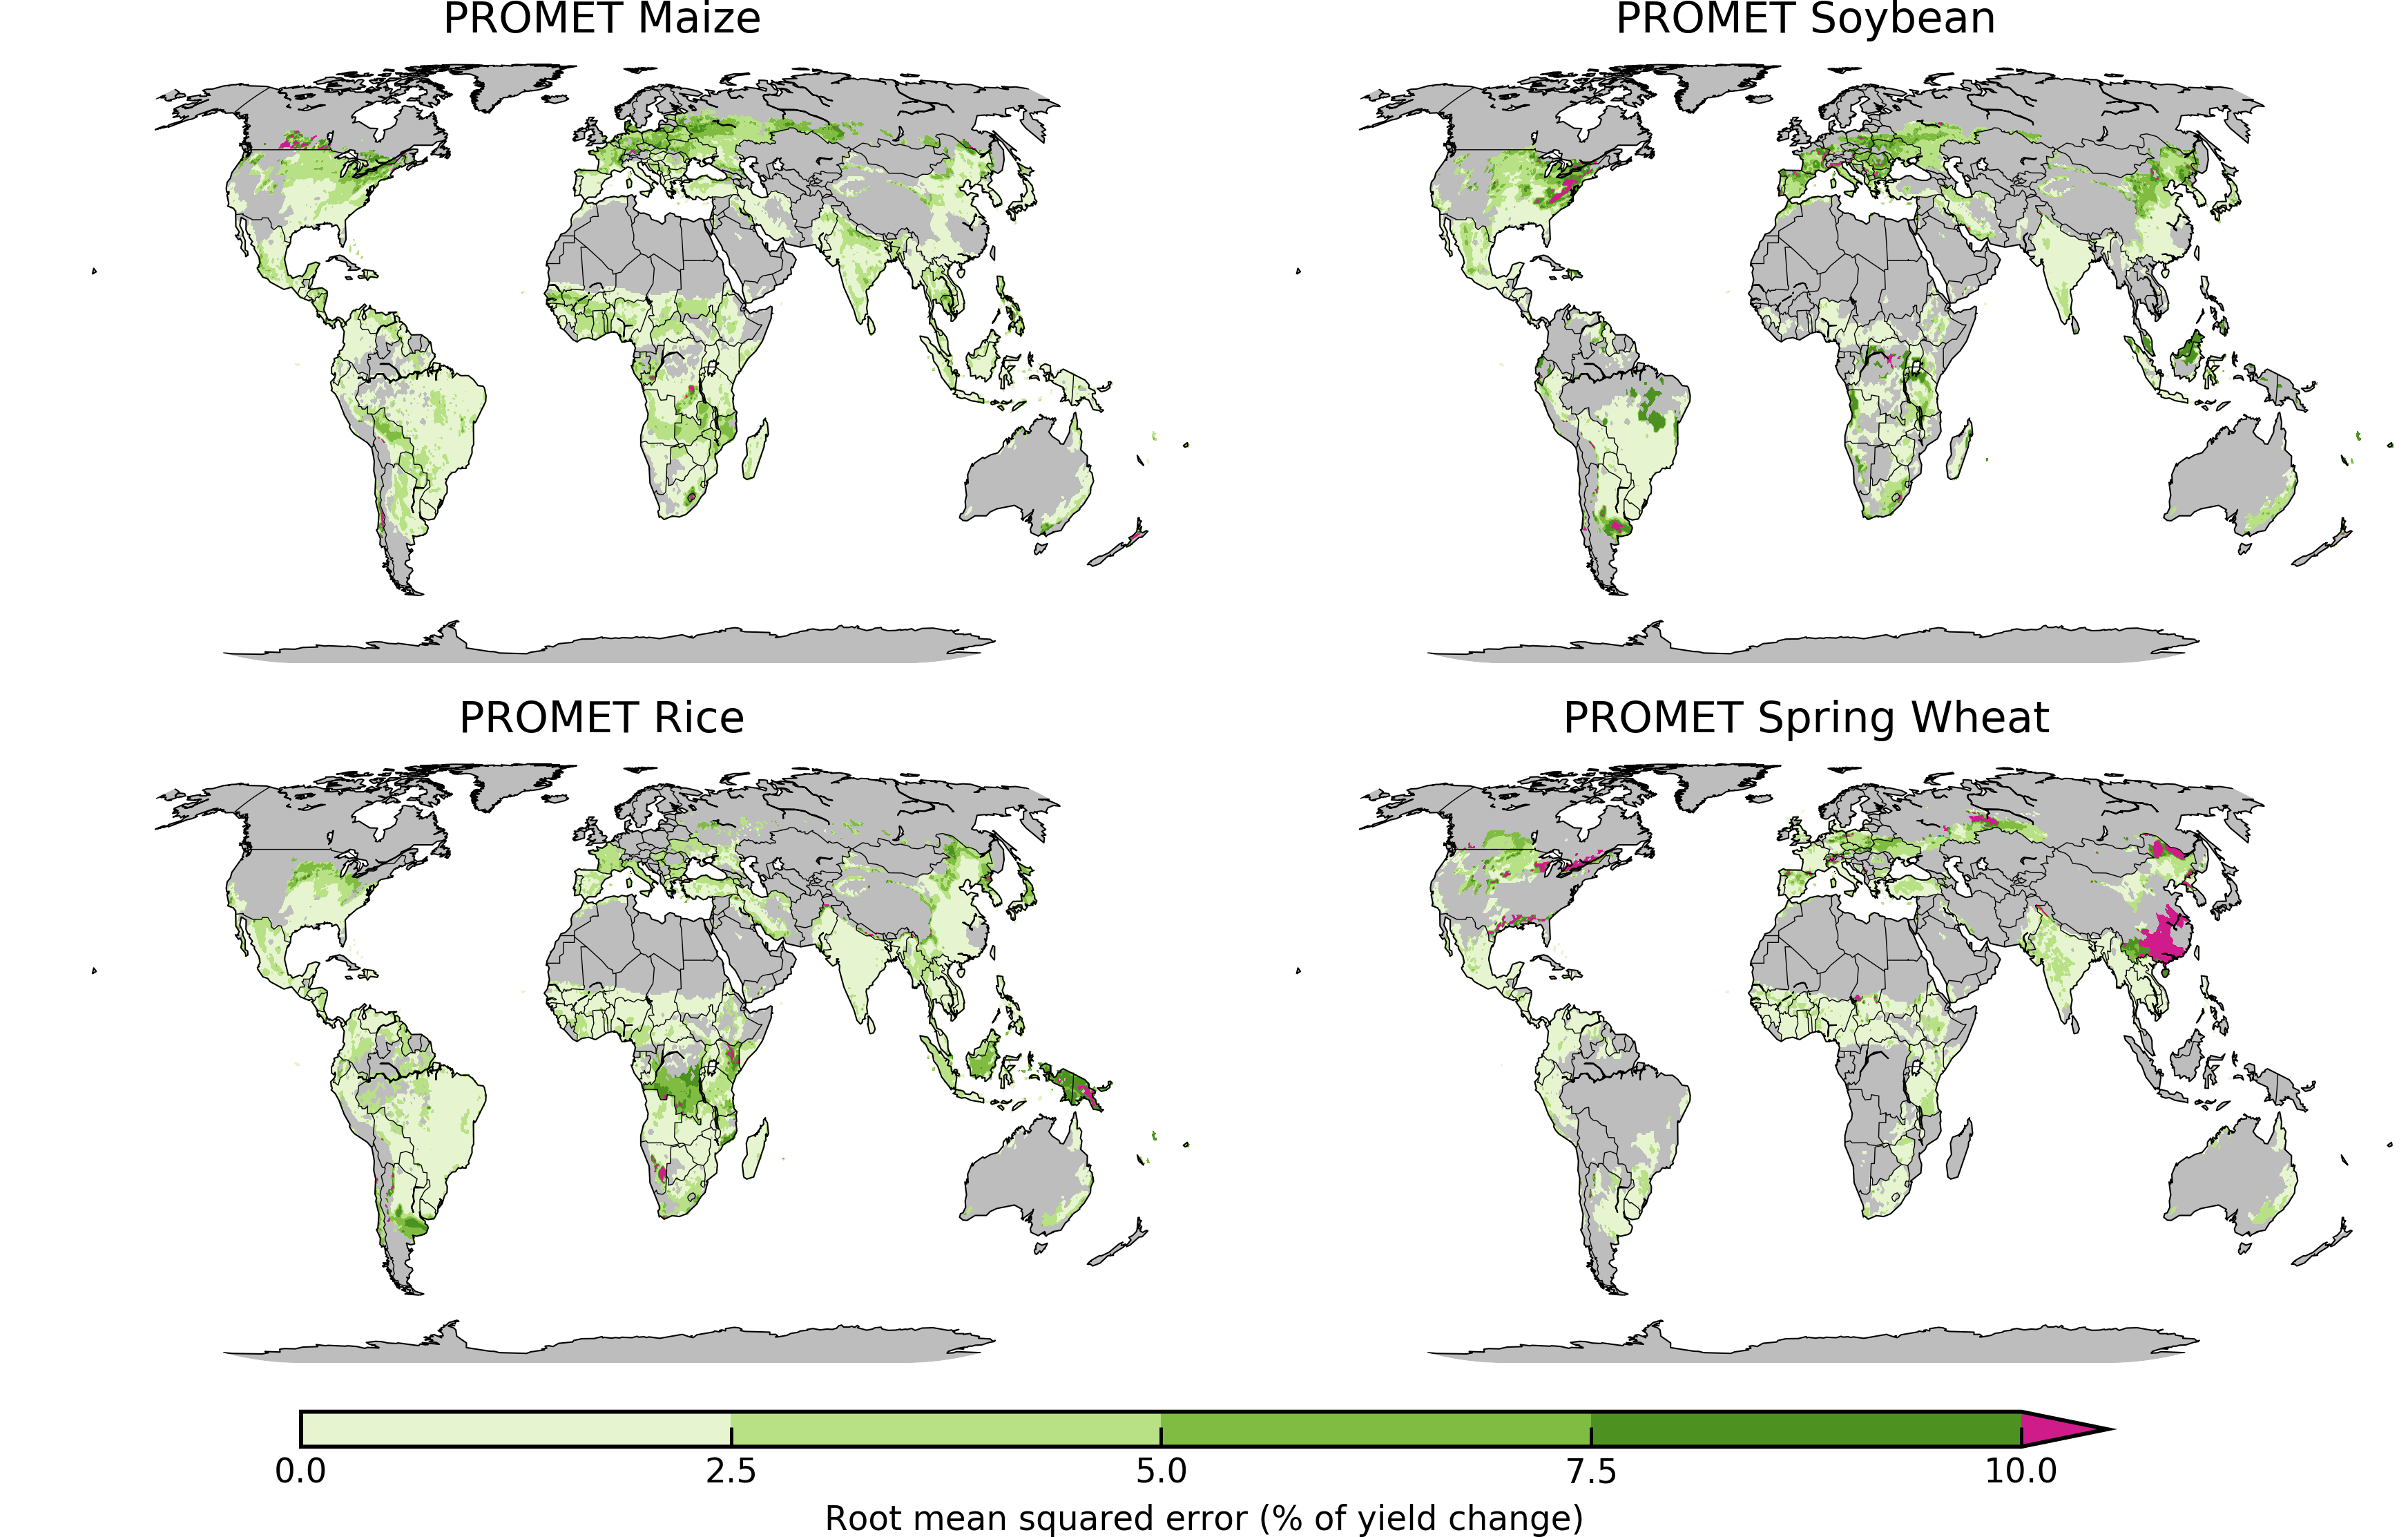
\includegraphics[width=15.5cm]{PROMET_spatial_MSE_ton_ha.png}
  \caption{Map of root mean squared error for cross validation process for the PROMET model for rainfed crops. Values shown as a percentage of yield change in each grid cell.}
\end{figure}

\begin{figure}[!htb]
  \centering
  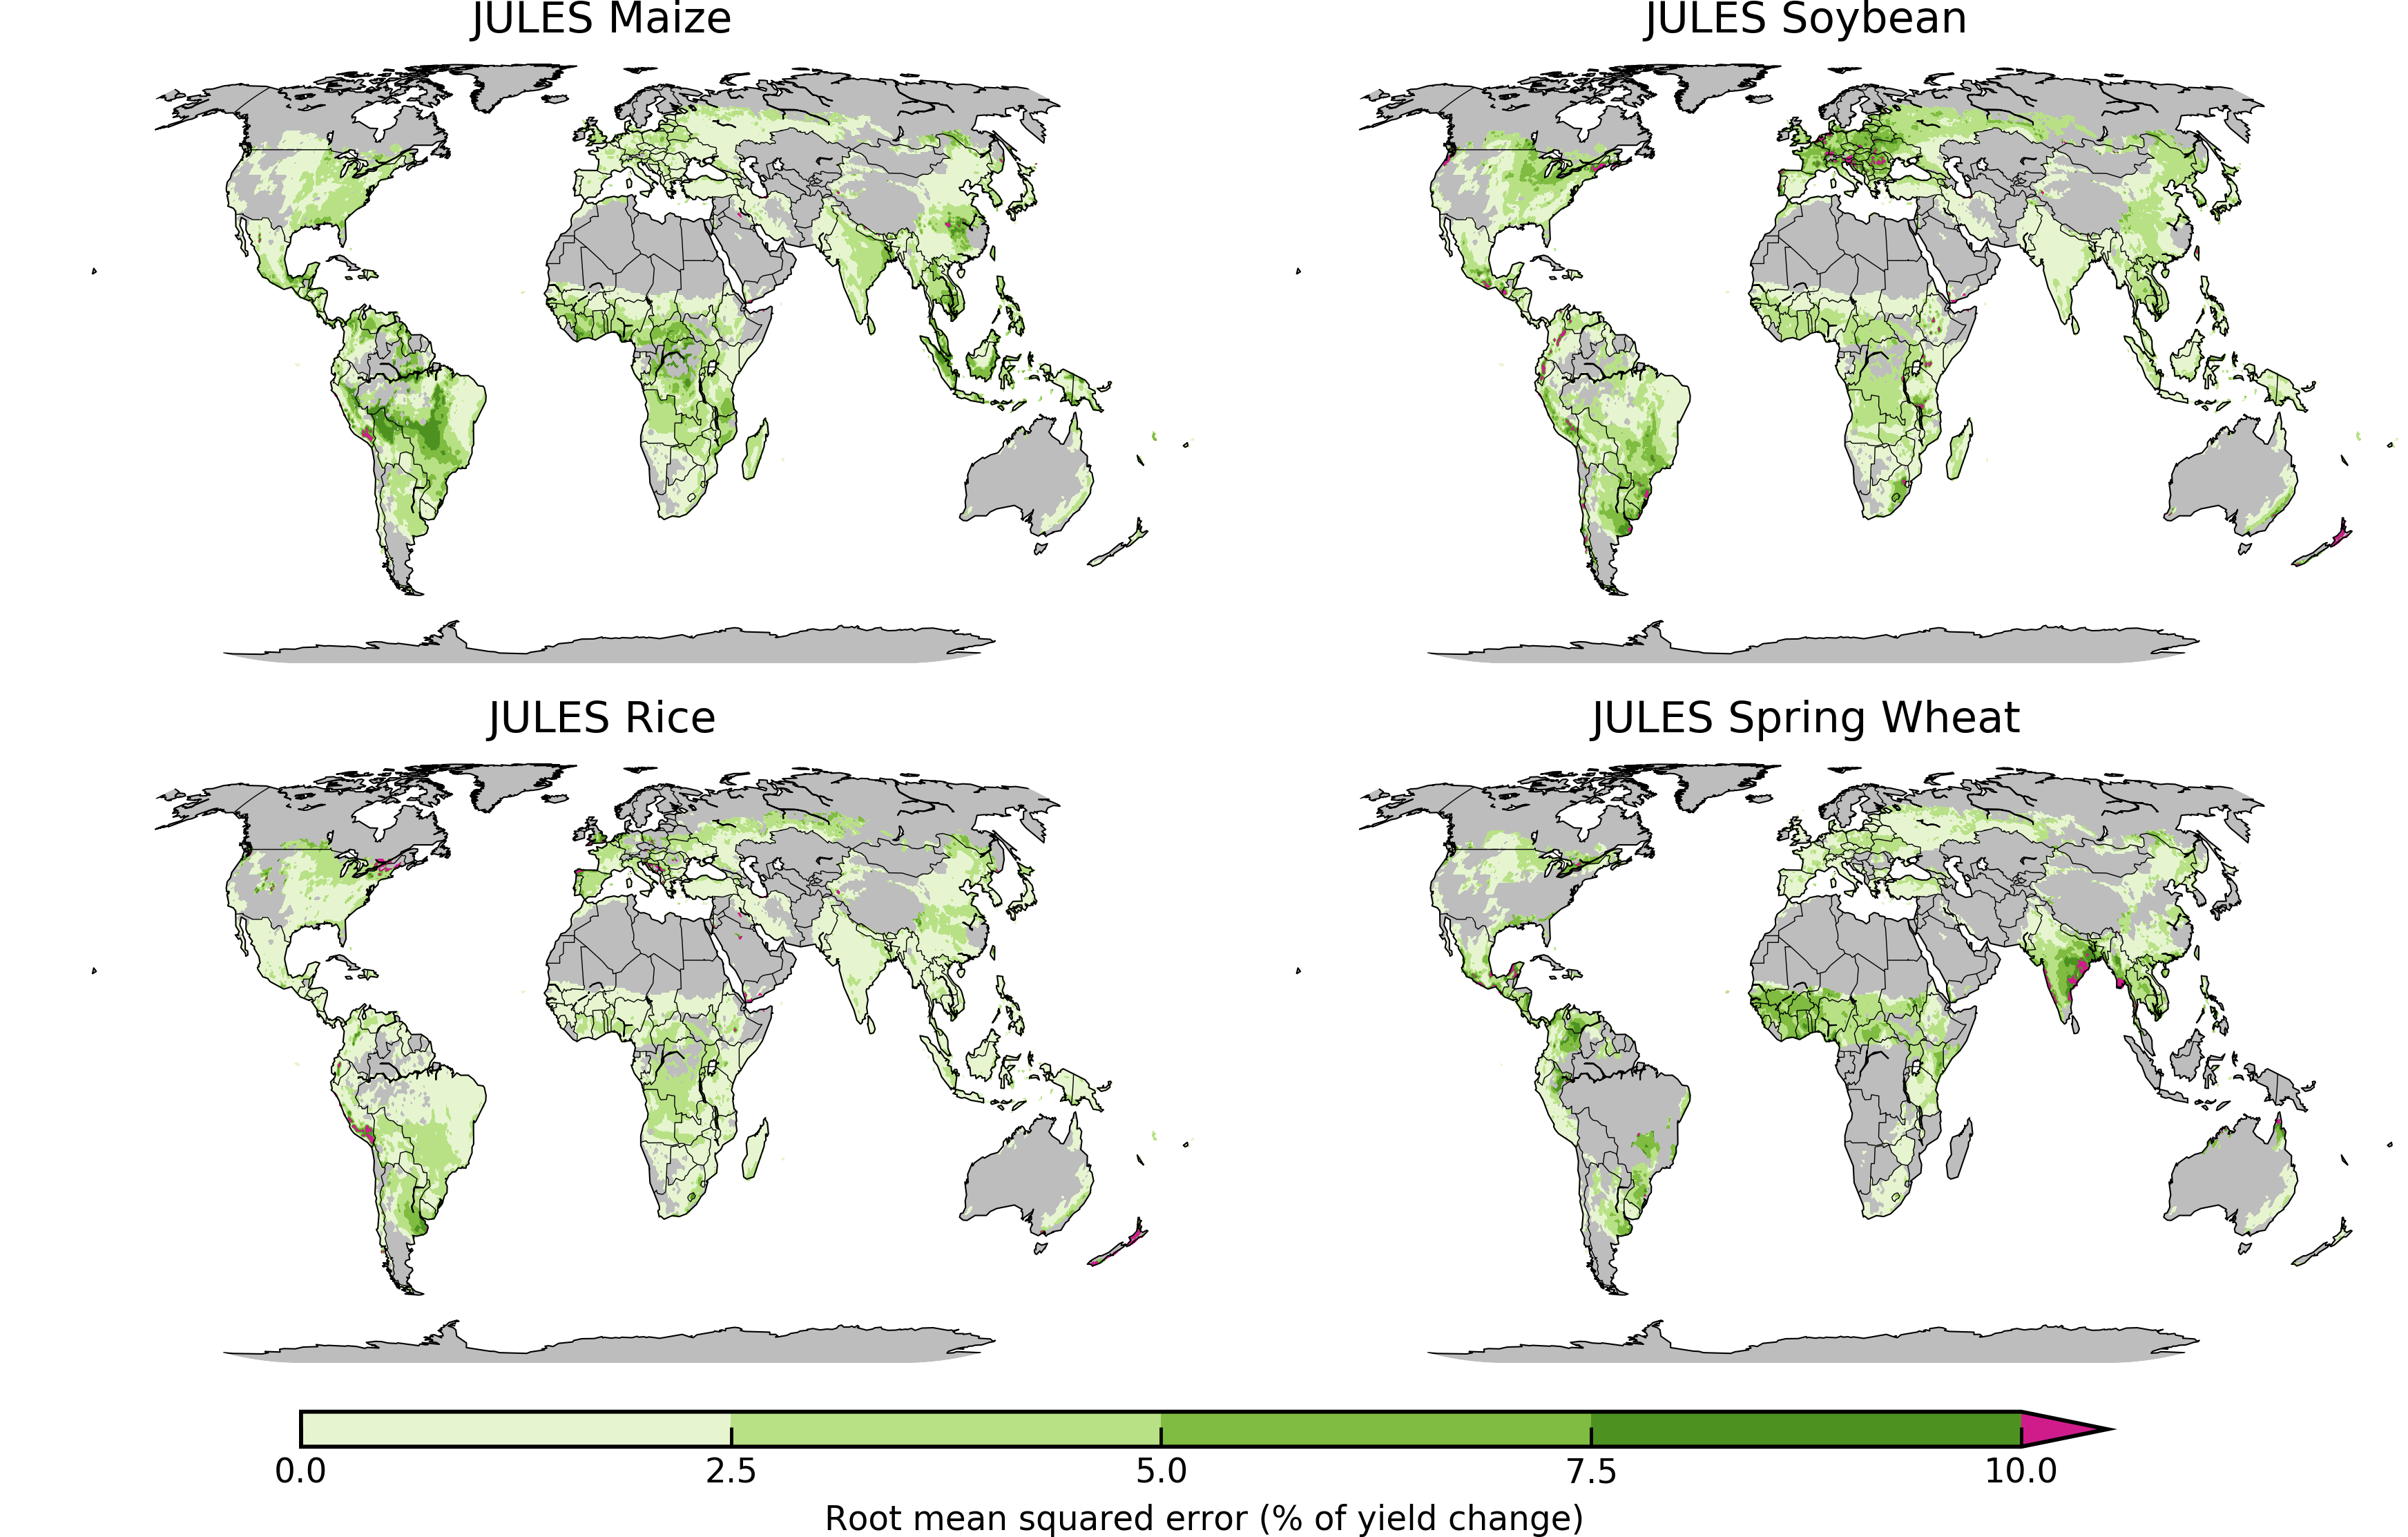
\includegraphics[width=15.5cm]{JULES_spatial_MSE_ton_ha.png}
  \caption{Map of root mean squared error for cross validation process for the JULES model for rainfed crops. Values shown as a percentage of yield change in each grid cell.}
\end{figure}

\begin{figure}[!htb]
  \centering
  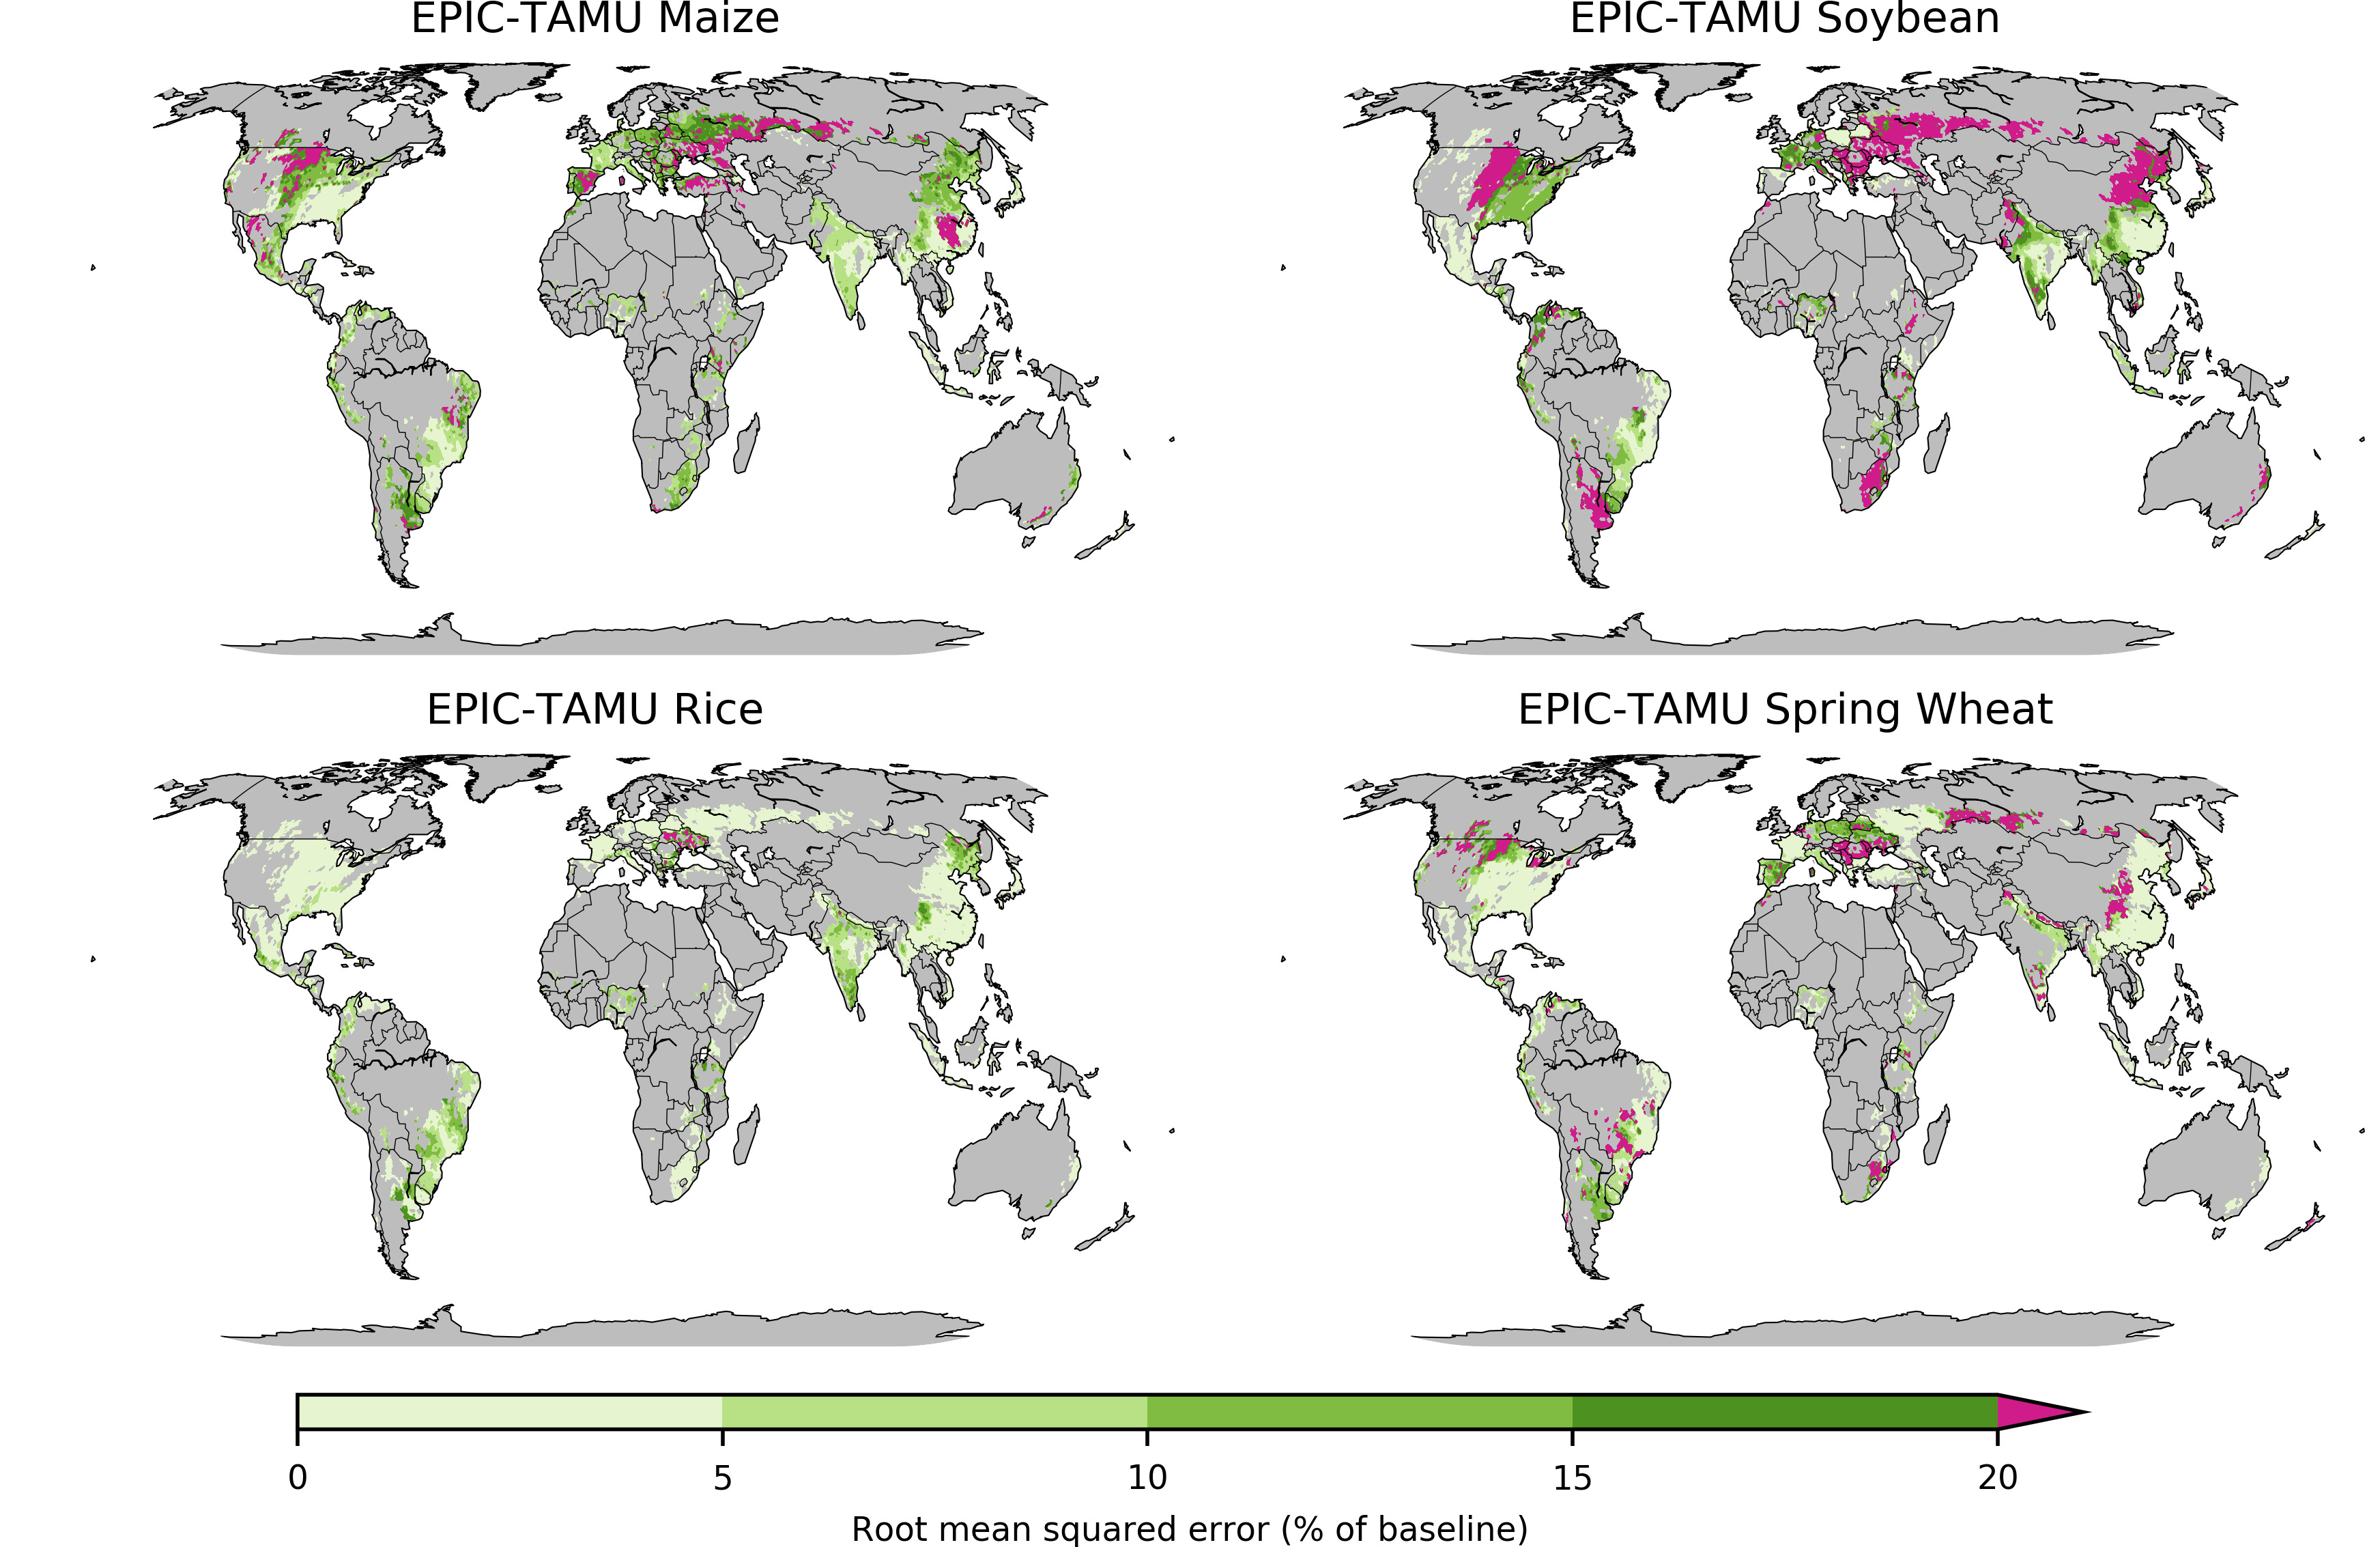
\includegraphics[width=15.5cm]{EPIC-TAMU_spatial_MSE_ton_ha.png}
  \caption{Map of root mean squared error for cross validation process for the EPIC-TAMU model for rainfed crops. Values shown as a percentage of yield change in each grid cell.}
\end{figure}

\begin{figure}[!htb]
  \centering
  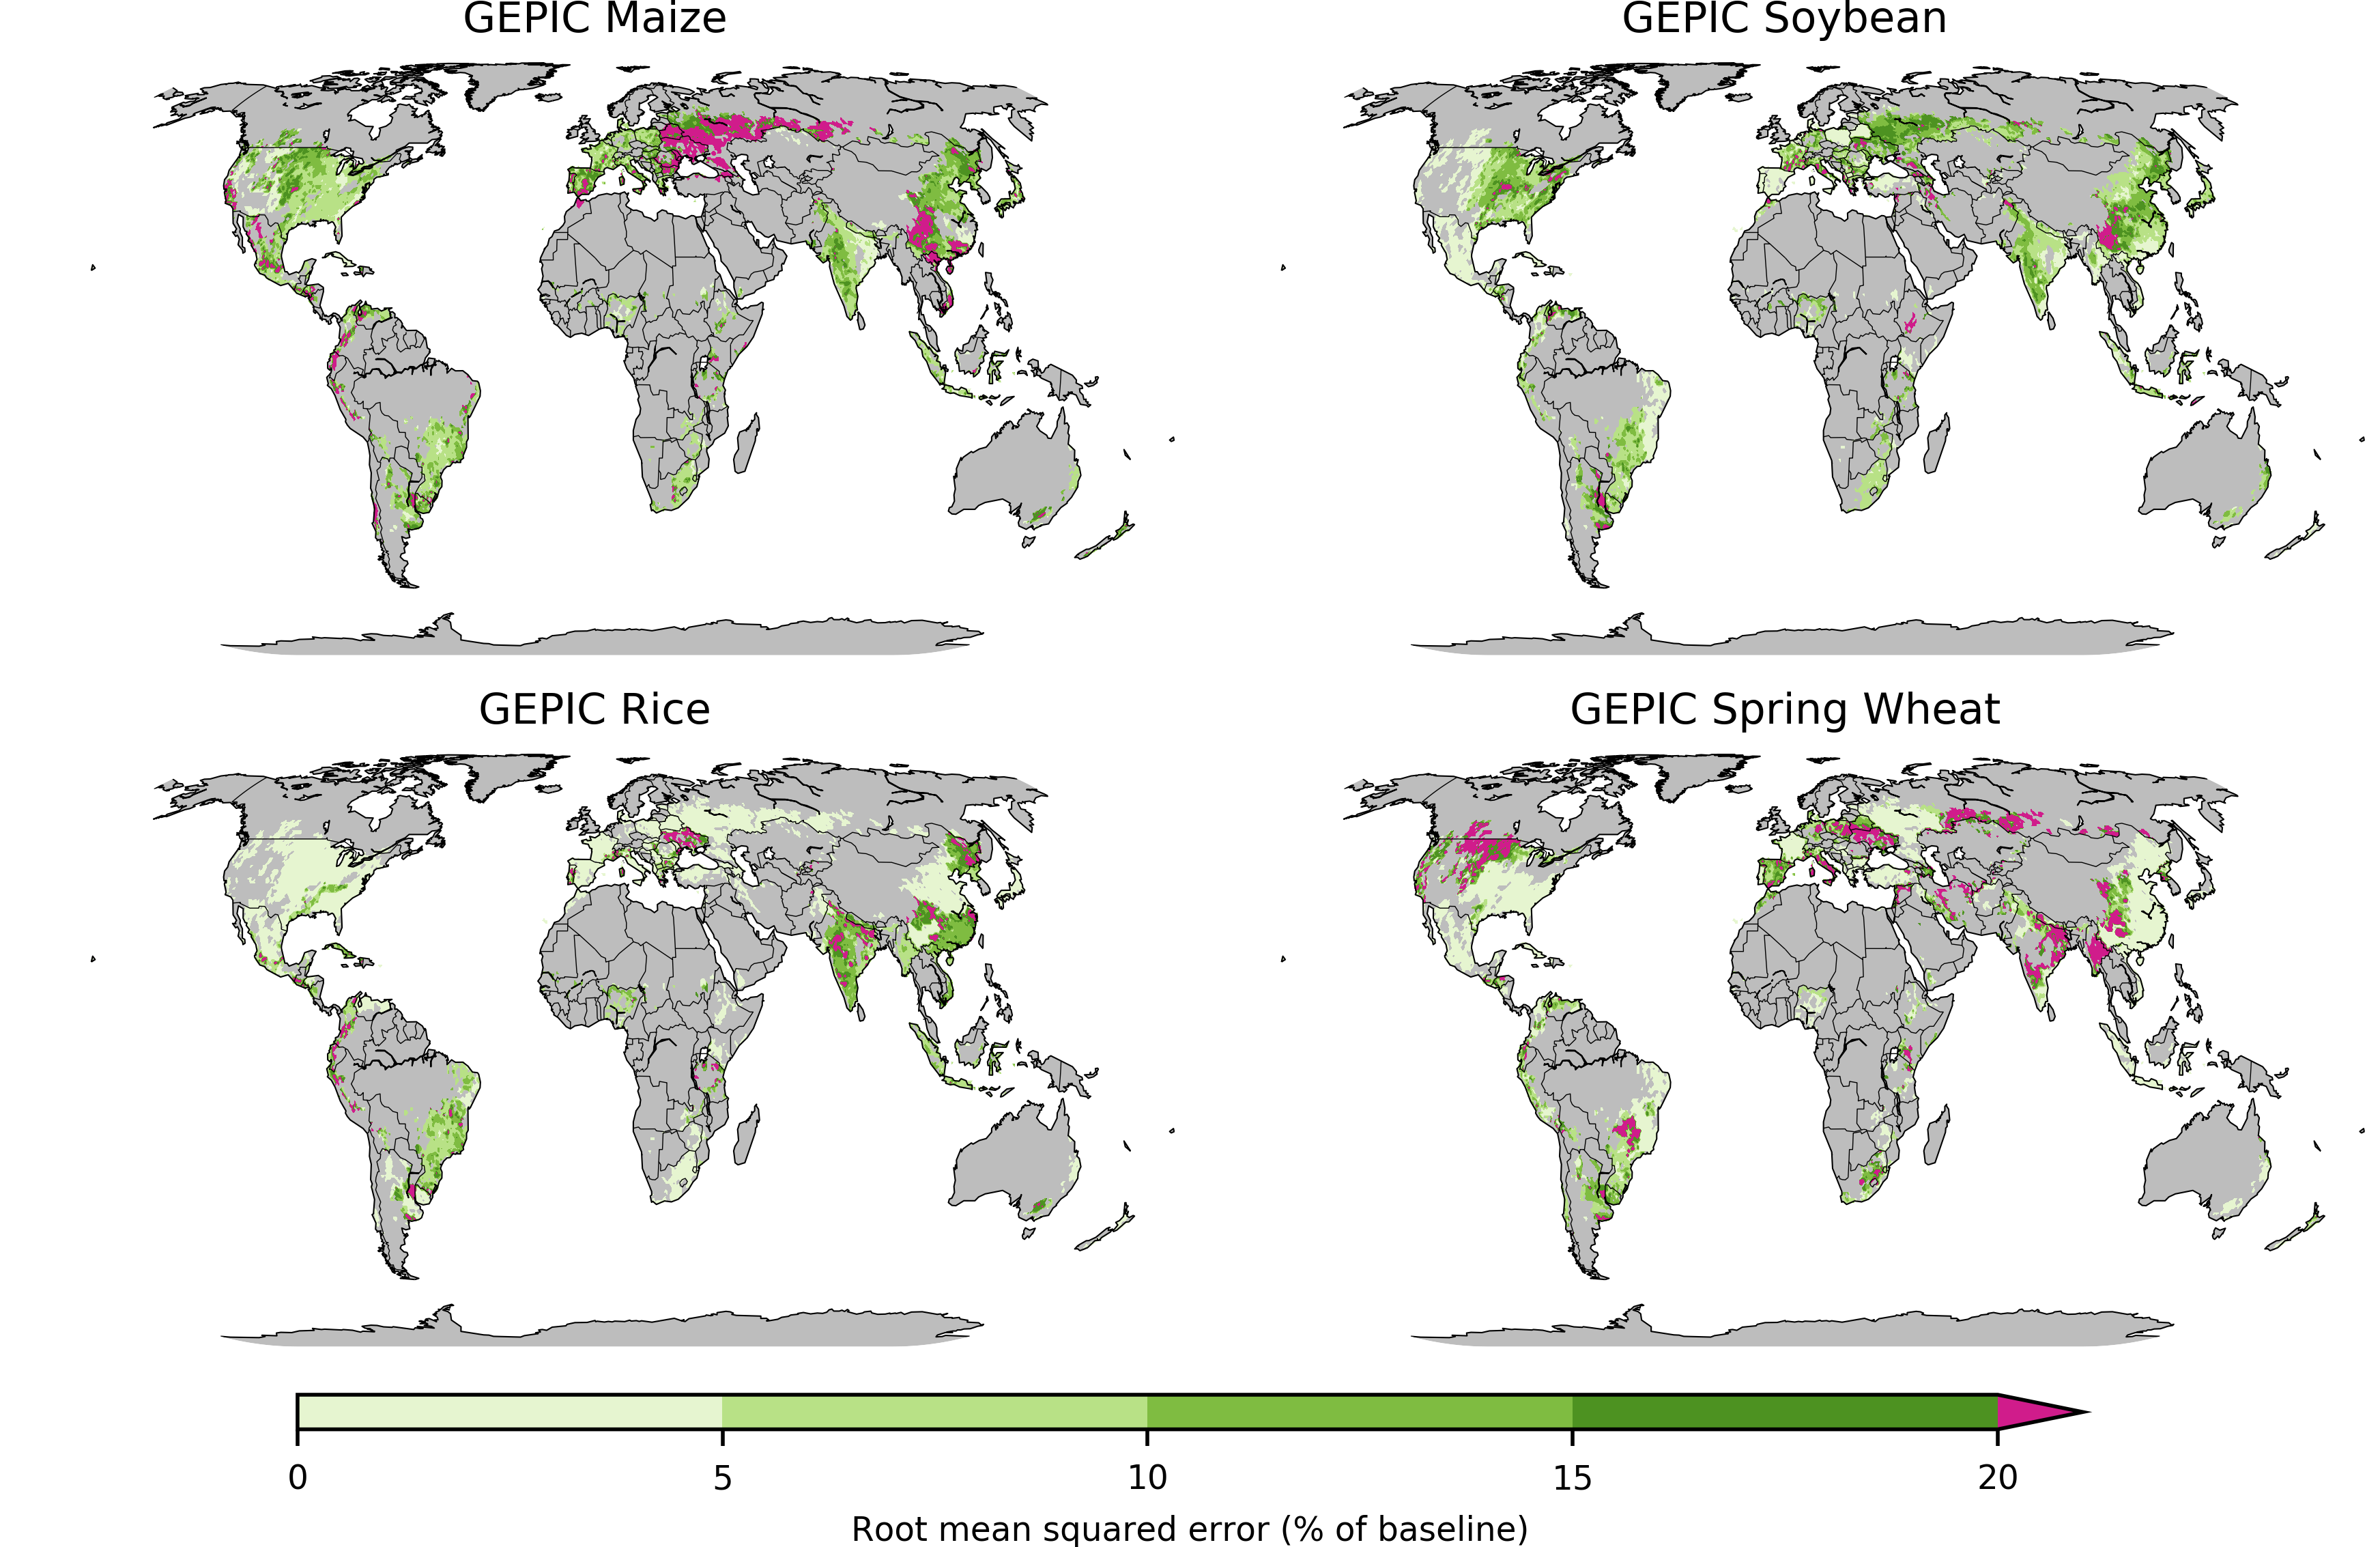
\includegraphics[width=15.5cm]{GEPIC_spatial_MSE_ton_ha.png}
  \caption{Map of root mean squared error for cross validation process for the GEPIC model for rainfed crops. Values shown as a percentage of yield change in each grid cell.}
\end{figure}

\begin{figure}[!htb]
  \centering
  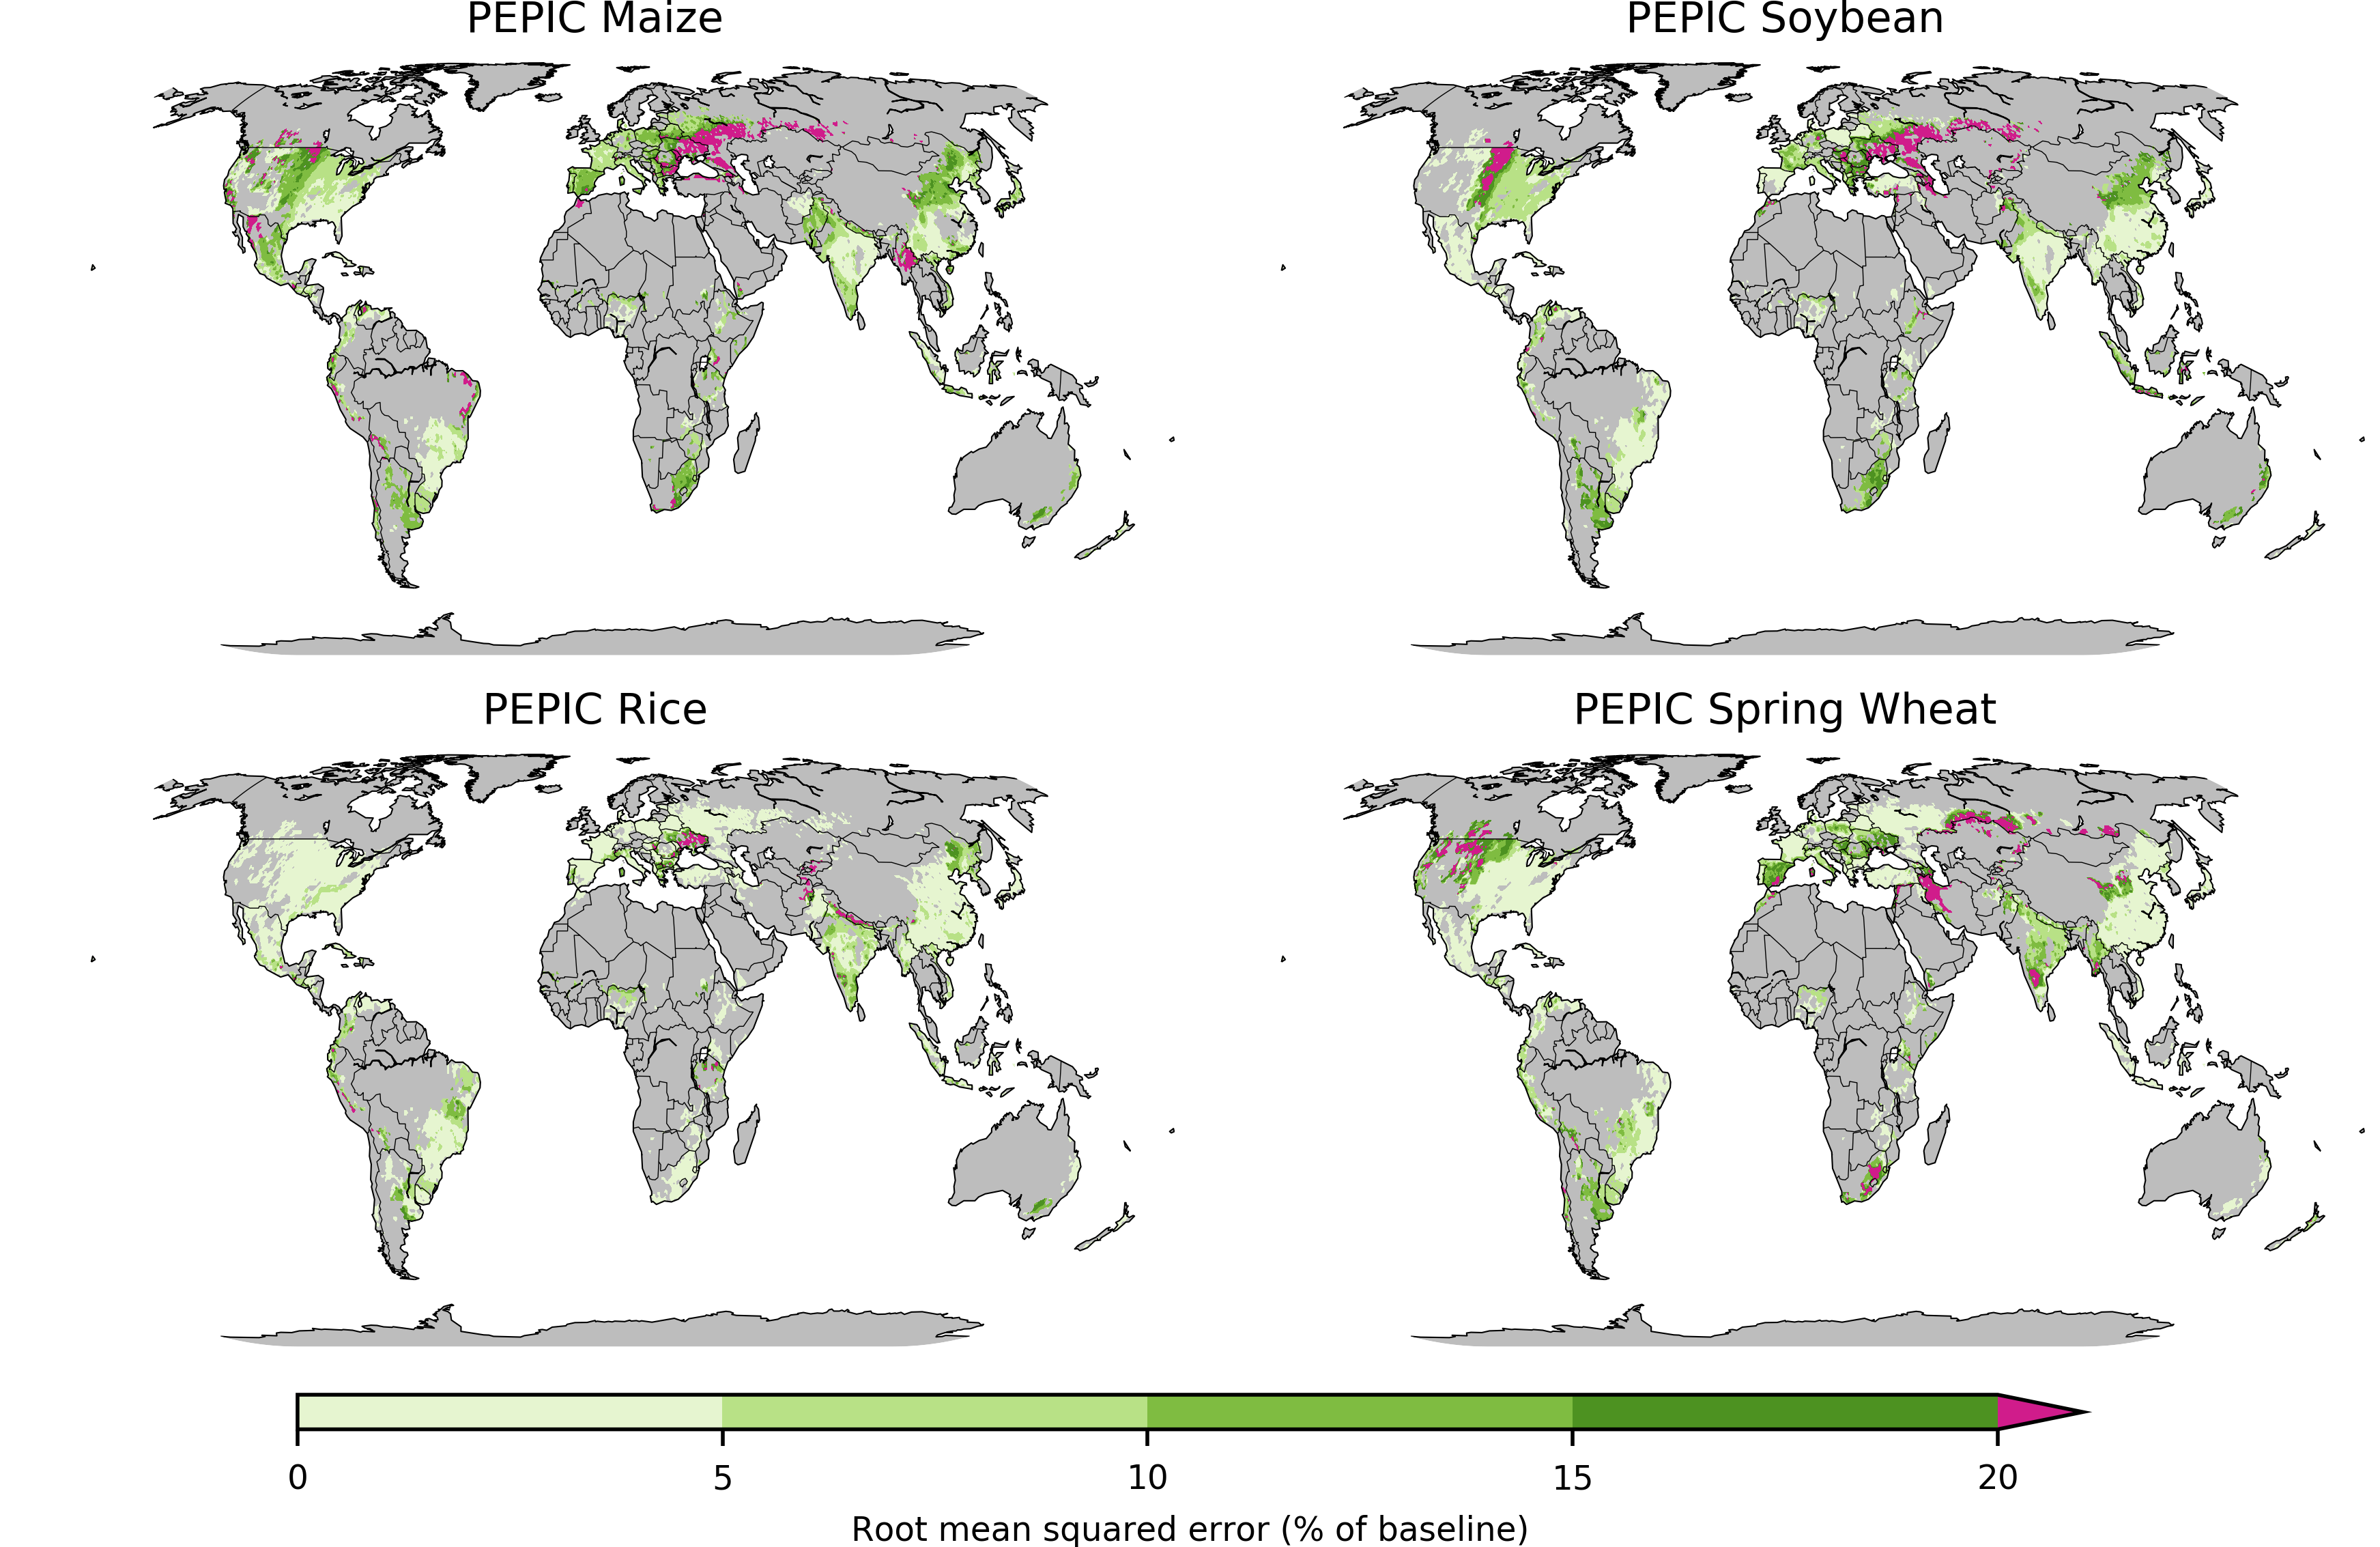
\includegraphics[width=15.5cm]{PEPIC_spatial_MSE_ton_ha.png}
  \caption{Map of root mean squared error for cross validation process for the PEPIC model for rainfed crops. Values shown as a percentage of yield change in each grid cell.}
\end{figure}

\clearpage
%\bibliography{bib}
\printbibliography
%\bibliographystyle{Plain}

\end{document}




\clearpage
\section{Normalized Error for all models}
\begin{justify}
For completeness, this section provides maps of normalized error $e$ with the same convention as manuscript Figure 8 text for all models. 
\end{justify}

\begin{figure}[h!]
  \centering
  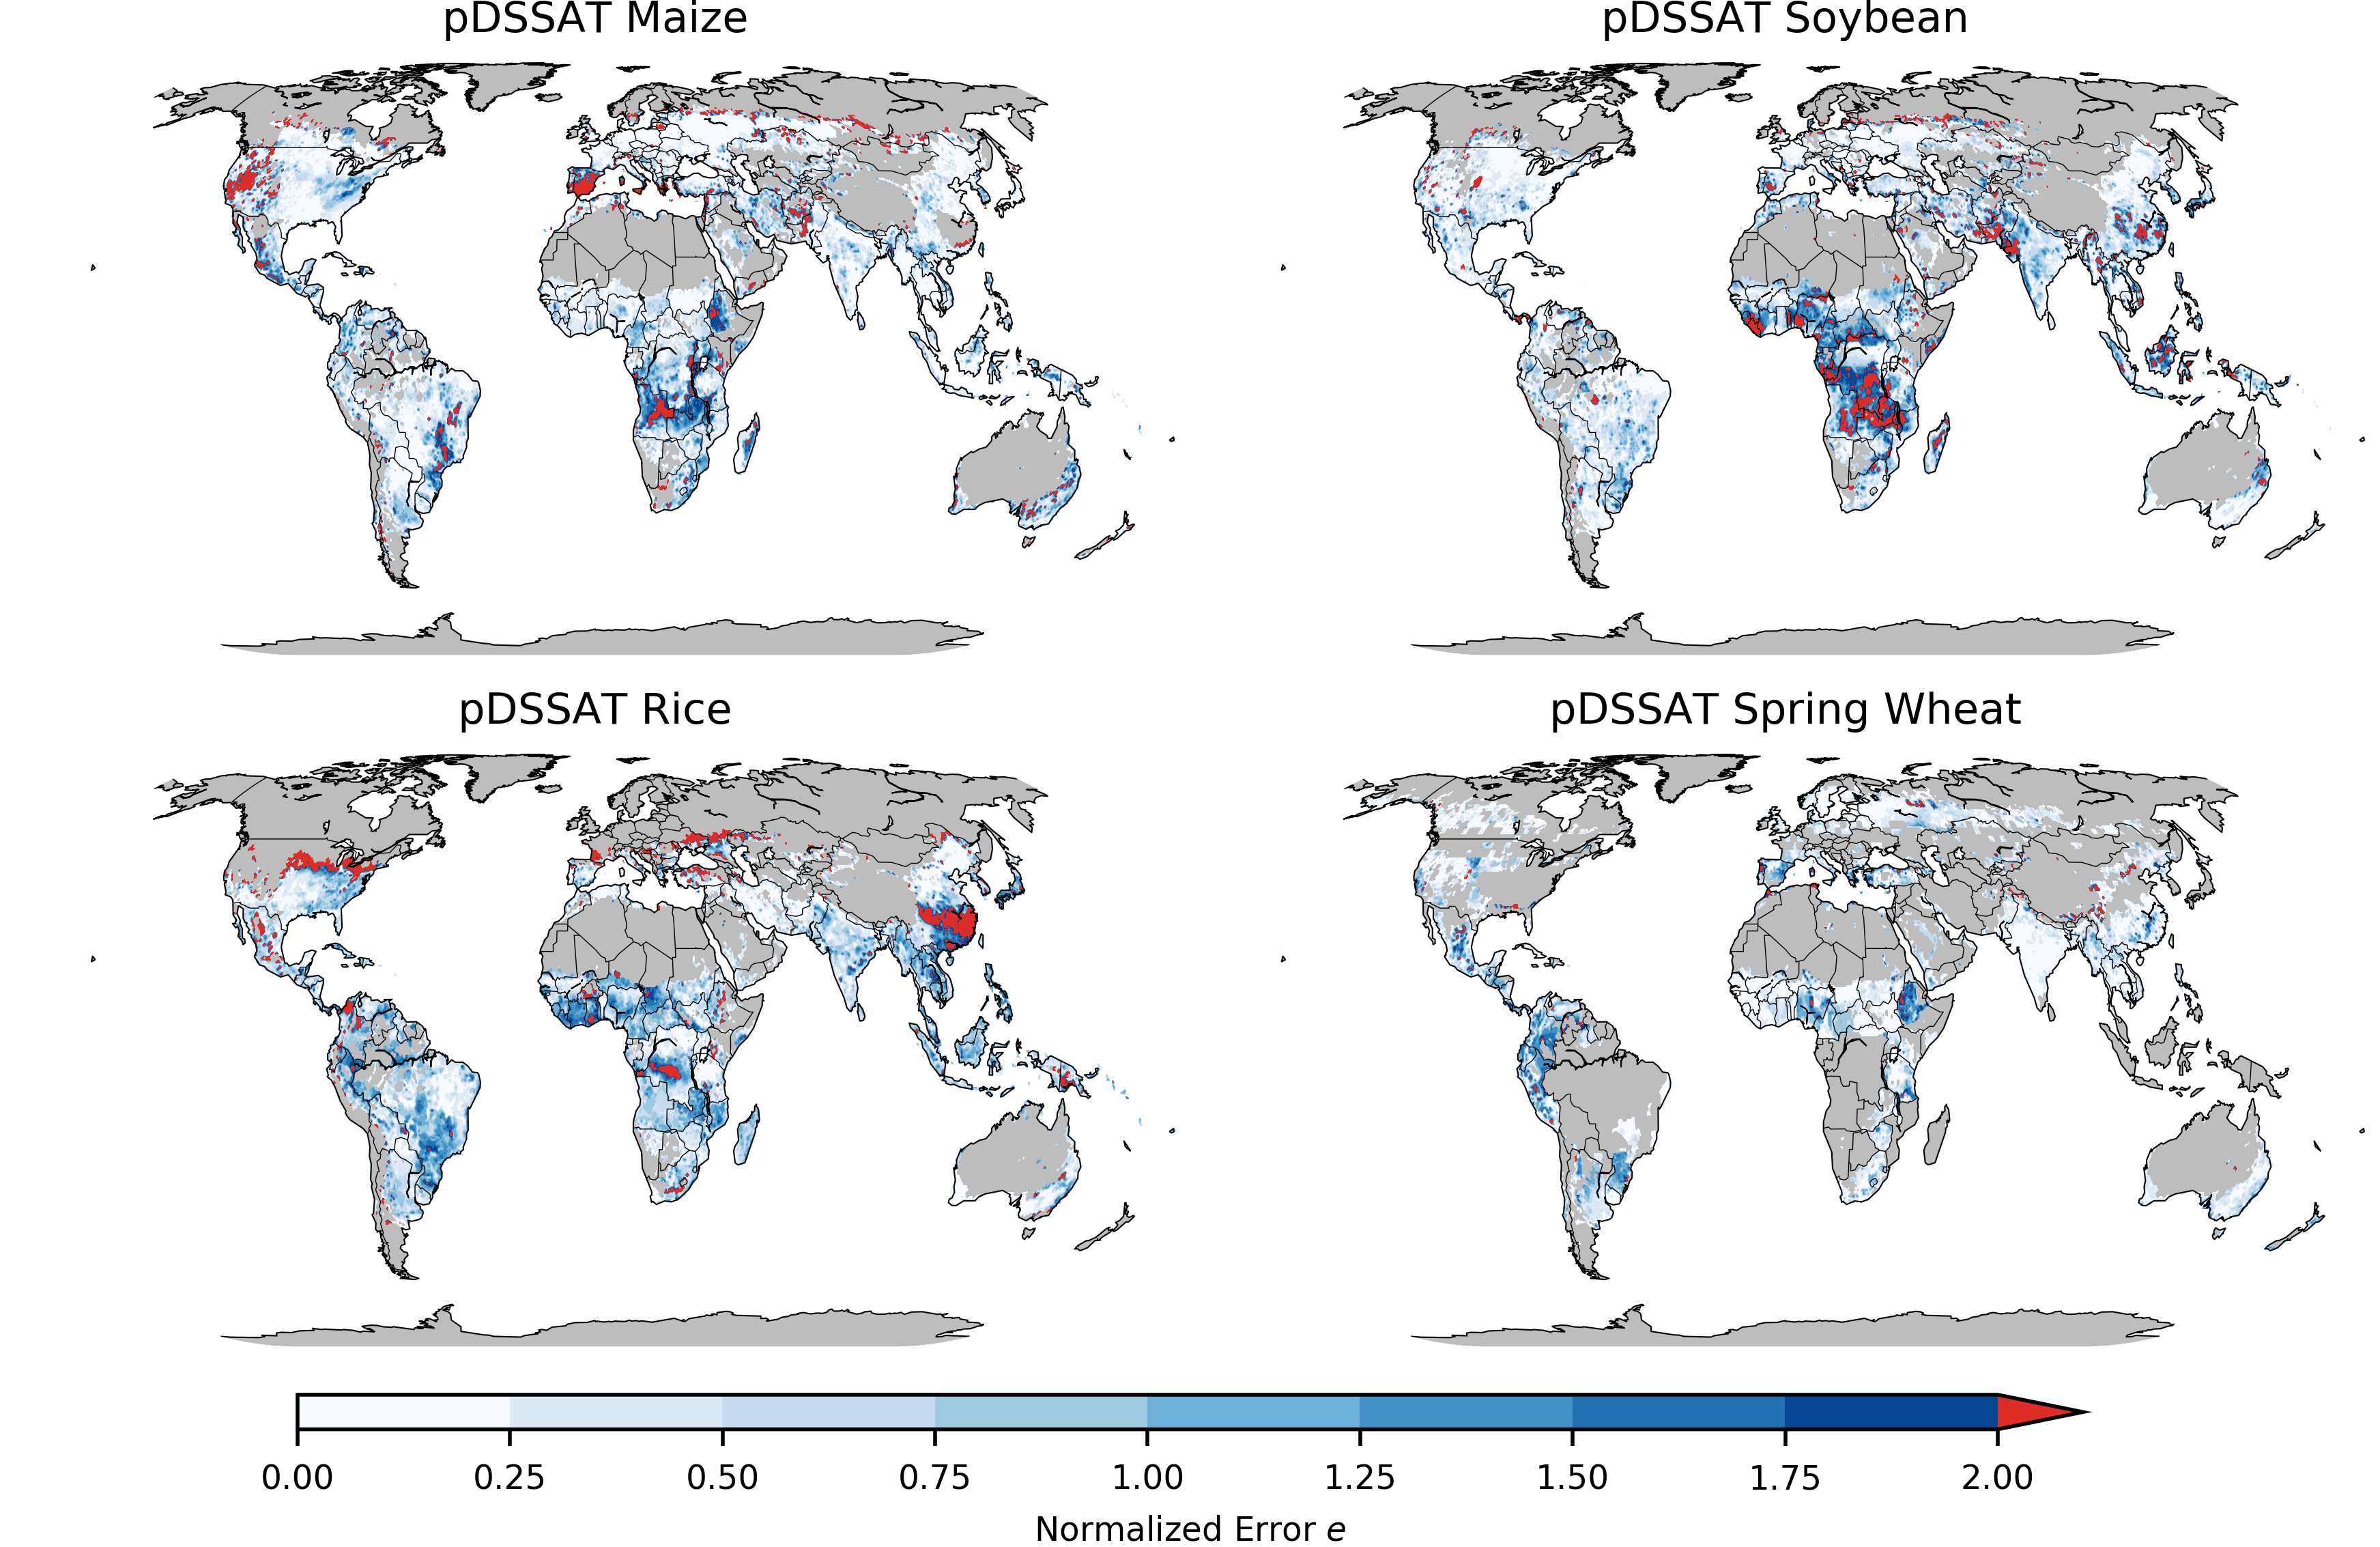
\includegraphics[width=15.5cm]{pDSSAT_spatial_error.png}
  \caption{Normalized error $e$ for pDSSAT. Same convention as main text Figure 8.}
\end{figure}

\begin{figure}[h!]
  \centering
  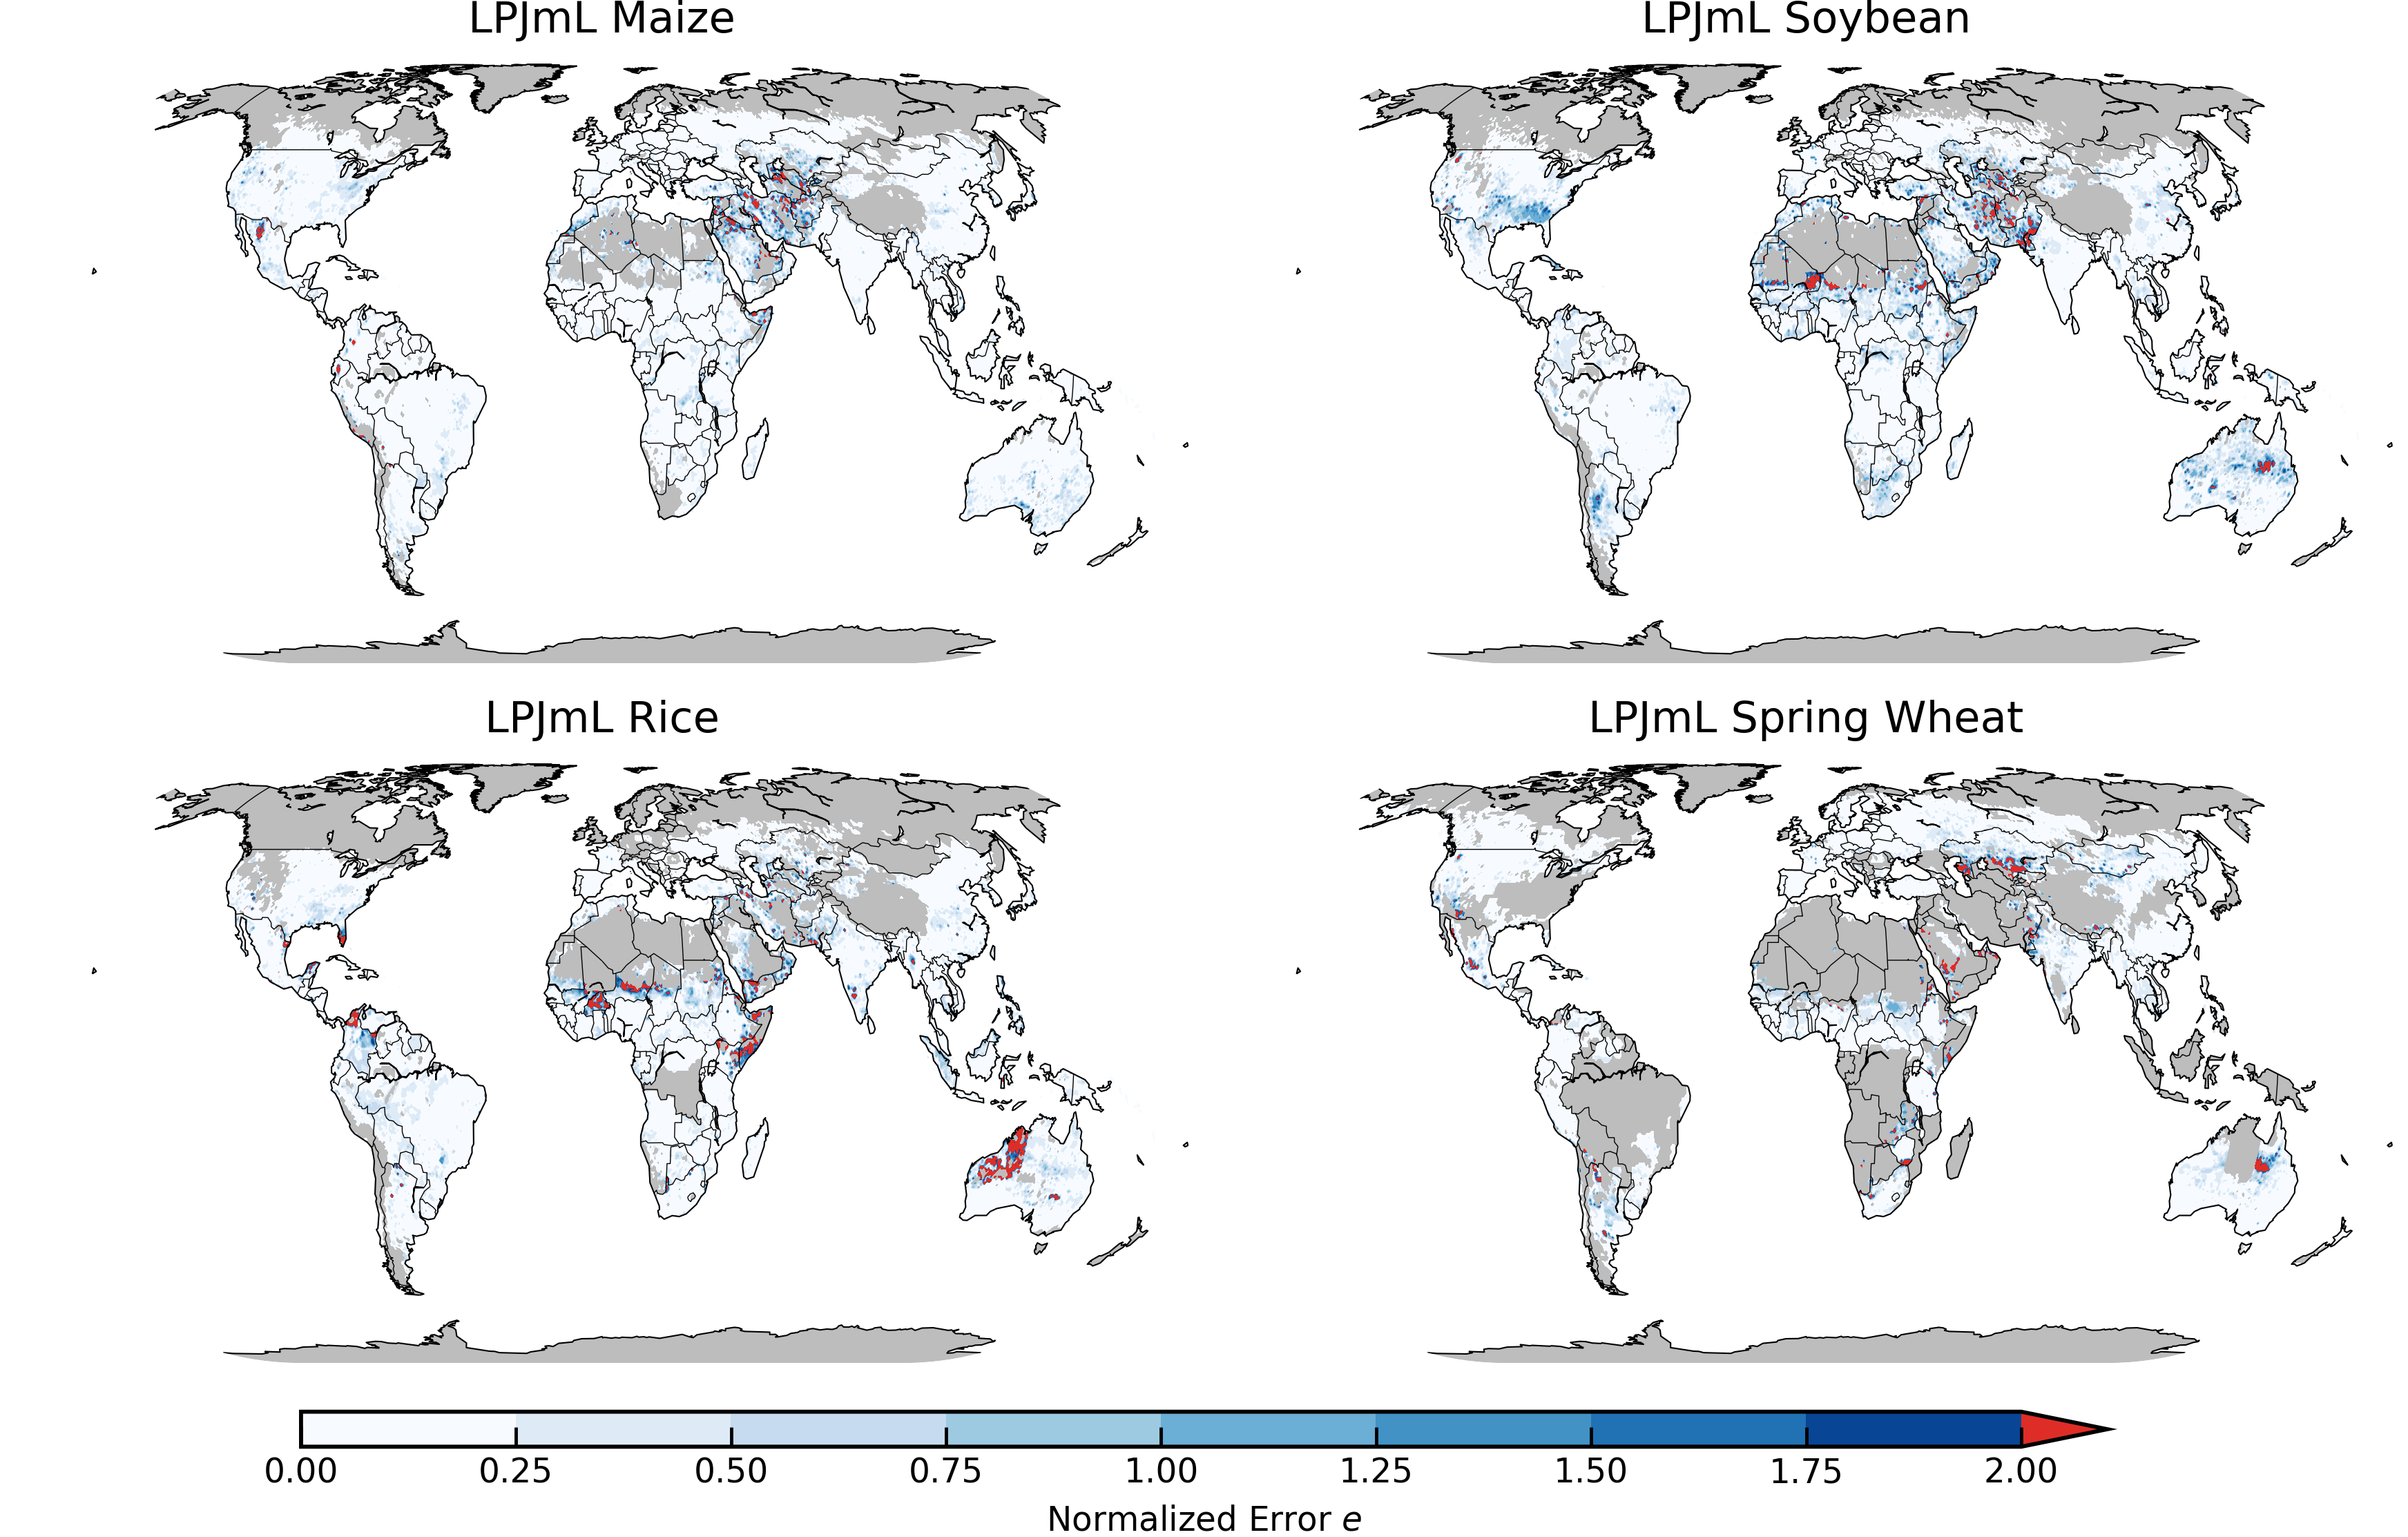
\includegraphics[width=15.5cm]{LPJmL_spatial_error.png}
  \caption{Normalized error $e$ for LPJmL. Same convention as main text Figure 8.}
\end{figure}

\begin{figure}[h!]
  \centering
  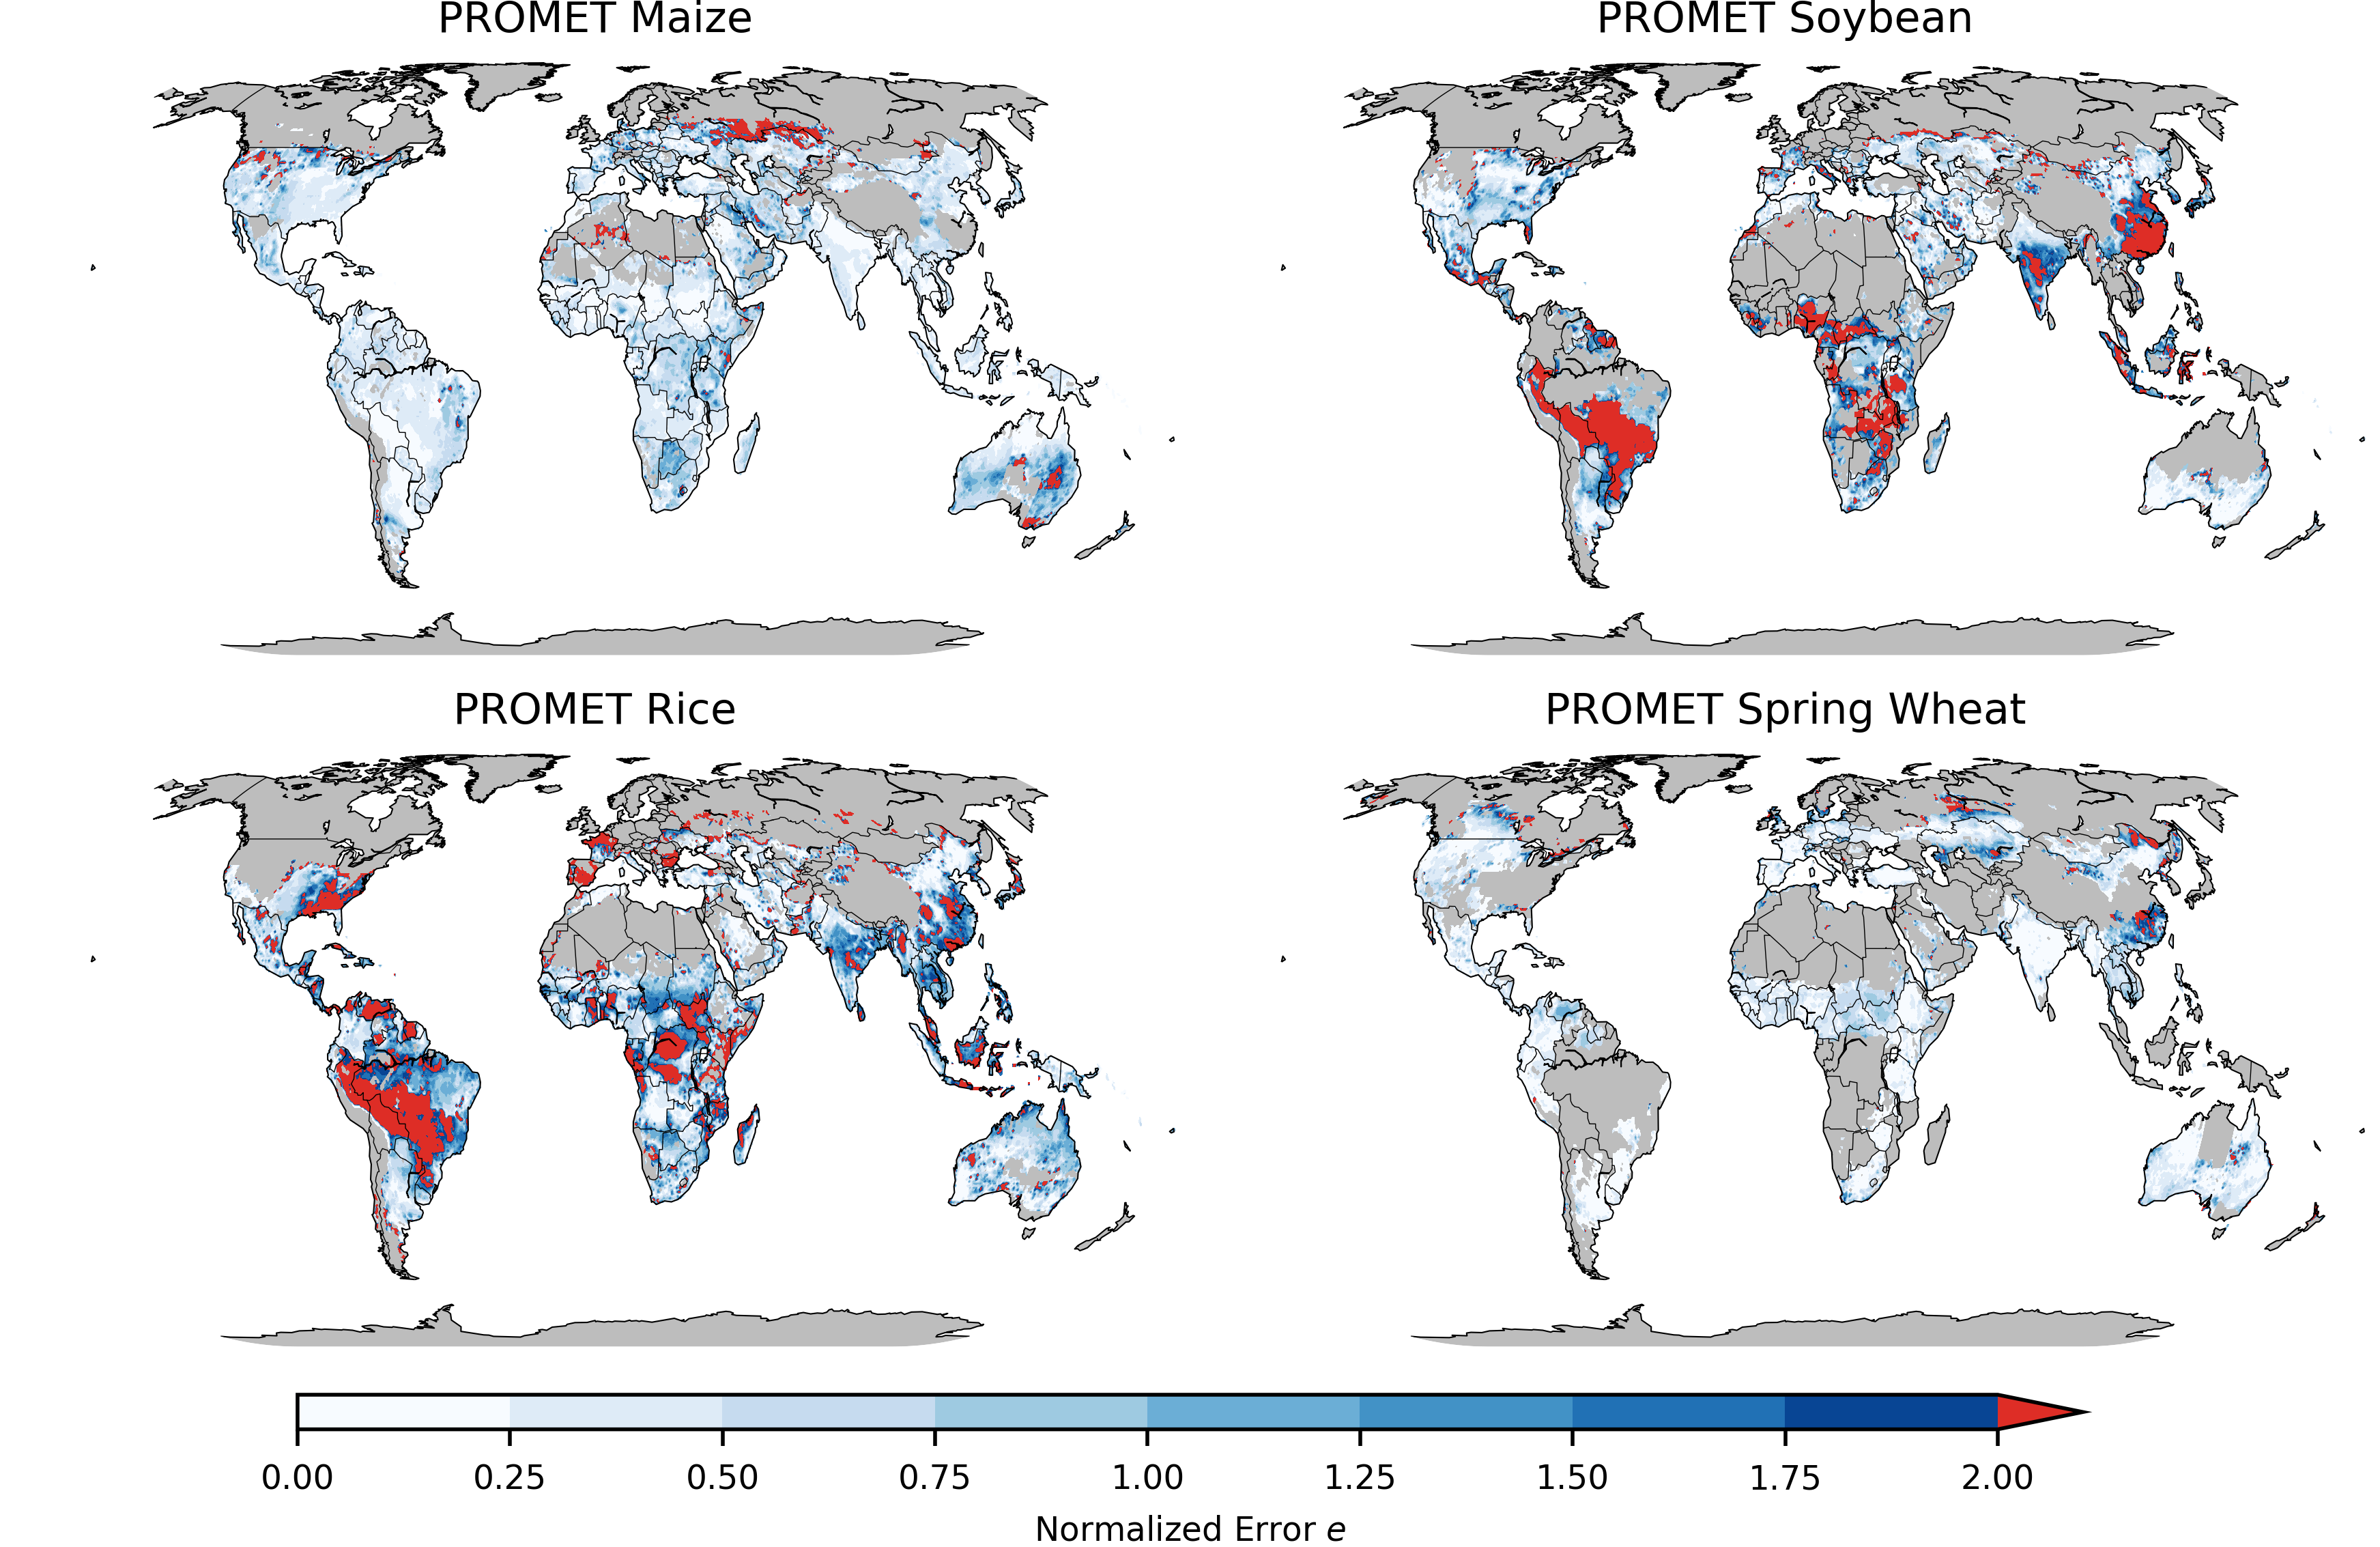
\includegraphics[width=15.5cm]{PROMET_spatial_error.png}
  \caption{Normalized error $e$ for PROMET. Same convention as main text Figure 8.}
\end{figure}

\begin{figure}[h!]
  \centering
  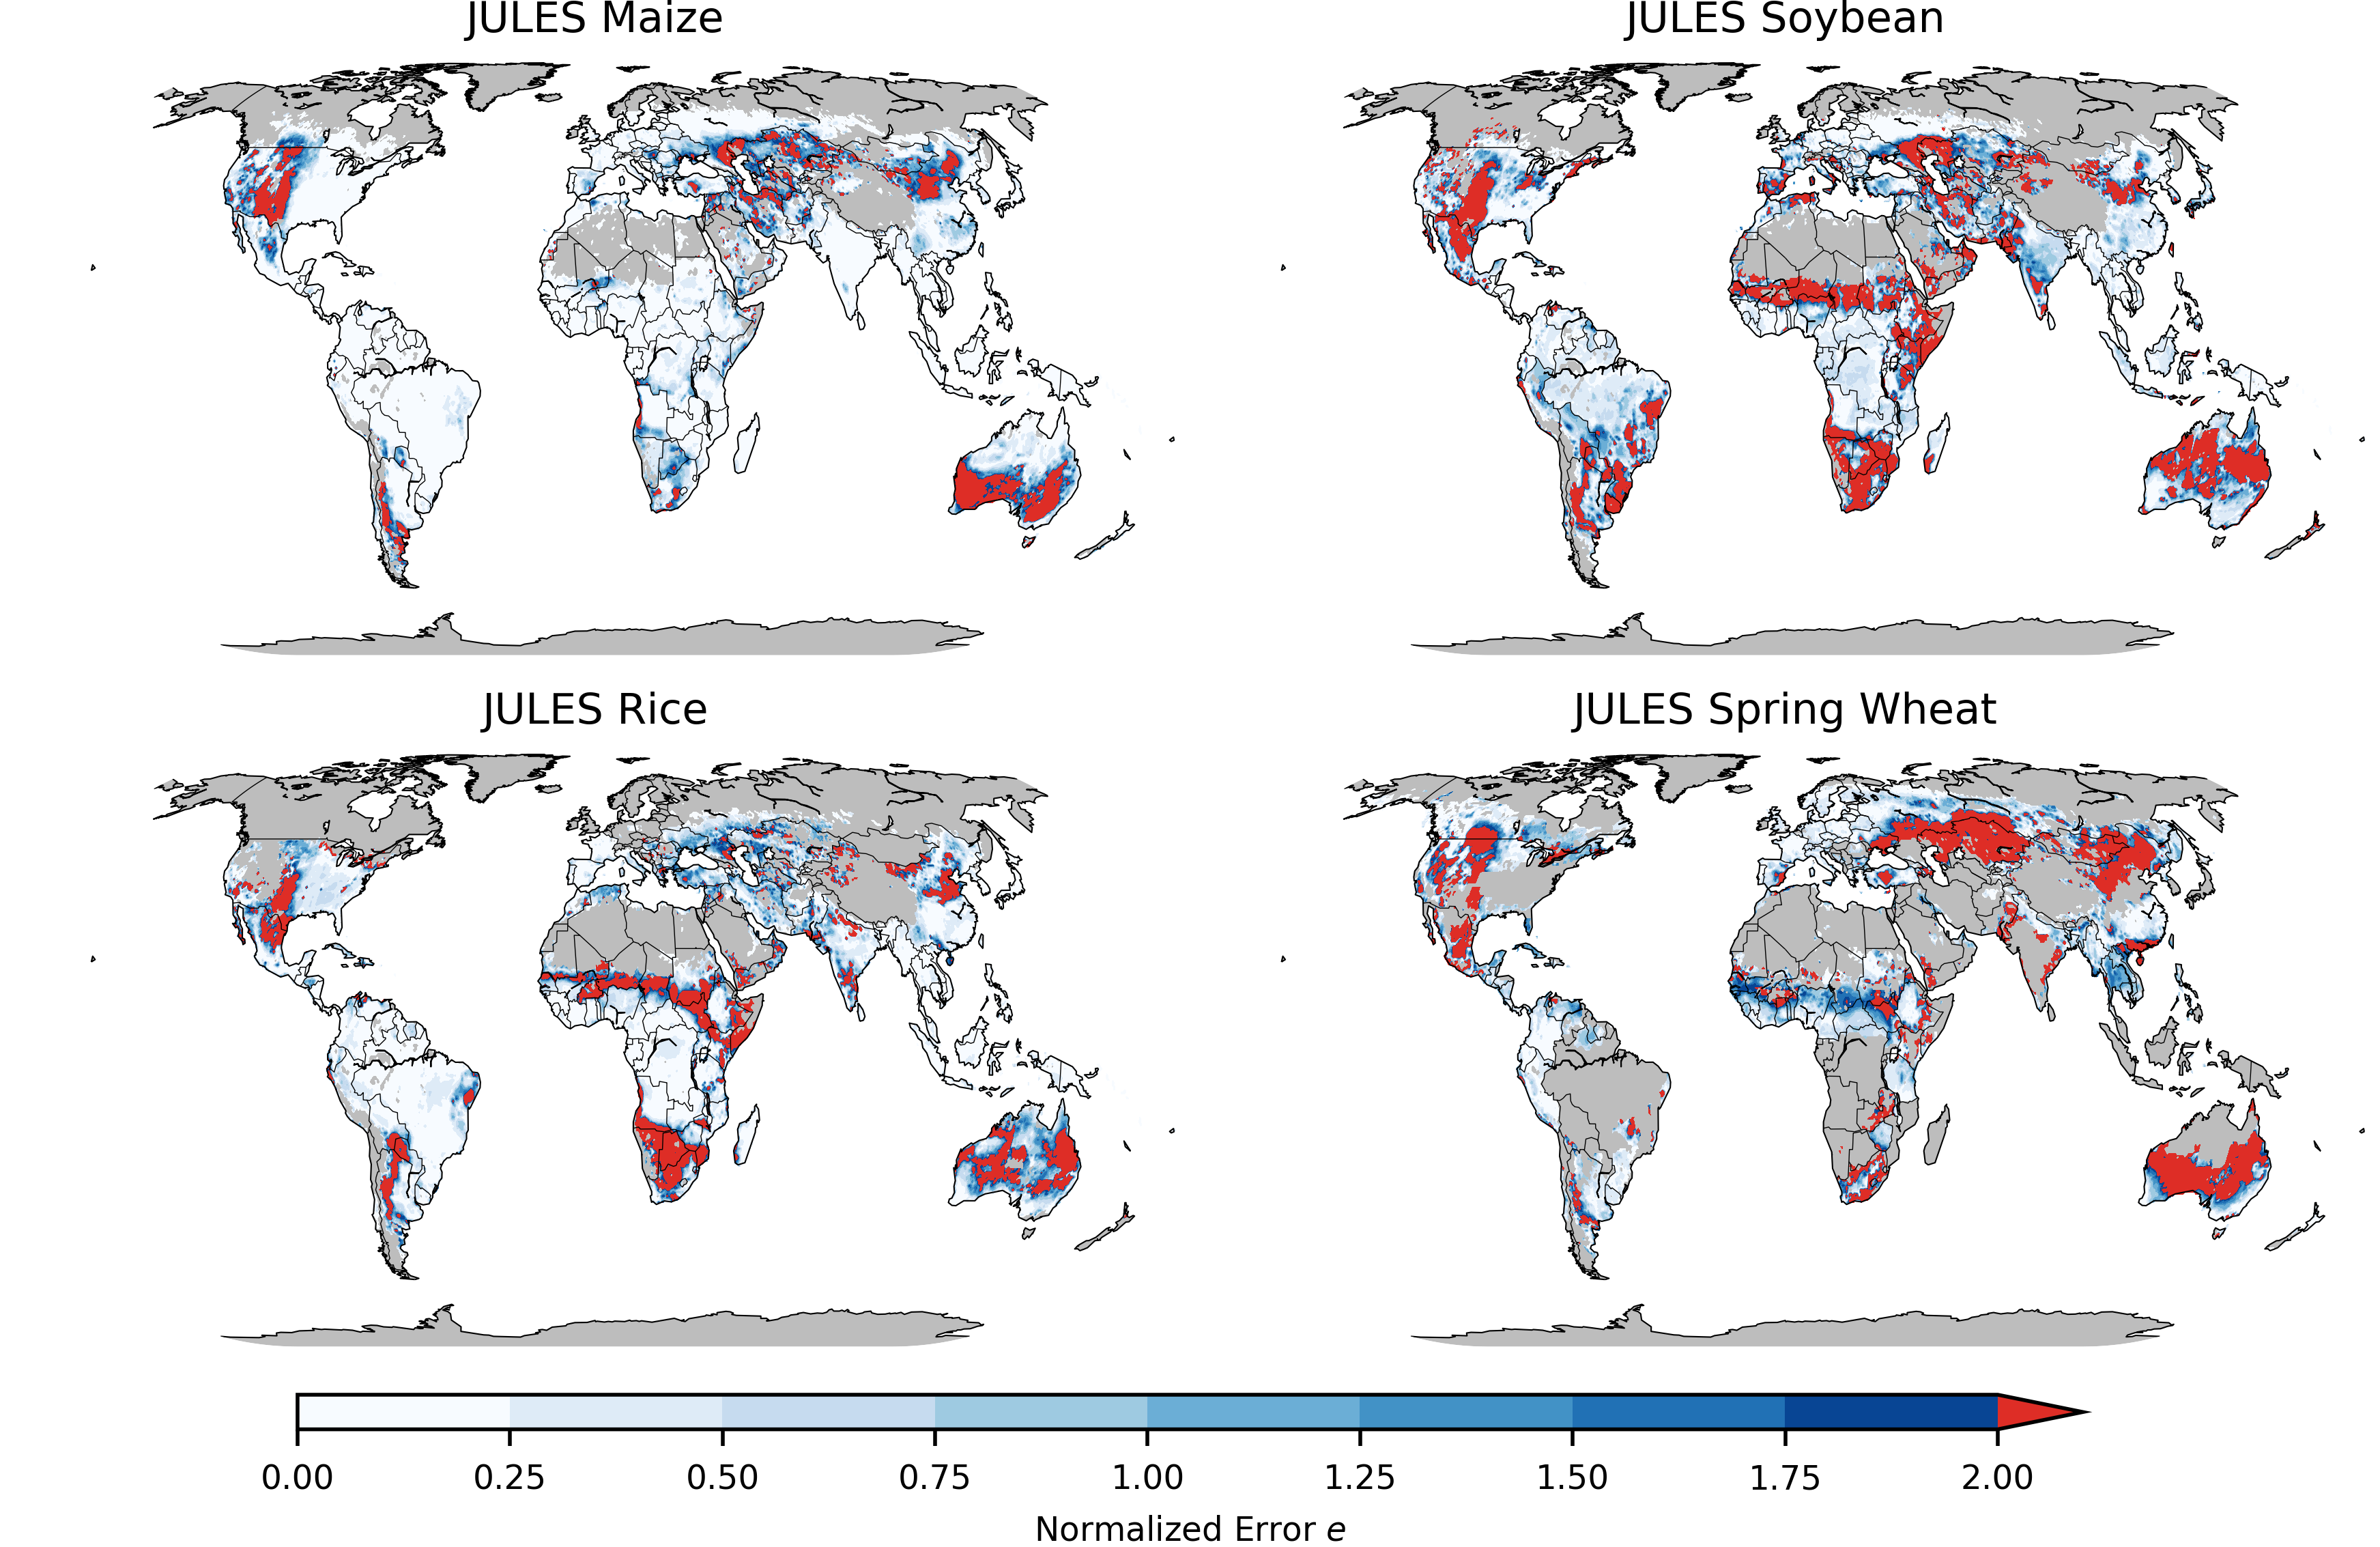
\includegraphics[width=15.5cm]{JULES_spatial_error.png}
  \caption{Normalized error $e$ for JULES. Same convention as main text Figure 8.}
\end{figure}

\begin{figure}[h!]
  \centering
  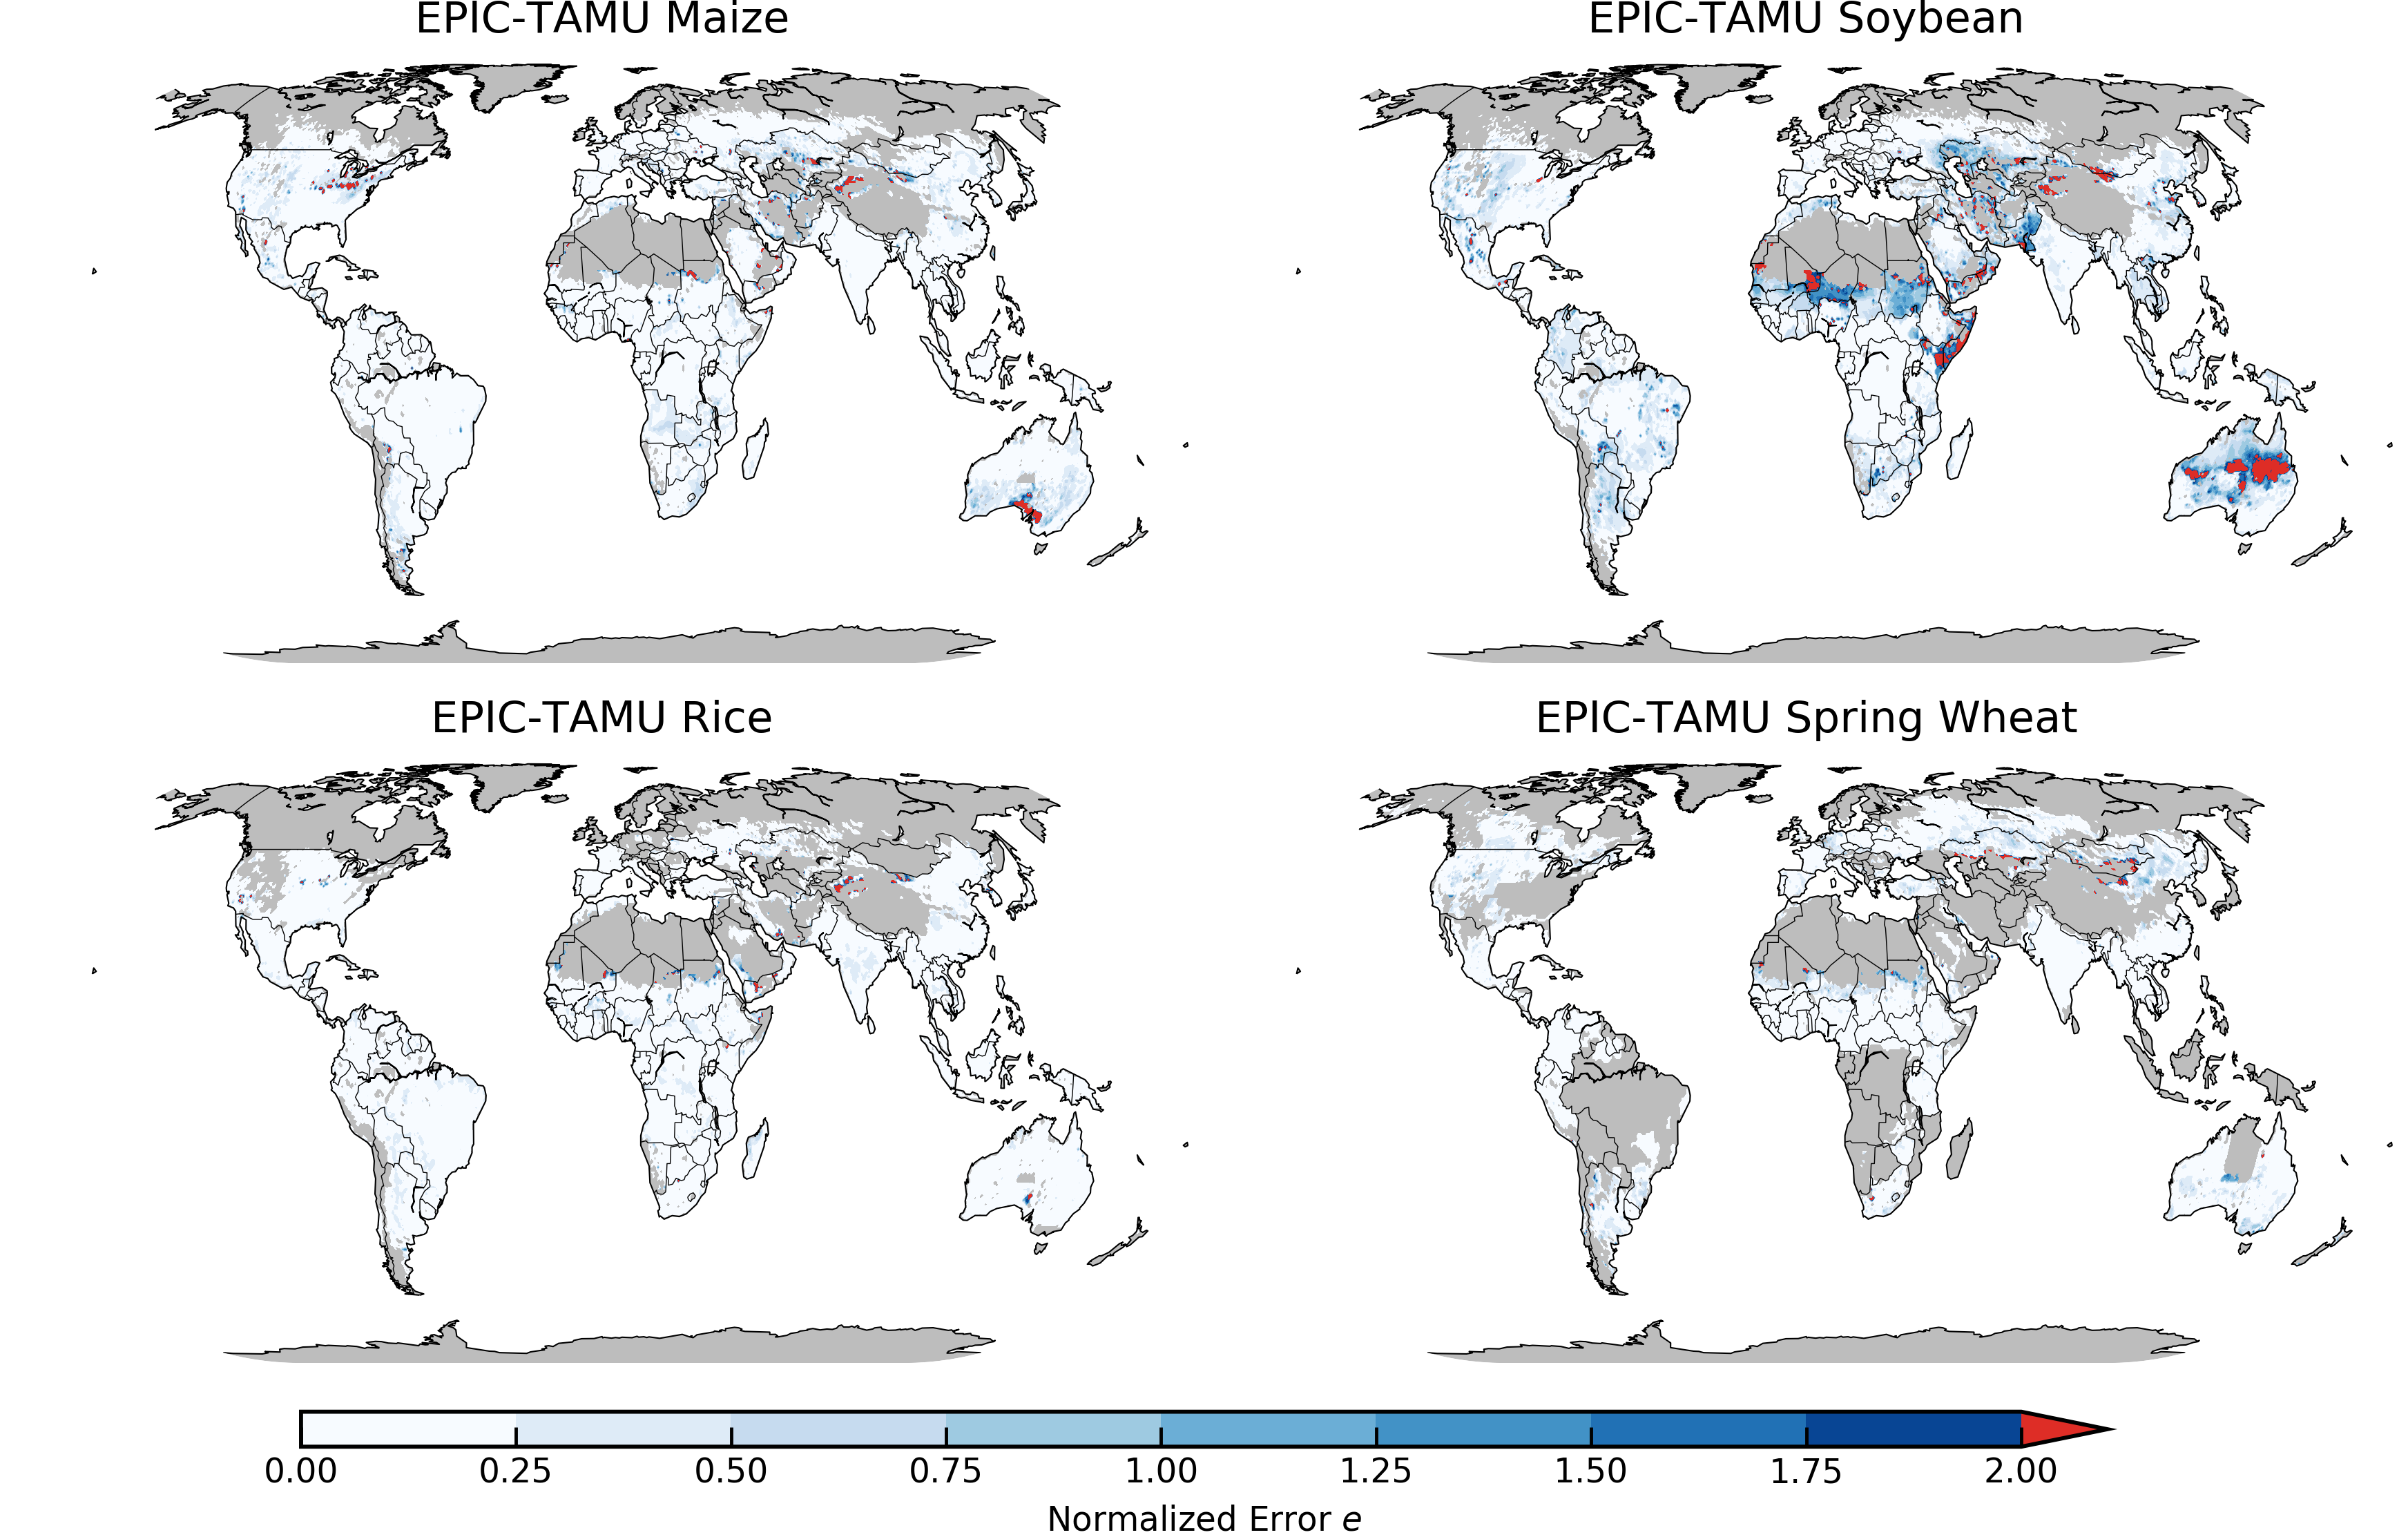
\includegraphics[width=15.5cm]{EPIC-TAMU_spatial_error.png}
  \caption{Normalized error $e$ for EPIC-TAMU. Same convention as main text Figure 8.}
\end{figure}

\begin{figure}[h!]
  \centering
  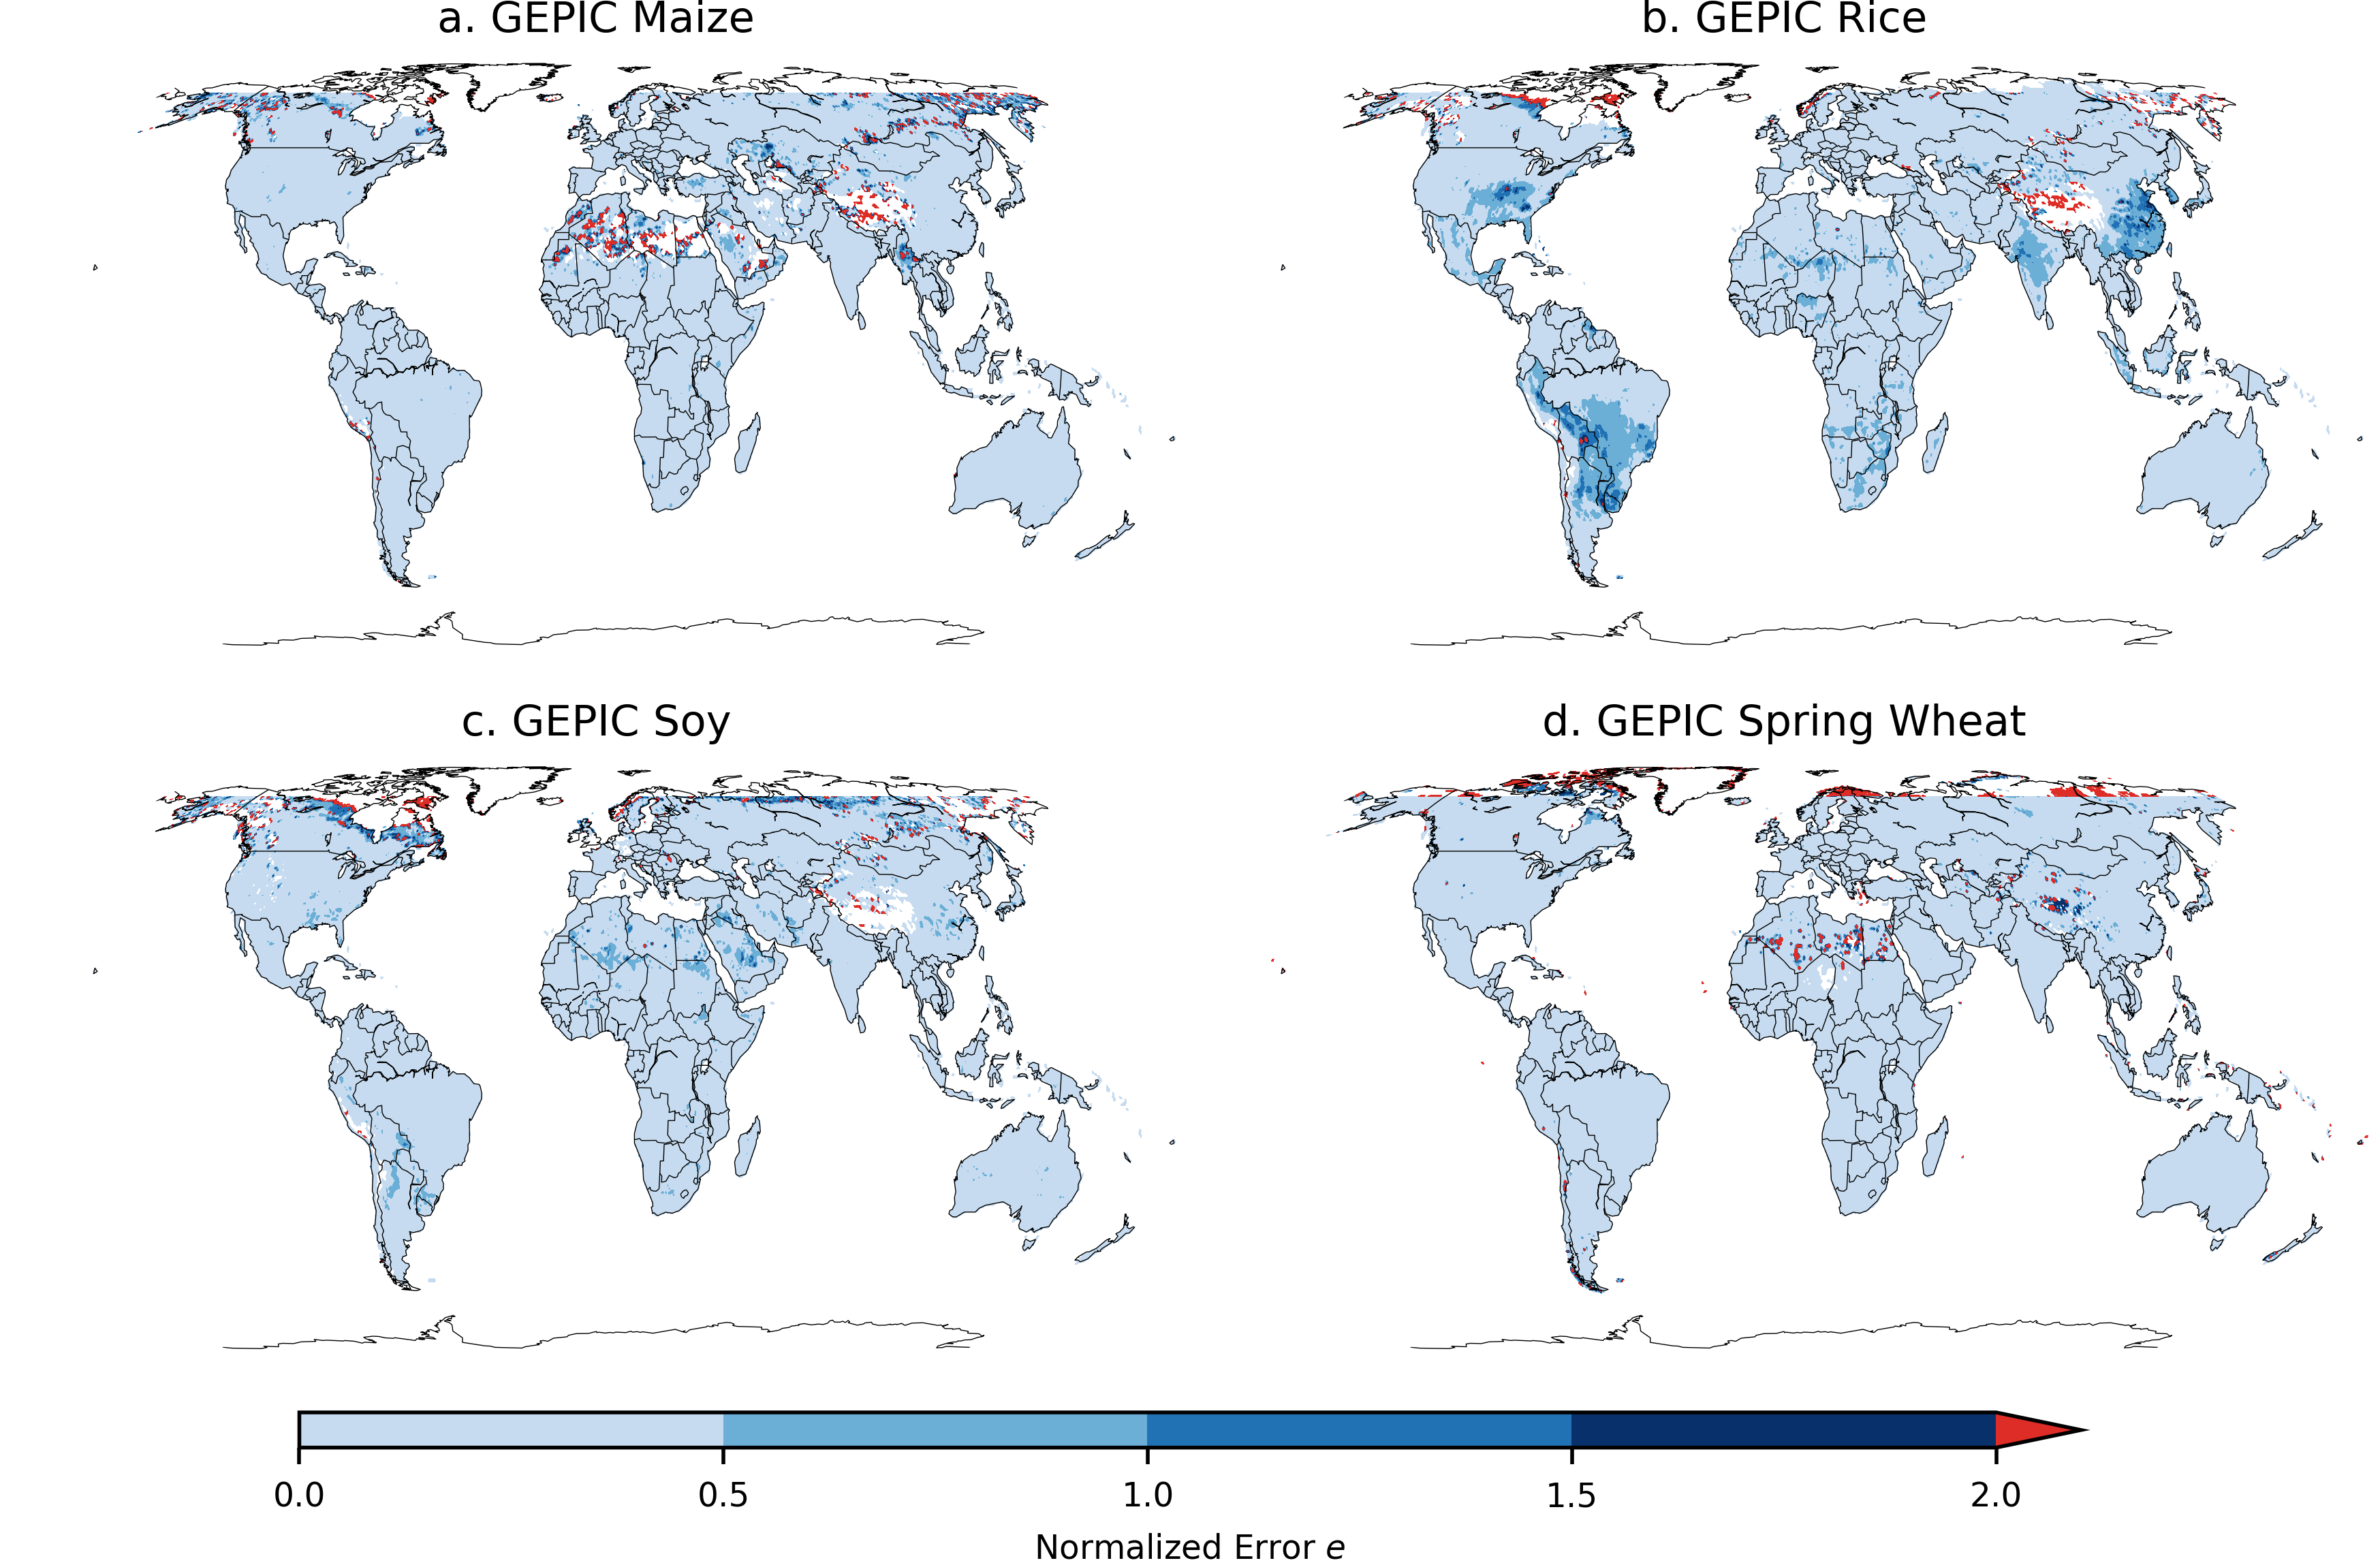
\includegraphics[width=15.5cm]{GEPIC_spatial_error.png}
  \caption{Normalized error $e$ for GEPIC. Same convention as main text Figure 8.}
\end{figure}

\begin{figure}[h!]
  \centering
  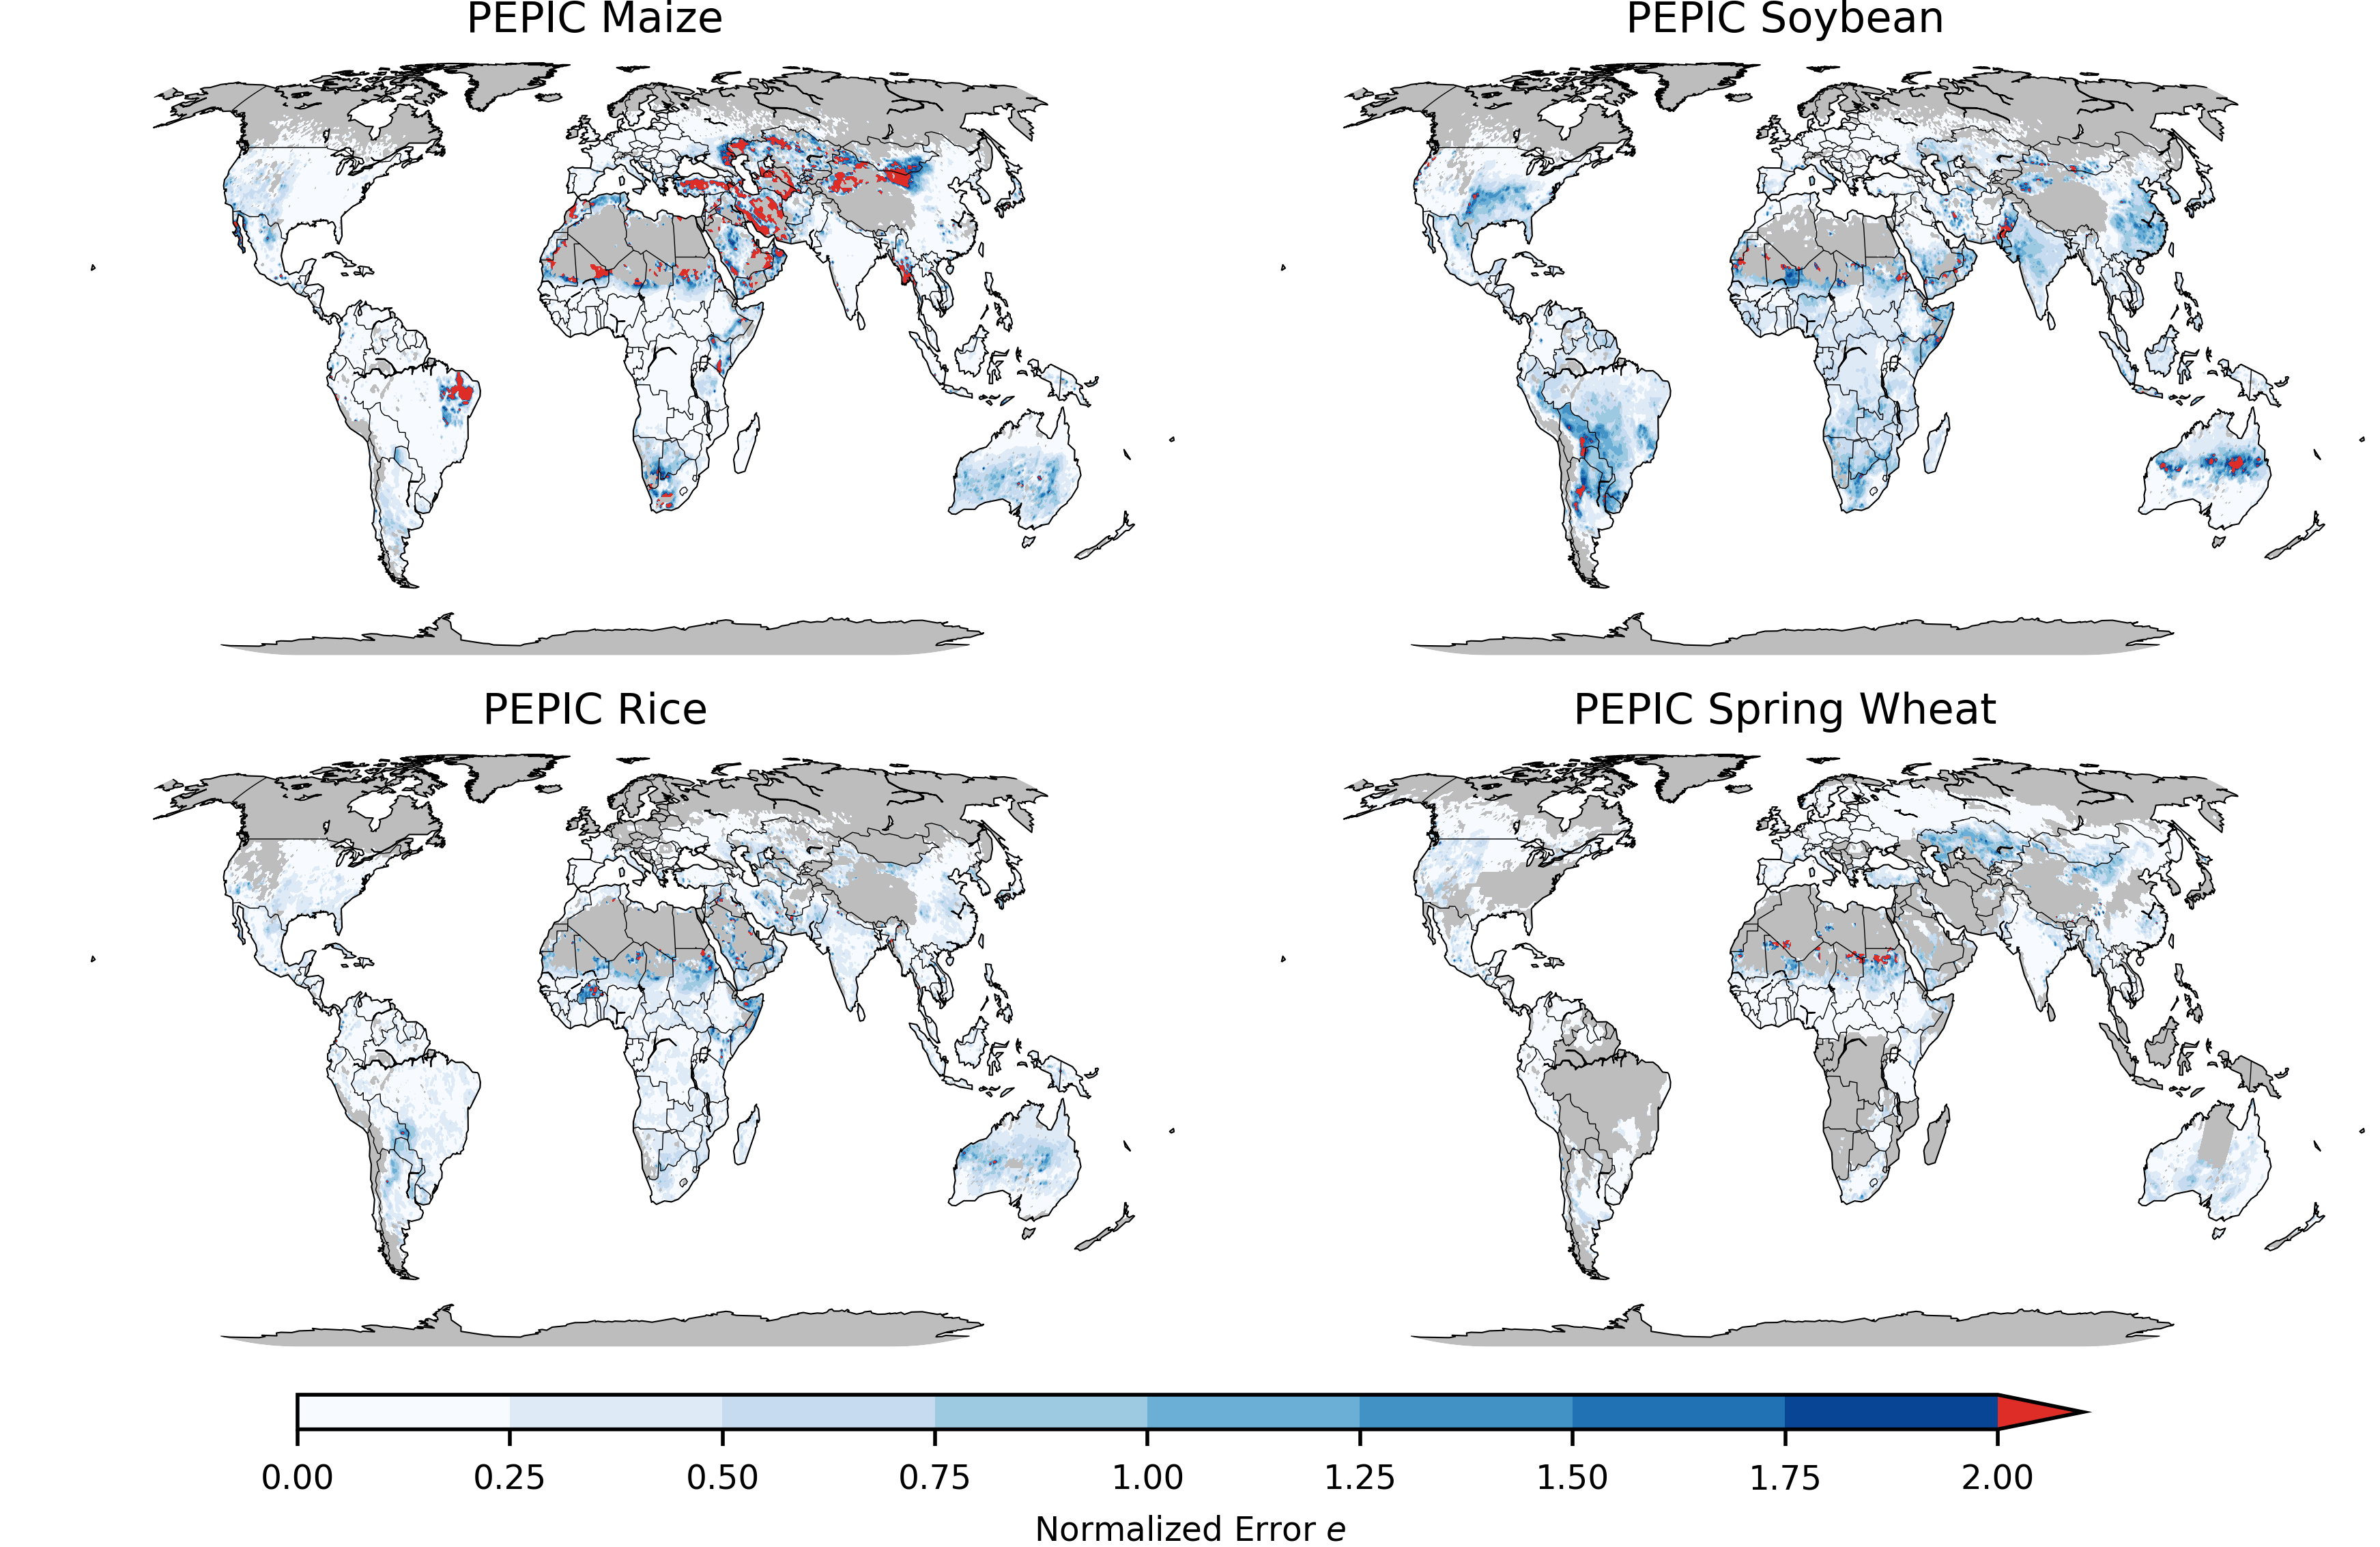
\includegraphics[width=15.5cm]{PEPIC_spatial_error.png}
  \caption{Normalized error $e$ for PEPIC. Same convention as main text Figure 8.}
\end{figure}

%%%%%%%%%%%%%%%%%%%%%%%%%%%%%%%%%%%%%%%%%%%%%%%%%%%%%%%%%%%%%%%%%%%%%%%%%%%%%%%%%%%%%%%%%%%%%%%%%%%%%%%%%%%%%%%%
%%%%%%%%%%%%%%%%%%%%%%%%%%%%%%%%%%%%%%%%%%%%%%%%%%%%%%%%%%%%%%%%%%%%%%%%%%%%%%%%%%%%%%%%%%%%%%%%%%%%%%%%%%%%%%%%
%%%%%%%%%%%%%%%%%%%%%%%%%%%%%%%%%%%%%%%%%%%%%%%%%%%%%%%%%%%%%%%%%%%%%%%%%%%%%%%%%%%%%%%%%%%%%%%%%%%%%%%%%%%%%%%%
%%%%%%%%%%%%%%%%%%%%%%%%%%%%%%%%%%%%%%%%%%%%%%%%%%%%%%%%%%%%%%%%%%%%%%%%%%%%%%%%%%%%%%%%%%%%%%%%%%%%%%%%%%%%%%%%
